\documentclass[12pt, a4paper]{report} % extreport
\usepackage[margin=1.75cm]{geometry}
\usepackage{amsmath, mathtools}
\usepackage{graphicx}
\usepackage{caption}
\usepackage{subcaption}
\usepackage{float}
\usepackage{wasysym}
\usepackage[procnames]{listings}
\usepackage{color}
\usepackage{multirow}
\setlength\parindent{24pt}

\usepackage{fancyhdr}
\pagestyle{fancy}
\fancyhf{}
\rhead{Nonlinear Dynamics - Take home exam}
\lhead{Koorosh Gobal}
\rfoot{Page \thepage}
\lfoot{\today}

\definecolor{keywords}{RGB}{255,0,90}
\definecolor{comments}{RGB}{0,0,113}
\definecolor{red}{RGB}{160,0,0}
\definecolor{green}{RGB}{0,150,0}
 
\lstset{language=Python, 
        basicstyle=\ttfamily\small, 
        keywordstyle=\color{keywords},
        commentstyle=\color{comments},
        stringstyle=\color{red},
        showstringspaces=false,
        identifierstyle=\color{green},
        procnamekeys={def,class}}
% ===============================================================
\begin{document}
%\begin{tabularx}{\textwidth}{Xr Xl}
%\textbf{Koorosh Gobal} & \textbf{Nonlinear Dynamics - Take Home Exam}
%\end{tabularx}
\textbf{Problem definition}:
A physical problem has the governing equation
%
\begin{equation}\label{eq:governingEquation}
	\left(
	1 + \frac{\epsilon u^2}{1 - u^2}
	\right) \ddot{u} +
	\frac{\epsilon u \dot{u}^2}{\left( 1 - u^2 \right)^2} +
	\frac{k}{m_1}u +
	\frac{\epsilon g u}{l \sqrt{1 - u^2}} = 
	0
\end{equation}
%
Apply Taylor series expnasions to eliminate the denominators while retaining all terms up to cubic terms. Identify the stationary (points) and define its (their) characteristics.

\noindent\hrulefill

% -------------------------------------------------------------------
\textbf{Solution approach:}
Equation \eqref{eq:governingEquation} governs a physical problem, therefore, the solution needs to always be in the real domain. Therefore, the value under the square root in Equation \eqref{eq:governingEquation} needs to be always positive for a real solution.

\begin{equation}\label{eq:solutionBound}
	1 - u^2 > 0 \Longrightarrow -1 < u < 1
\end{equation}

A \emph{stationary point} or \emph{critical point} of a differentiable function of one variable is a point of the domain of the function where the derivative is zero. To find the stationary point of Equation \eqref{eq:governingEquation}, we set $\dot{u}$ equal to zero. This also means that $\ddot{u}$ is zero as well.

\begin{align*}
	\dot{u} = \ddot{u} = 0 &\rightarrow
	\frac{k}{m_1}u + \frac{\epsilon g u}{l \sqrt{1 - u^2}} = 0 \\
	&\rightarrow
	u \left[
		\frac{k}{m_1} + \frac{\epsilon g}{l \sqrt{1 - u^2}}
	  \right] = 0
\end{align*}

Therefore,

\begin{subequations}
\begin{align}
	u = 0 \\
	\frac{k}{m_1} + \frac{\epsilon g}{l \sqrt{1 - u^2}} = 0 \label{eq:fixedPoint2}
\end{align}
\end{subequations}

First fixed point is the origin, ($u = 0$). To find the second fixed point we need to solve Equation \eqref{eq:fixedPoint2} for $u$.

\begin{equation}\label{eq:fixedPointDerivation}
\begin{aligned}
	\frac{k}{m_1} + \frac{\epsilon g}{l \sqrt{1 - u^2}} &= 0 \rightarrow \\
	\frac{1}{\sqrt{1 - u^2}} &= -\frac{kl}{m_1 \epsilon g} \rightarrow \\
	u &= \pm \sqrt{1 - \left( \dfrac{m_1 \epsilon g}{kl} \right)^2}
\end{aligned}
\end{equation}

To calculate these two fixed points we need to choose our system's constants, i.e. $m_1$, $\epsilon$, $g$, $k$, and $l$. However, for the second and third stationary points exists, system constants need to satisfy the following conditions. As can be seen in the second line of Equation \eqref{eq:fixedPointDerivation}, $\dfrac{m_1 \epsilon g}{kl}$ needs to be negative. Moreover, it should be between \lq\lq$-1$\rq\rq\ and \lq\lq$1$\rq\rq\ so that the value of stationary point is real. This can be seen in the third line of Equation  \eqref{eq:fixedPointDerivation}. These two conditions can be written as

\begin{equation}\label{eq:stationaryPointCondition}
	-1 < \dfrac{m_1 \epsilon g}{kl} < 0
\end{equation}

In order to define the characteristics of the stationary points, the first step is to linearise the governing equations near the stationary point. To achieve this, the governing equation is written in the state space form.

We define the following variables

\begin{align*}
	x_1 &= u \\
	x_2 &= \dot{x}_1 = \dot{u}
\end{align*}

Equation \eqref{eq:governingEquation} can be written in terms of these new variables.

\begin{equation}\label{eq:stateEquation}
\begin{aligned}
	\dot{x}_1 &= x_2 \\
	\dot{x}_2 &=
	-\left[
	\frac{\epsilon x_1 x_2^2}{\left( 1 - x_1^2 \right)^2} +
	\frac{k}{m_1} x_1 +
	\frac{\epsilon g x_1}{l \sqrt{1 - x_1^2}}
	\right] \bigg/
	\left(
	1 + \frac{\epsilon x_1^2}{1 - x_1^2}
	\right)
\end{aligned}
\end{equation}

The \emph{Taylor series expansion} for a multi-variable function $f(x, y)$ at $(a, b)$ is defined as

\begin{equation}\label{eq:taylorSeriesExpansion}
\begin{aligned}
	f(x,y) = &f(a,b) + \\
		&f_x(a,b)(x-a) + f_y(a,b)(y-b) + \\
		&\frac{1}{2} \left[
 	 				 f_{xx}(a,b)(x-a)^2 + 
 					 2f_{xy}(a,b)(x-a)(y-b) +
 					 f_{yy}(a,b)(y-b)^2
		             \right] \\
		&\begin{split} \frac{1}{3!}
					  \left[
					  f_{xxx}(a,b)(x-a)^3 +
					  3f_{xxy}(a,b)(x-a)^2(y-b) +
					  \right.\\
					  \left.
					  3f_{xyy}(a,b)(x-a)(y-b)^2 +
					  f_{yyy}(a,b)(y-b)^3
					  \right]
					  \end{split}		              
\end{aligned}
\end{equation}

We use Equation \eqref{eq:taylorSeriesExpansion} to linearise Equation \eqref{eq:stateEquation}. This is done by assuming the right-hand-side of the state equation is a function of $x_1$ and $x_2$. We used \texttt{sympy} library in \texttt{Python} to calculate the derivatives of Equation \eqref{eq:stateEquation}. The code is available in the appendix. The linearised function around $(0, 0)$ can be written as

\begin{equation}\label{eq:StateEquationAt0}
\begin{aligned}
	\dot{y}_1 &= y_2 \\
	\dot{y}_2 &= y_{1} \left(- \frac{\epsilon}{l} g - \frac{k}{m_{1}}\right) - 
	\epsilon y_{1} y_{2}^{2} + 
	\frac{1}{6} y_{1}^{3} \left[- \frac{3 \epsilon}{l} g + 6 \epsilon \left(\frac{\epsilon}{l} g + \frac{k}
	{m_{1}}\right)\right]
\end{aligned}
\end{equation}

The state equation \eqref{eq:stateEquation} can also be linearized around other stationary points (Equation \eqref{eq:fixedPointDerivation}). However, we end up with very long symbolic equations that can not be easily displayed.

To plot the phase portrait and trajectories, we revisit Equation \eqref{eq:stateEquation}. Equation \eqref{eq:solutionBound} defined the bounds on $x_1$. From what we derived earlier, it is clear that the stationary point of $(0, 0)$ always exists. However, if the condition of Equation \eqref{eq:stationaryPointCondition} is satisfied, we get two extra stationary points at $(\sqrt{1 - \left( \dfrac{m_1 \epsilon g}{kl} \right)^2}, 0)$ and $(-\sqrt{1 - \left( \dfrac{m_1 \epsilon g}{kl} \right)^2}, 0)$. In what follows, we plot the phase portrait and trajectories of some random initial conditions for different values of system constants, i.e. $m_1$, $\epsilon$, $g$, $k$, and $l$. These values are shown in Table \ref{table:systemConstants}. To calculate the trajectories of the system, we use \texttt{odeint} function from \texttt{scipy.integrate} library and we integrated for $5$ seconds. This is shown in Figure \ref{fig:phasePlot}. The code is available in the appendix.

\begin{table}[htbp]
\begin{center}
\begin{tabular}{c||c|c|c|c|c|c}
case number & $\epsilon$ & $k$ & $m_1$ & $g$ & $l$ & $\dfrac{m_1 \epsilon g}{kl}$\\ \hline \hline
1 & 0.1 & 1 & 1 & 1 & 1 & 0.1 \\ \hline
2 & 0.5 & 2 & 1 & 1 & 1 & 0.25 \\ \hline
3 & 0.5 & 1 & 4 & 1 & 1 & 2 \\ \hline
4 & -0.3 & 1 & 1 & 1 & 1 & -0.3 \\ \hline
5 & -0.9 & 1 & 1 & 1 & 1 & -0.9 \\ \hline
6 & -0.5 & 1 & 3 & 1 & 1 & -1.5 \\
\end{tabular}
\end{center}
\caption{System constants}
\label{table:systemConstants}
\end{table}

\begin{figure}[H]
	\centering
	\begin{subfigure}[h]{8.0 cm}
		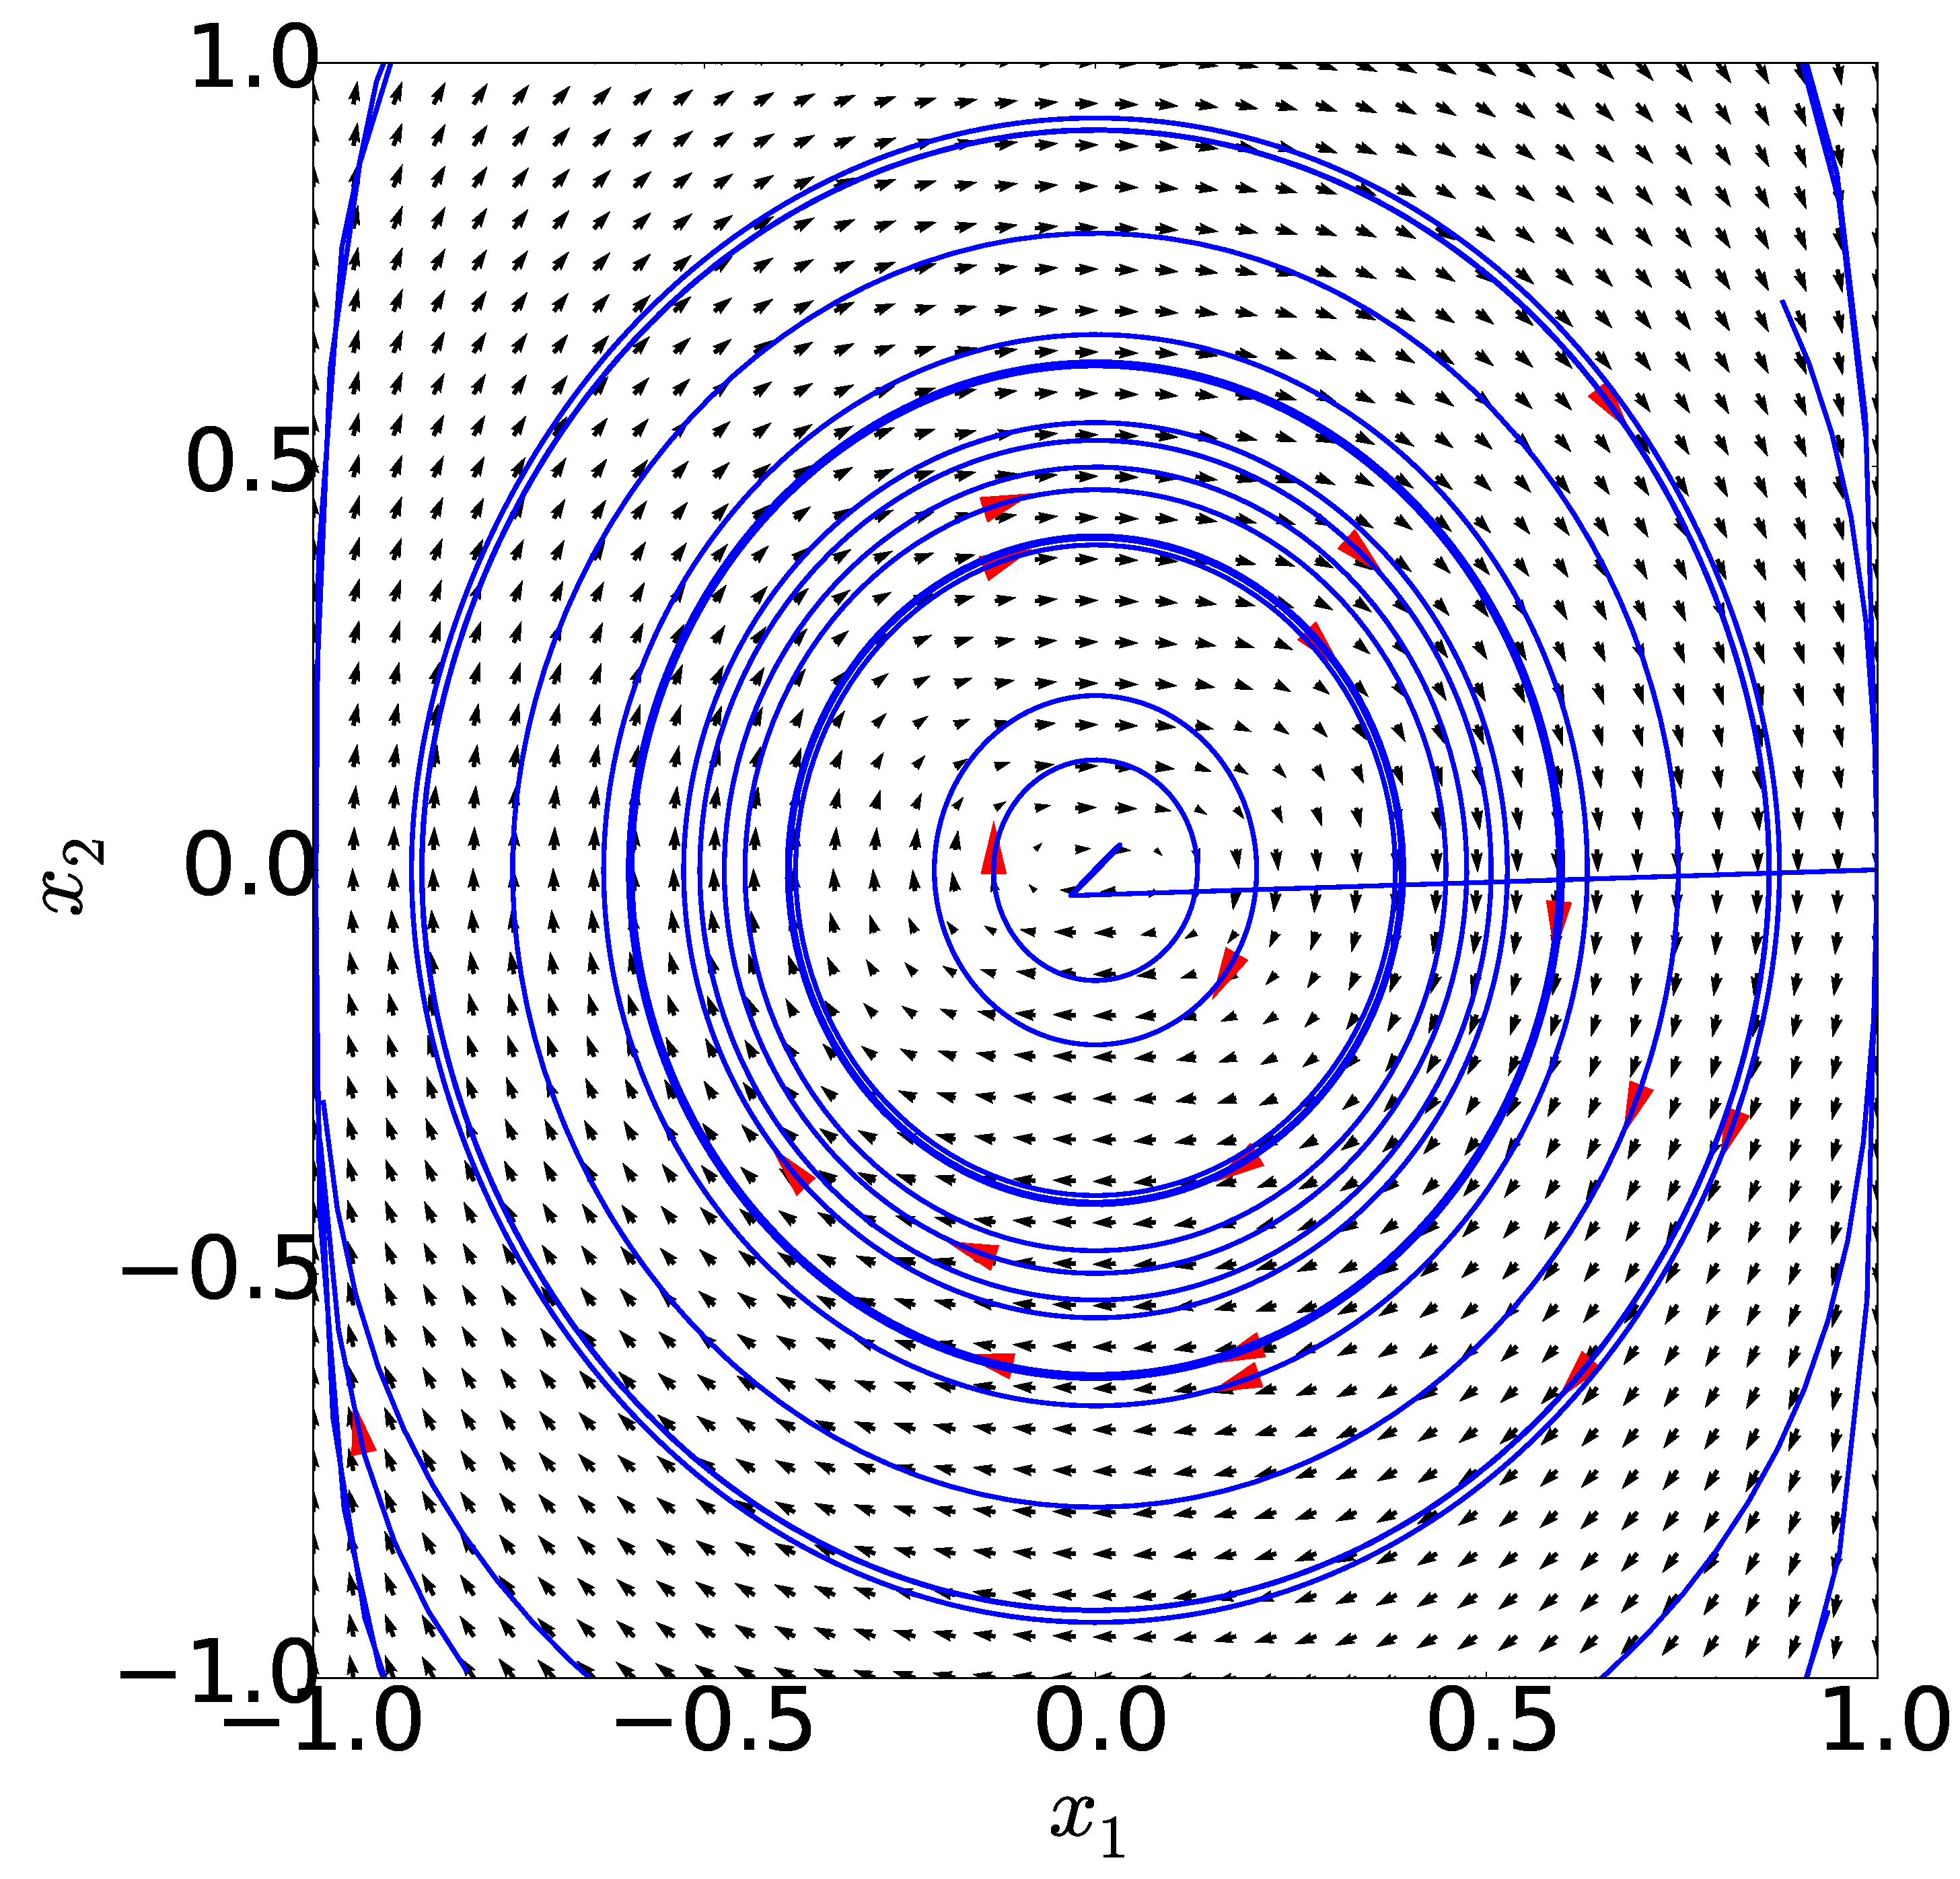
\includegraphics[width=8.0 cm]{figure/phase_portrait_1.eps}
		\caption{Case 1}
	\end{subfigure}
	\begin{subfigure}[h]{8.0 cm}
        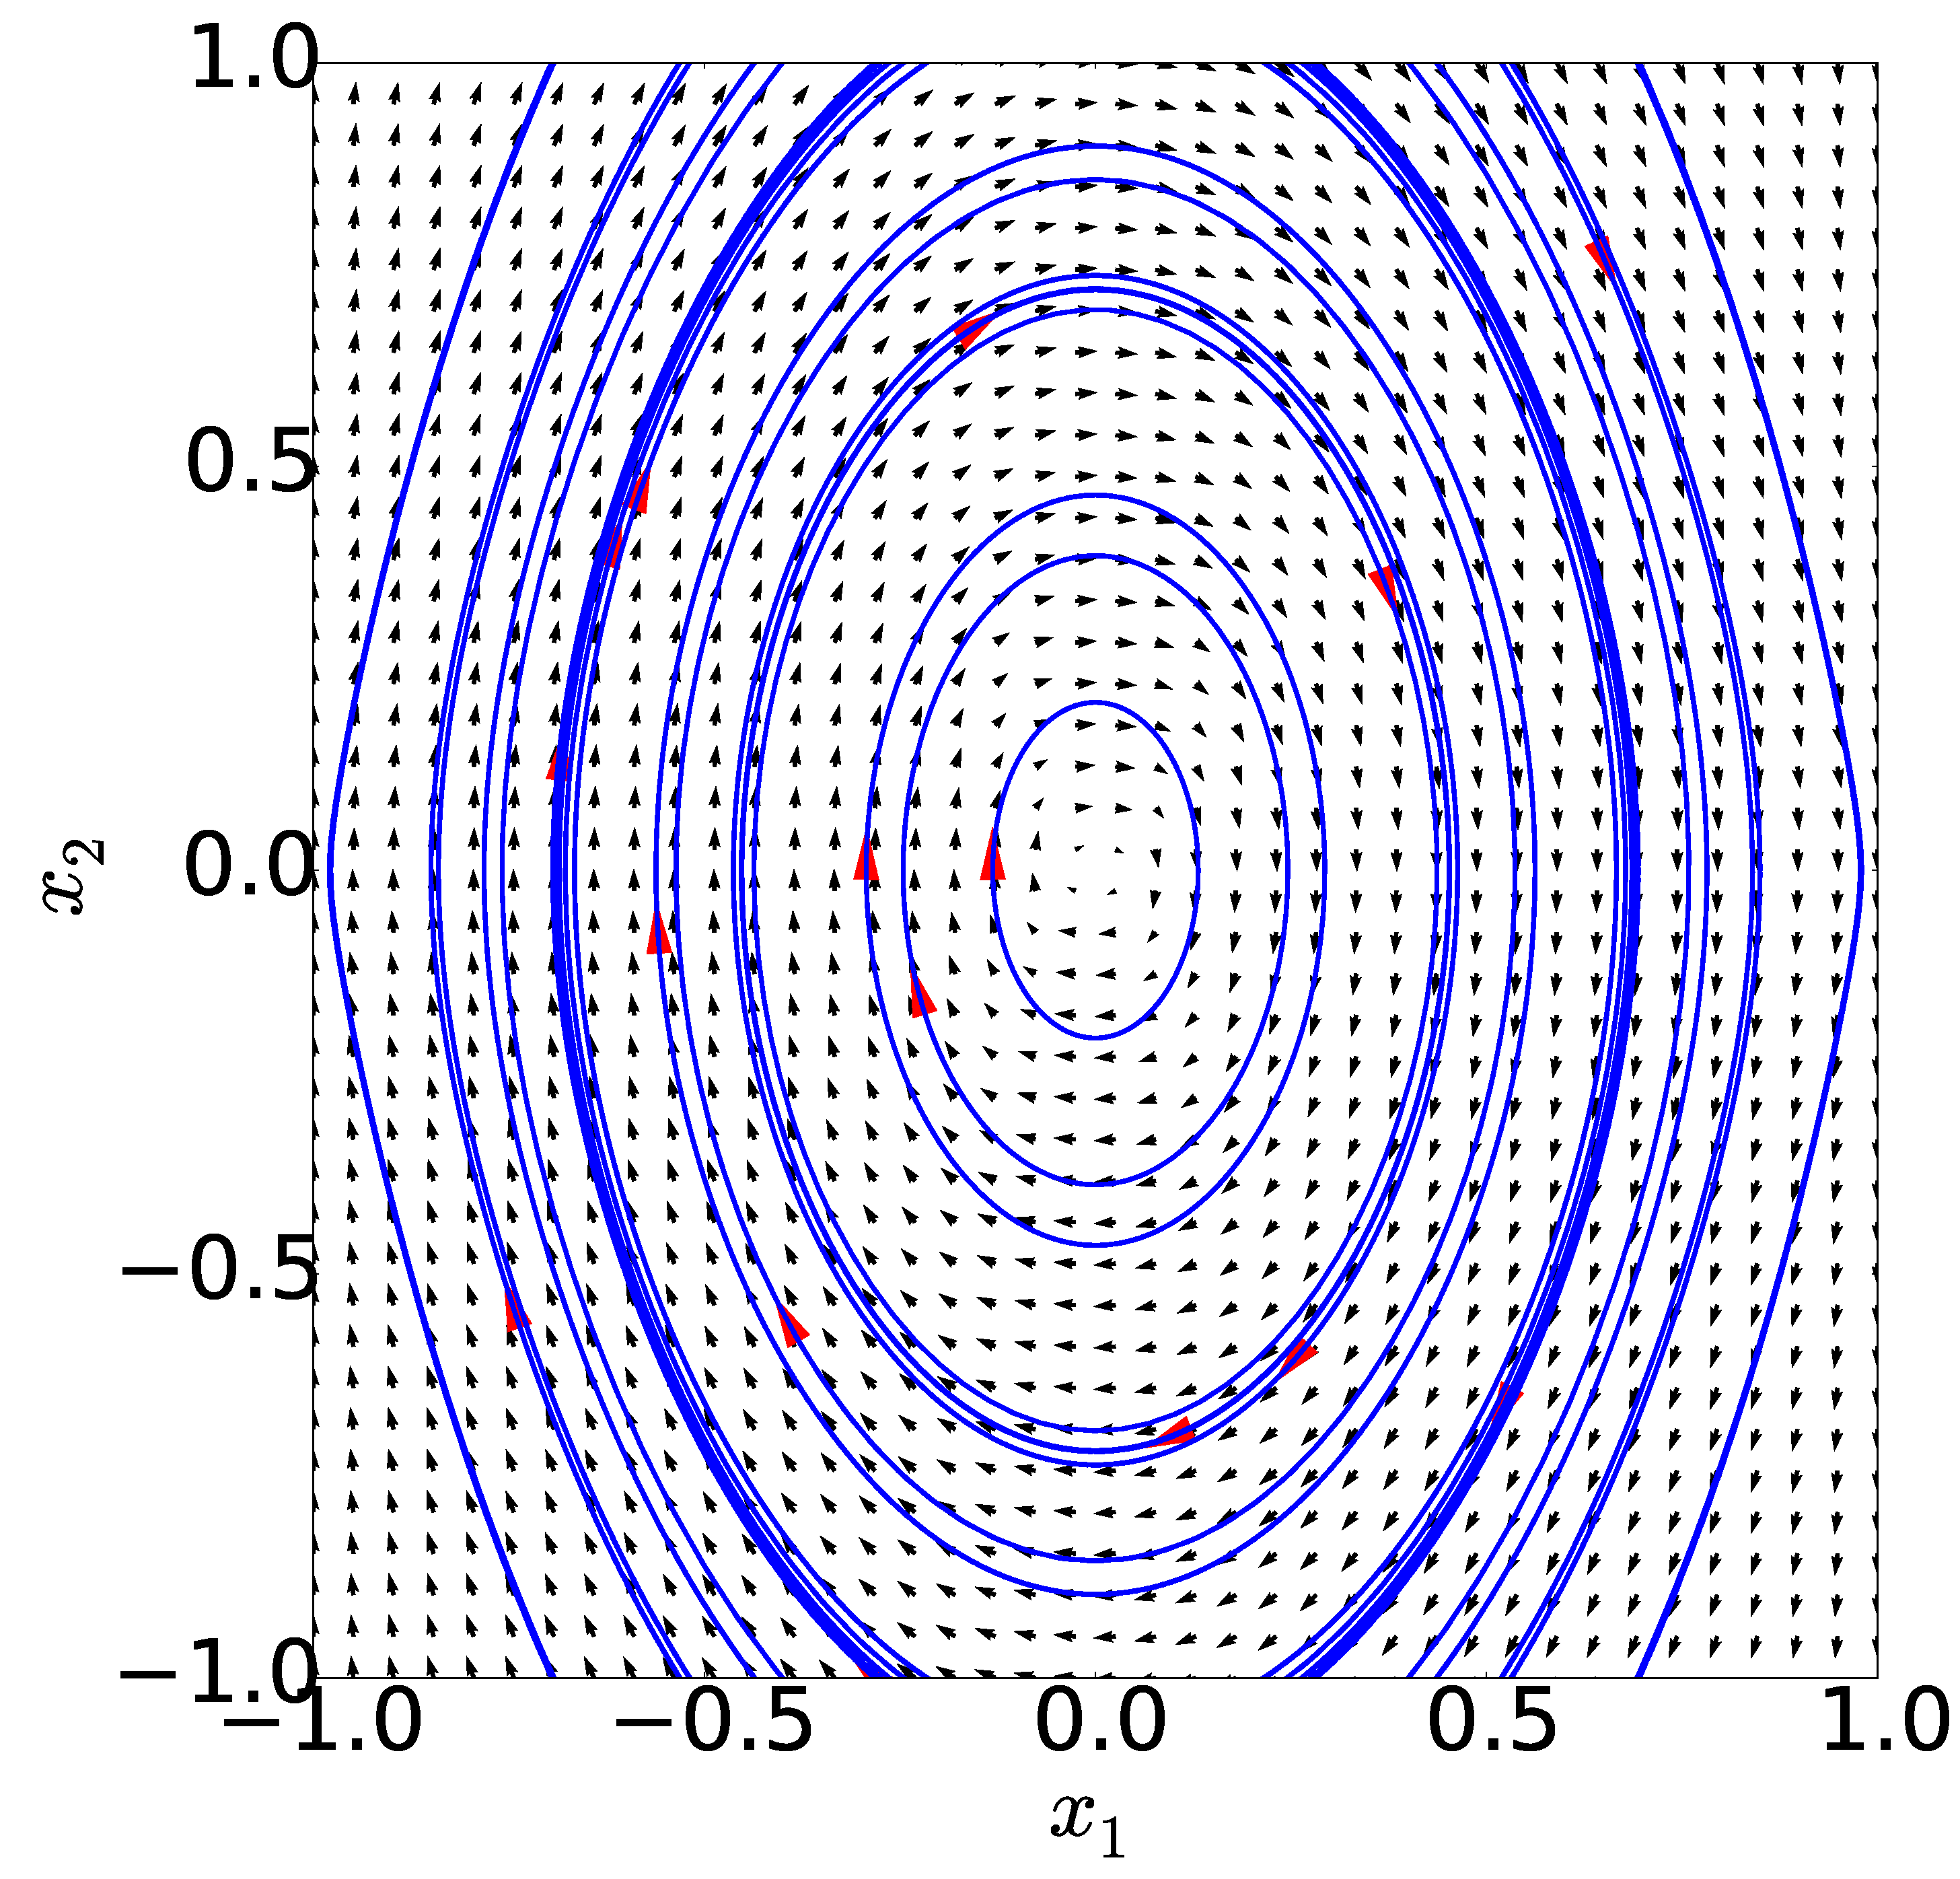
\includegraphics[width=8.0 cm]{figure/phase_portrait_2.eps}
		\caption{Case 2}
    \end{subfigure}
    \\
    \begin{subfigure}[h]{8.0 cm}
		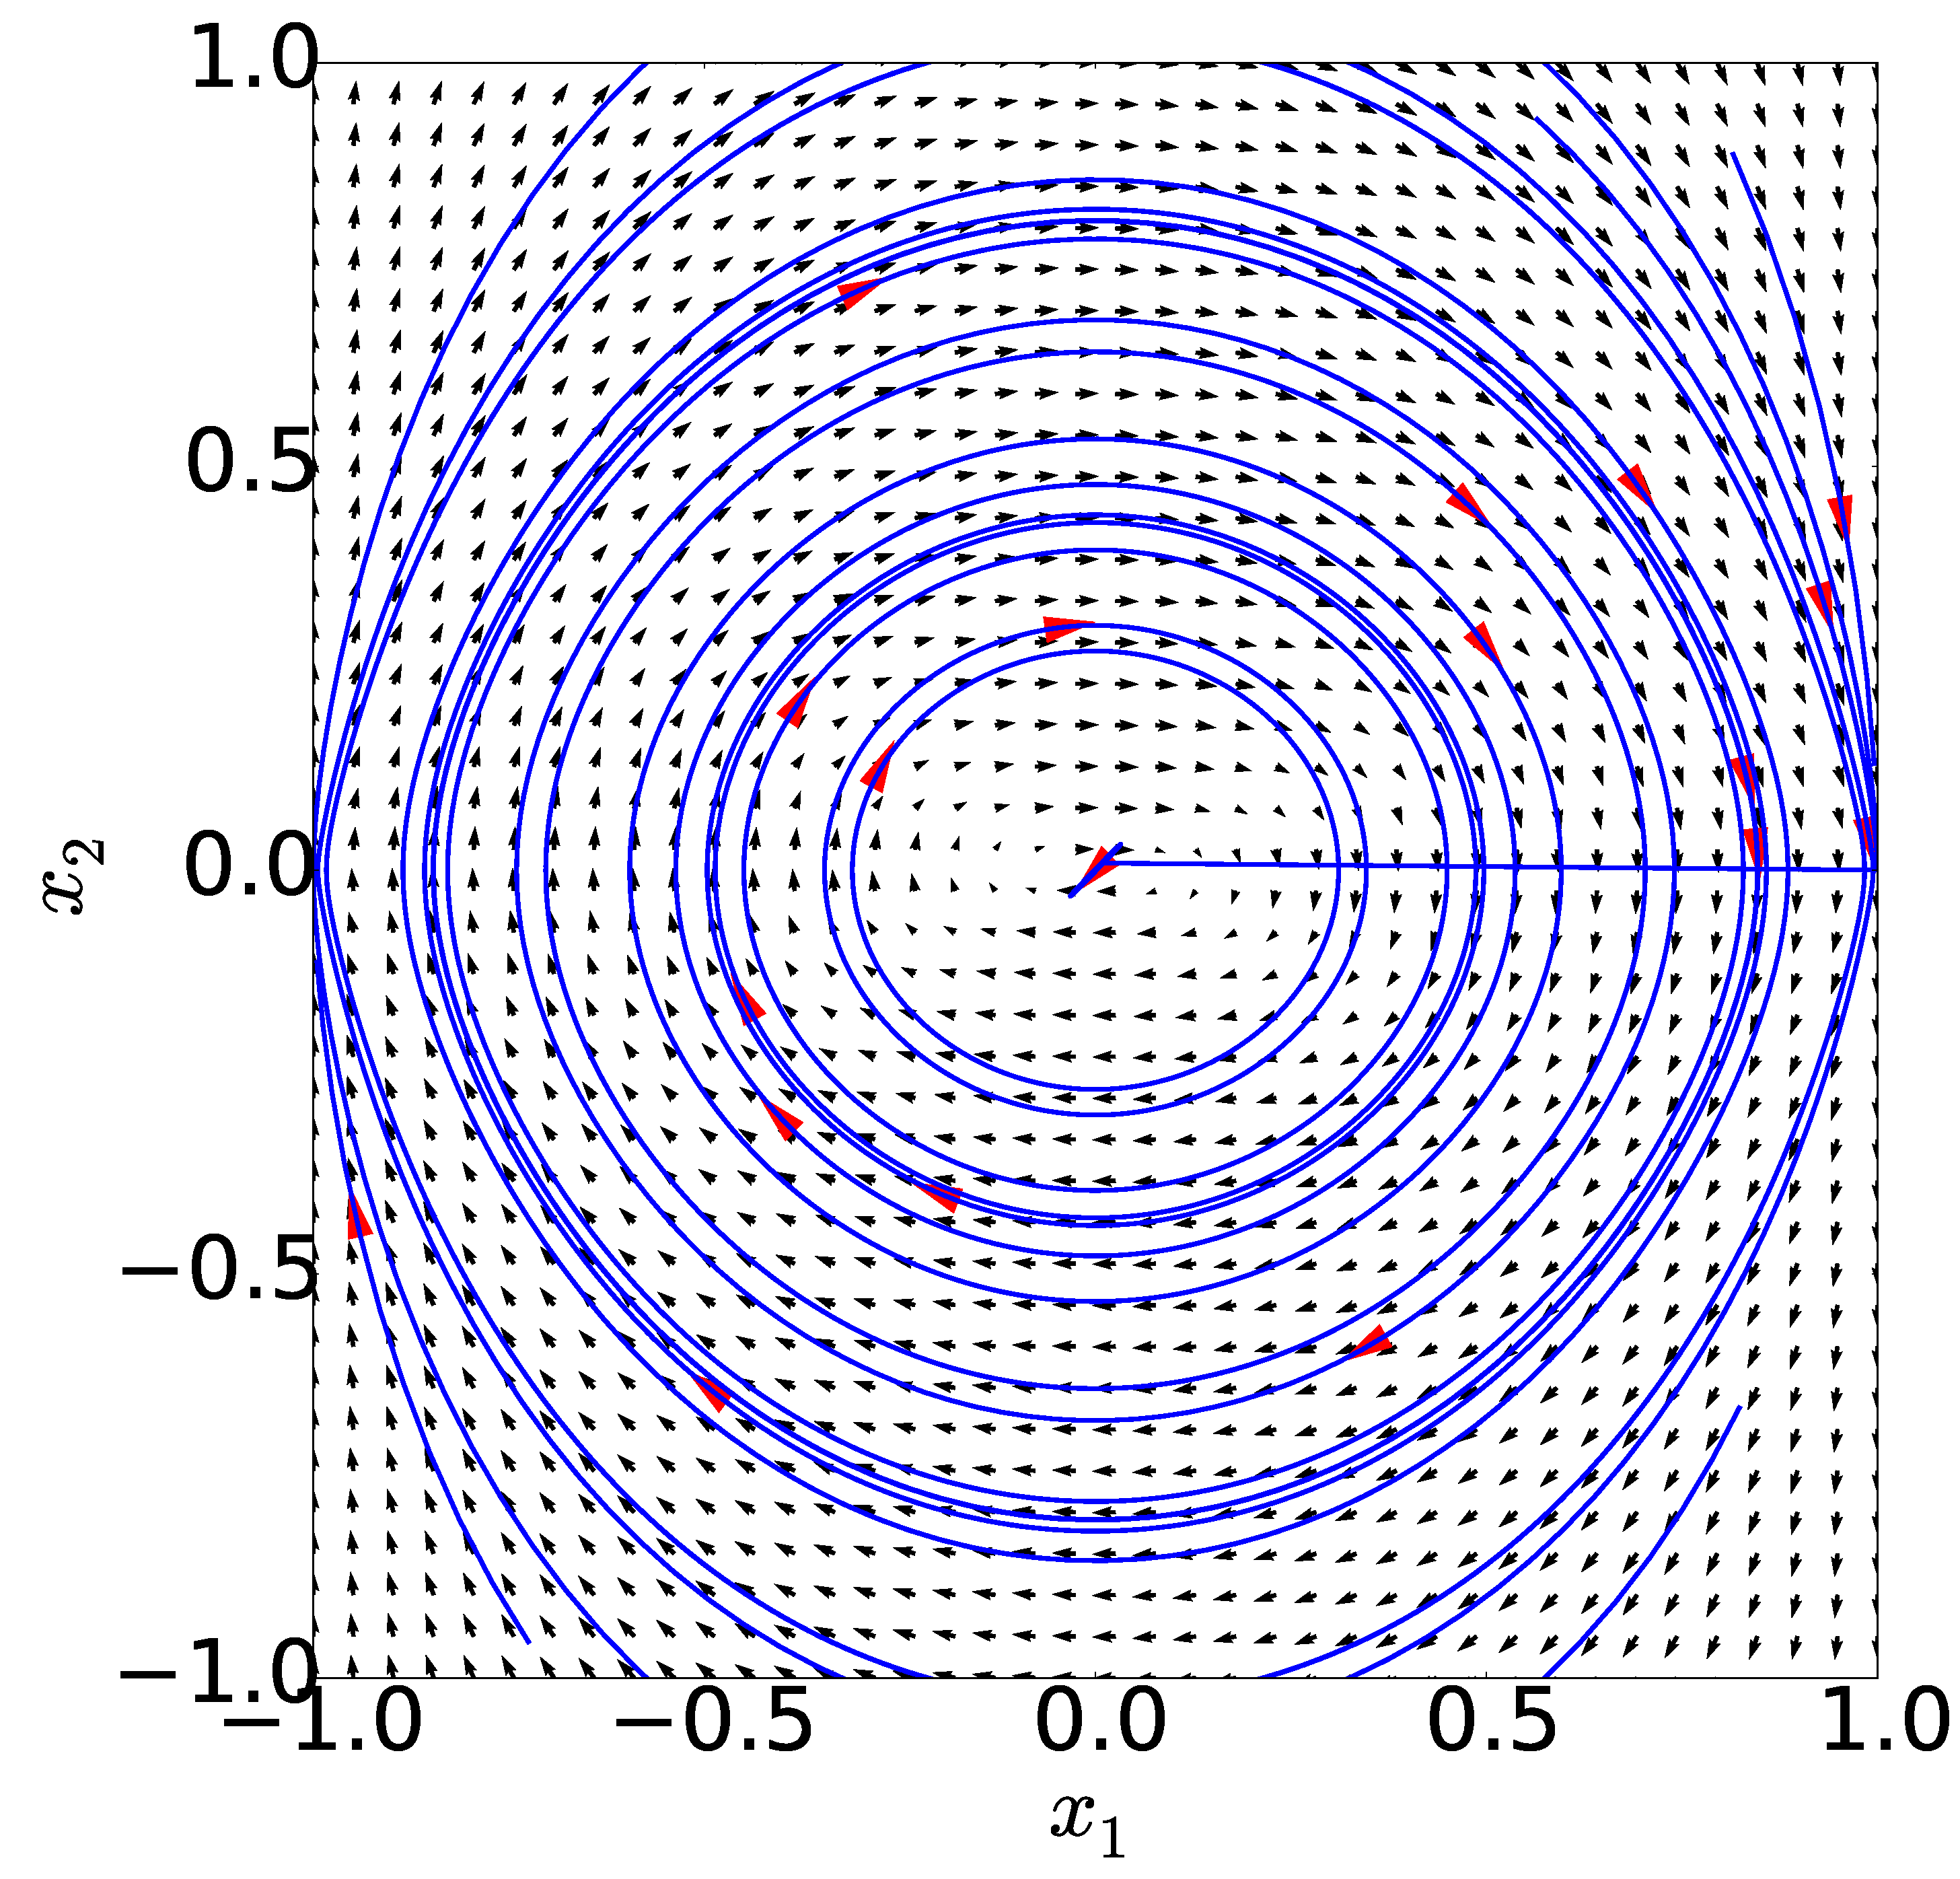
\includegraphics[width=8.0 cm]{figure/phase_portrait_3.eps}
		\caption{Case 3}
	\end{subfigure}
	\begin{subfigure}[h]{8.0 cm}
        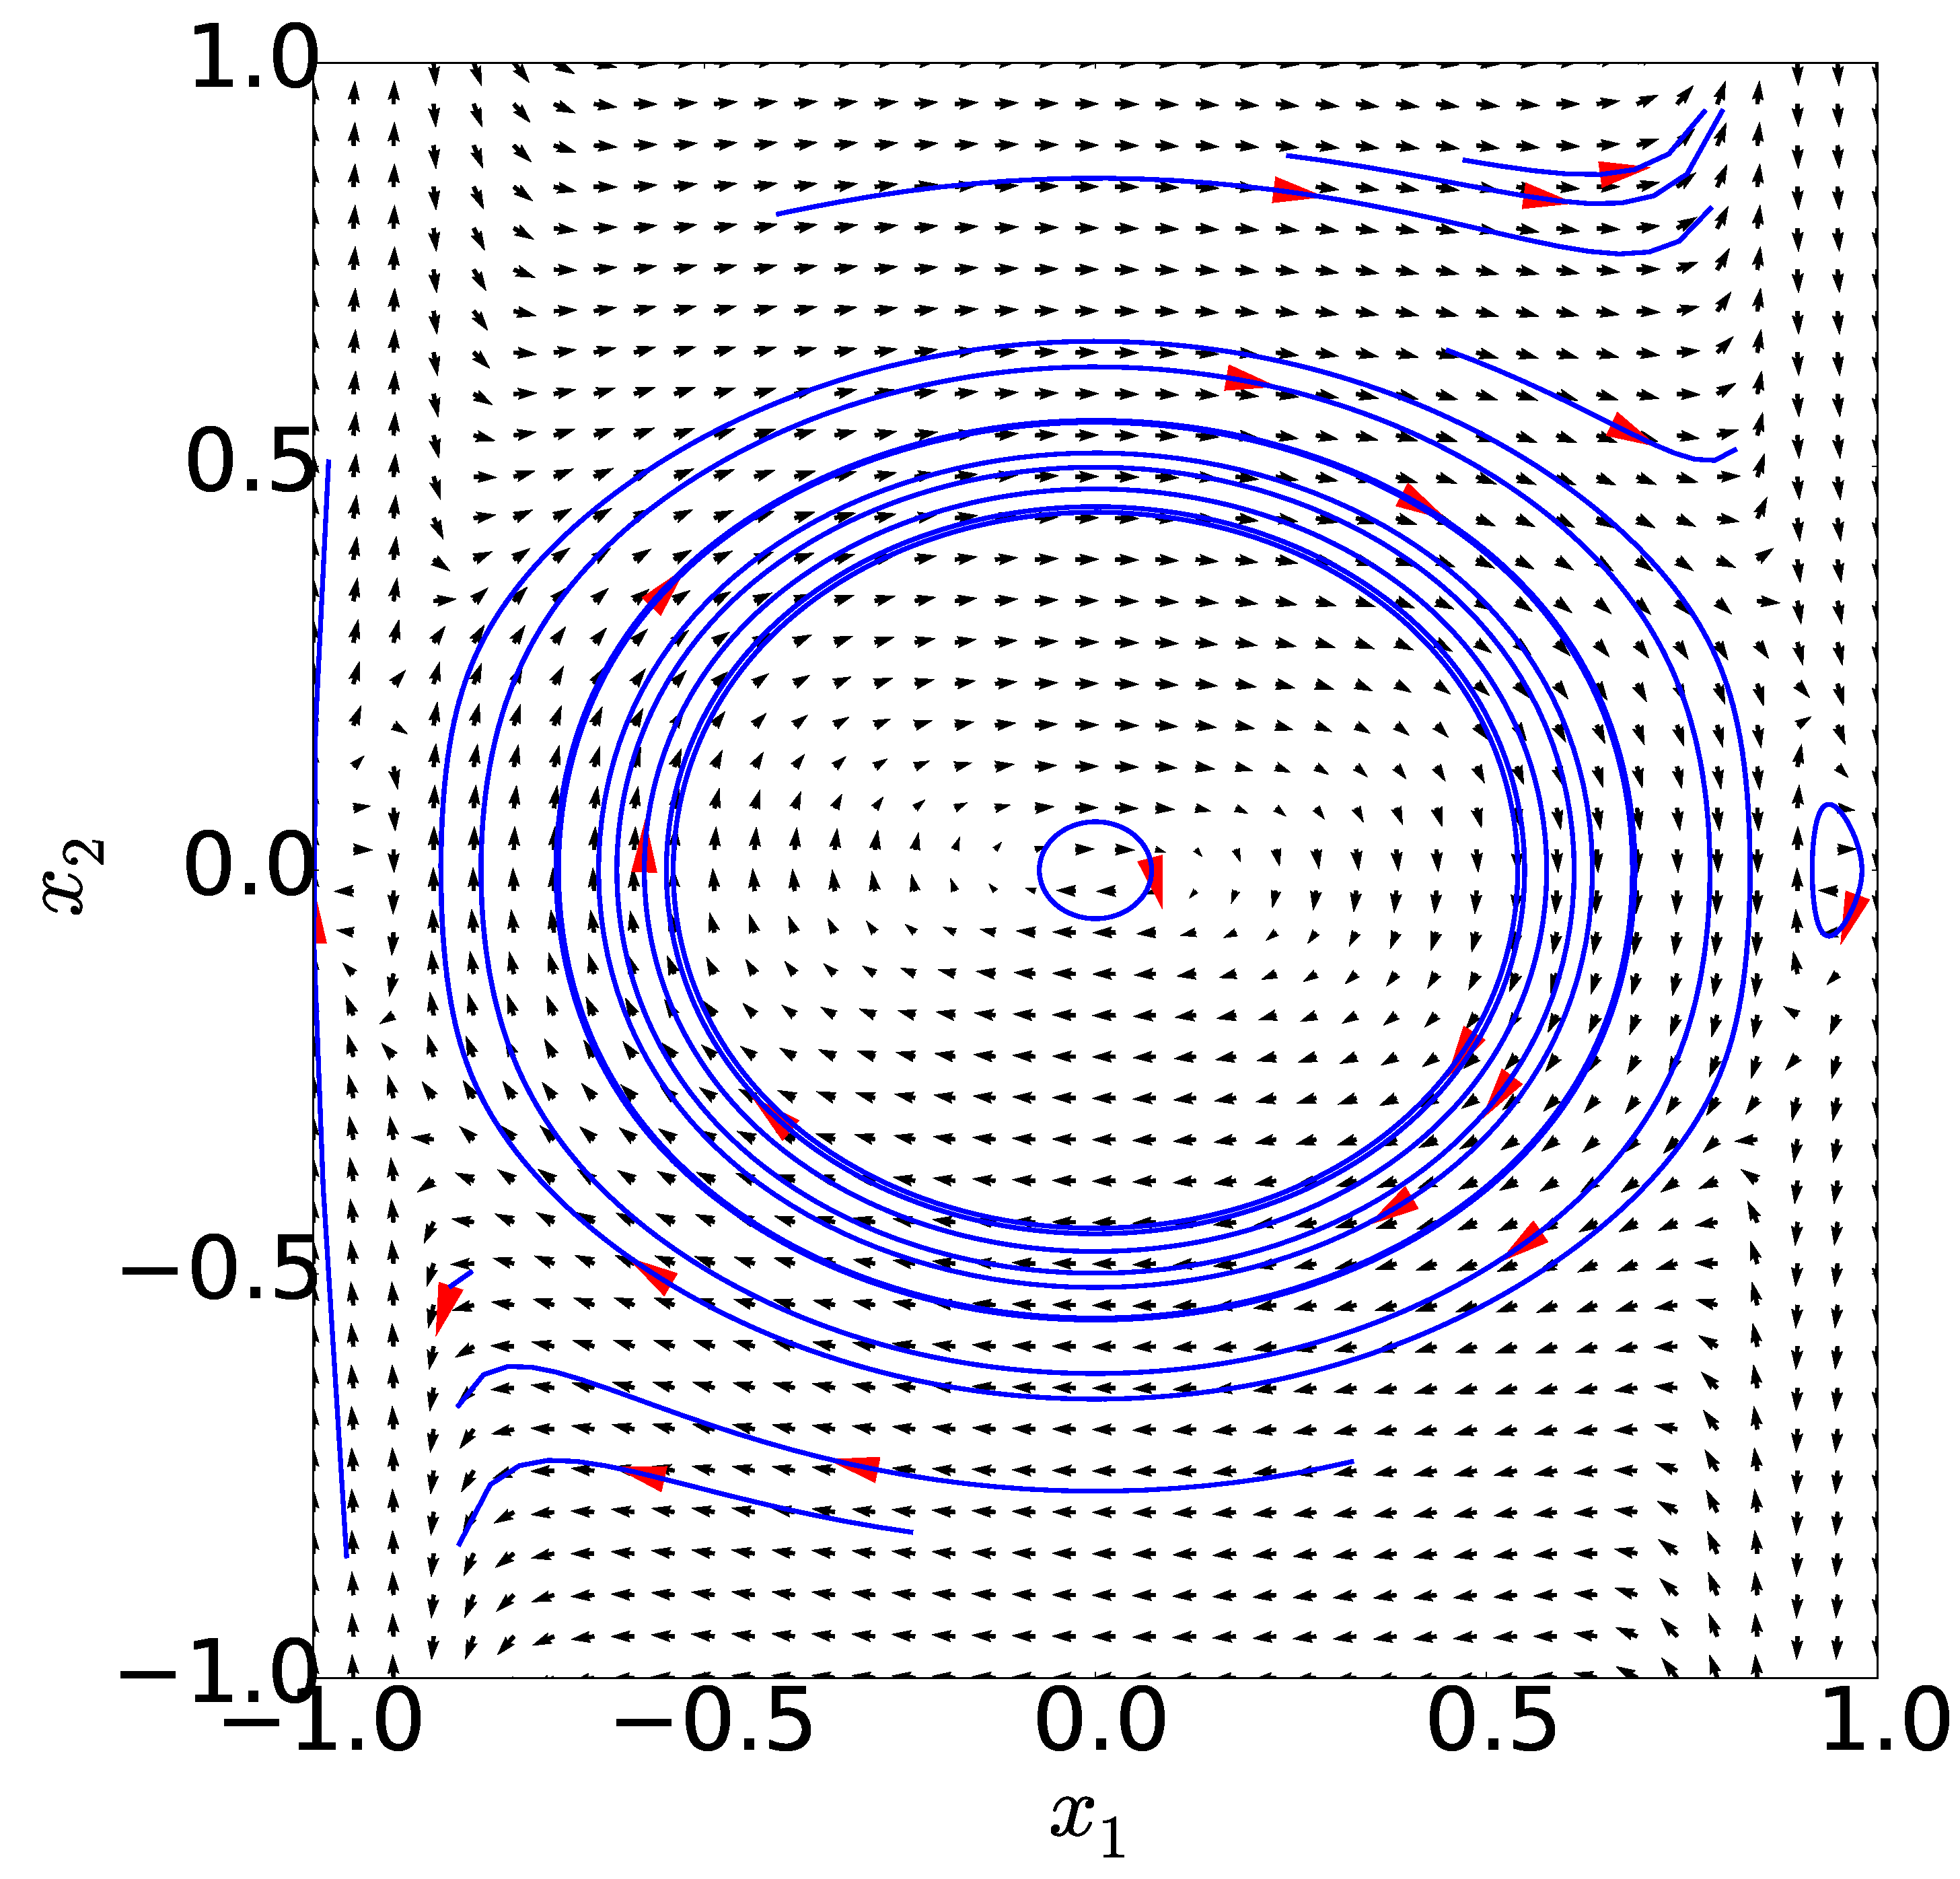
\includegraphics[width=8.0 cm]{figure/phase_portrait_4.eps}
		\caption{Case 4}
    \end{subfigure}
    \\
    	\begin{subfigure}[h]{8.0 cm}
        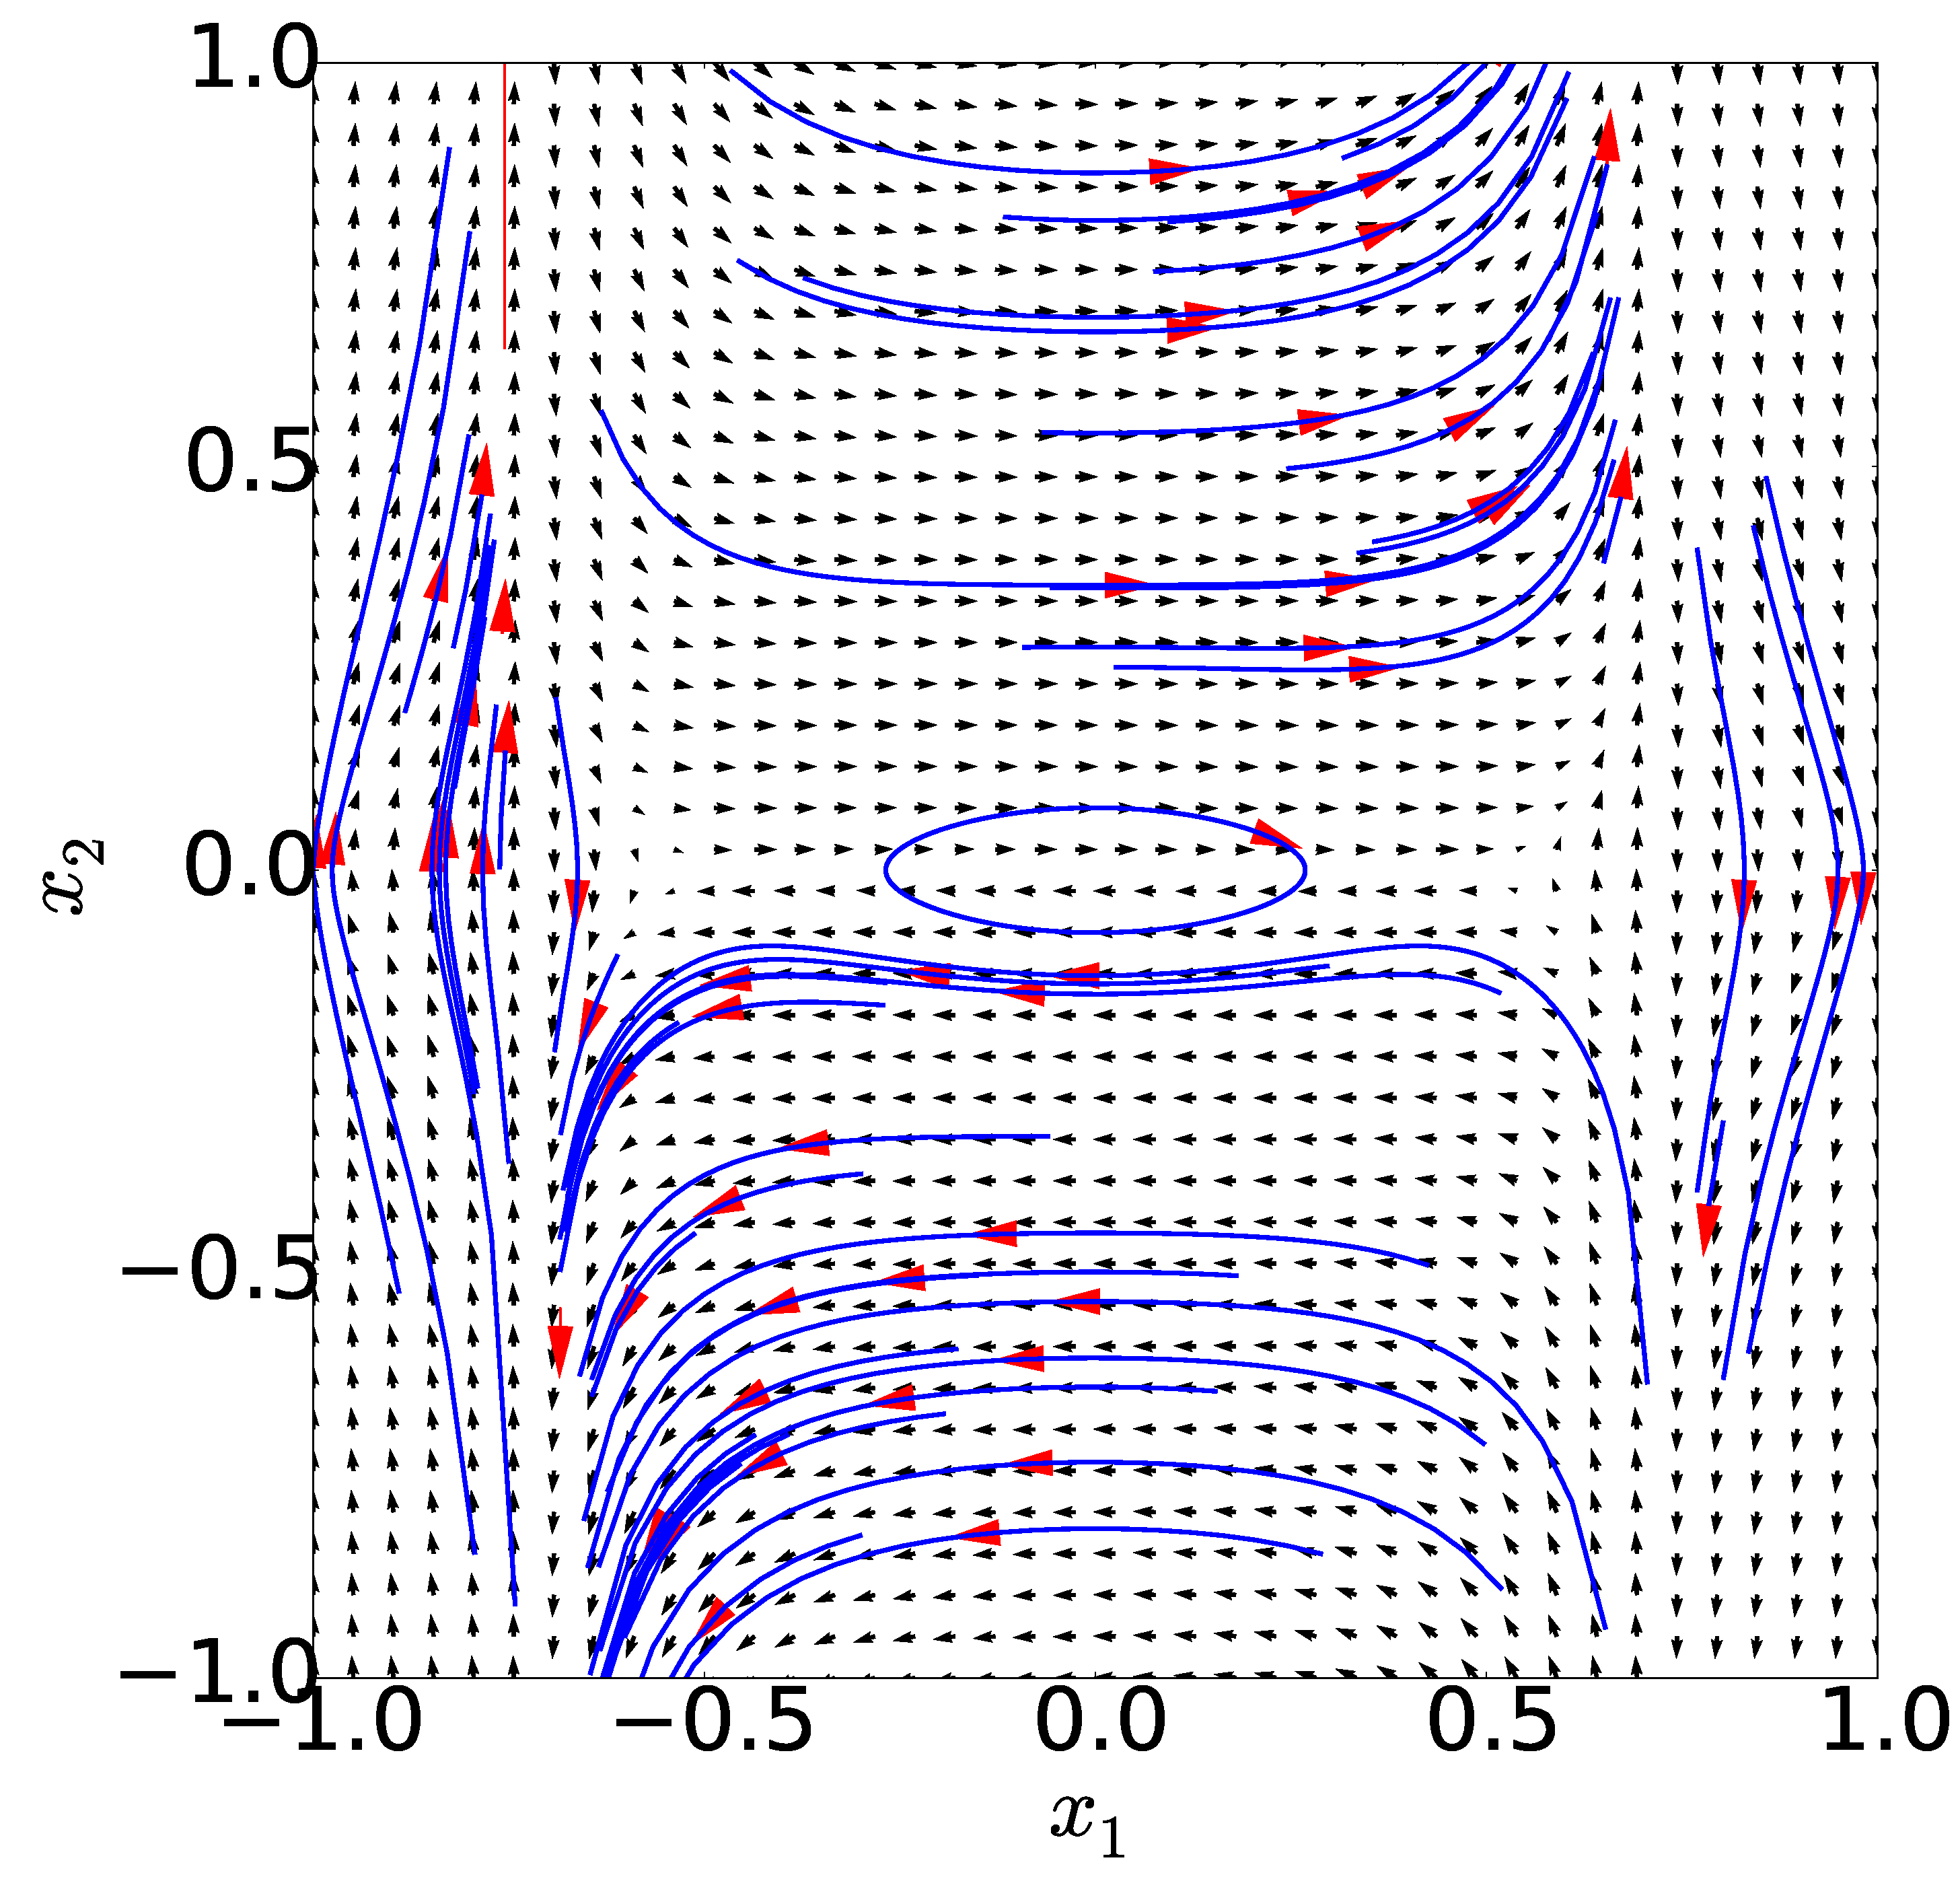
\includegraphics[width=8.0 cm]{figure/phase_portrait_5.eps}
		\caption{Case 5}
    \end{subfigure}
    	\begin{subfigure}[h]{8.0 cm}
        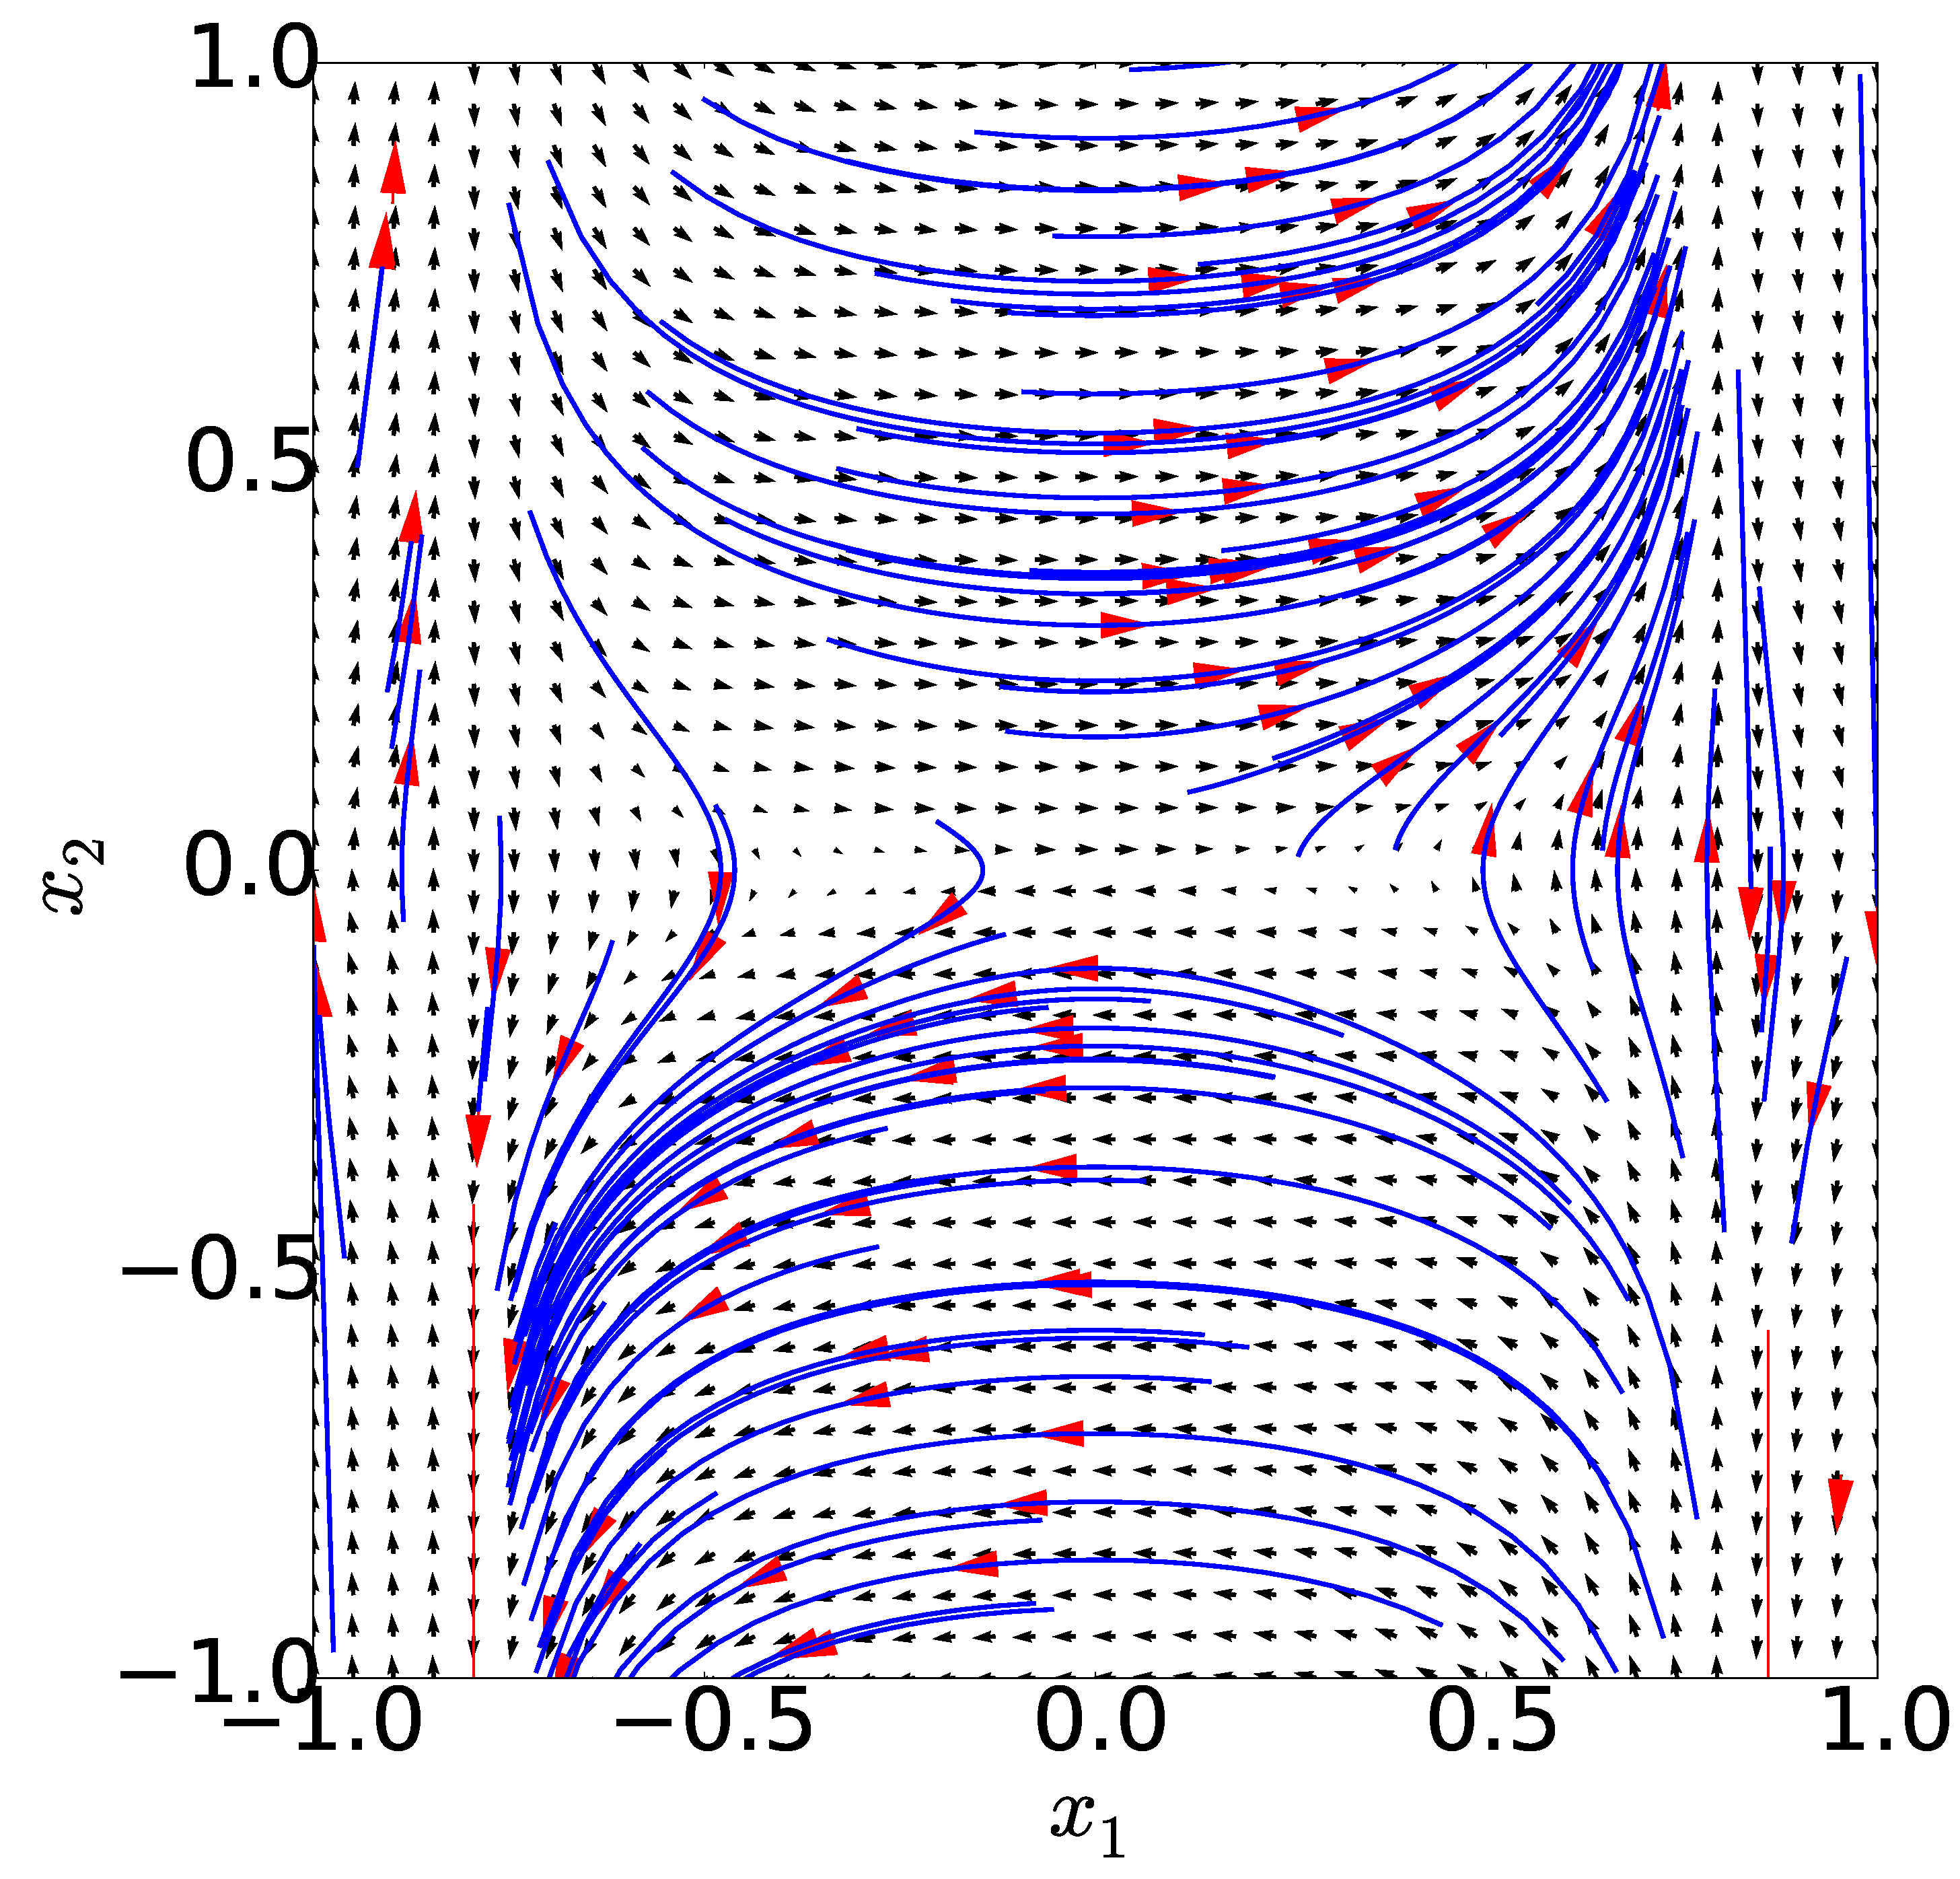
\includegraphics[width=8.0 cm]{figure/phase_portrait_6.eps}
		\caption{Case 6}
    \end{subfigure}
    \caption{Phase plot and trajectories for different values of system constants.}
    \label{fig:phasePlot}
\end{figure}

To investigate the characteristic of the stationary terms we need to look at the linearized form of the state equations.  Sign of the eigenvalues of the state matrix define the characteristic of the system.

\begin{itemize}
	\item If all the eigenvalues have negative real part, the system is asymptotically stable.
	\item If some of the eigenvalues have positive real part, the system is unstable.
	\item If some of the eigenvalues have zero real part and the rest have negative real part, system has a center point and we cannot talk about the stability of non-linear system based on the linearized form.
\end{itemize}

In the following we will look at each of the stationary points in more details.\\

\textbf{First stationary point :}$\mathbf{(x_1, x_2) = (0, 0)}:$

State Equation \eqref{eq:stateEquation} is expanded around $(0, 0)$ as shown in Equation \eqref{eq:StateEquationAt0}. By only keeping the linear terms, the state equation can be rewritten in the matrix form as follows

\begin{equation}
	\begin{bmatrix}
	\dot{y}_1 \\
	\dot{y}_2
	\end{bmatrix} = 
	\begin{bmatrix}
	0 & 1 \\
	- \dfrac{\epsilon}{l} g - \dfrac{k}{m_{1}} & 0
	\end{bmatrix}
	\begin{bmatrix}
	y_1 \\
	y_2
	\end{bmatrix}
\end{equation}

The eigenvalues of this matrix can be written as

\begin{equation}
	\pm \sqrt{- \dfrac{\epsilon}{l} g - \dfrac{k}{m_{1}}}
\end{equation}

Based on the sign of $- \dfrac{\epsilon}{l} g - \dfrac{k}{m_{1}}$ we will have three cases.

\begin{itemize}
	\item If $- \dfrac{\epsilon}{l} g - \dfrac{k}{m_{1}} > 0$ then we have two real eigenvalues with different signs. Therefore, the system becomes unstable.
	\item If $- \dfrac{\epsilon}{l} g - \dfrac{k}{m_{1}} < 0$ then we have two imaginary eigenvalues with zero real parts. Therefore, the fixed point is a center and linearization cannot determine the stability of this fixed point.
	\item if $- \dfrac{\epsilon}{l} g - \dfrac{k}{m_{1}} = 0$ then both of the eigenvalues are zero and we have rigid body motion of the system.
\end{itemize}

Figure \ref{fig:PhasePlotExpanded0} shows the phase plot of expanded state equation around $(0, 0)$ for different cases of system constants defined in Table \ref{table:systemConstantsExpanded0}.

\begin{table}[htbp]
\begin{center}
\begin{tabular}{c||c|c|c|c|c|c}
case number & $\epsilon$ & $k$ & $m_1$ & $g$ & $l$ & $\dfrac{-\epsilon}{l}g - \dfrac{k}{m_1}$ \\ \hline \hline
1 & 0.1 & 1 & 1 & 1 & 1 & -1.1 \\ \hline
2 & -1.5 & 1 & 1.6 & 1 & 1 & 0.875 \\ \hline
3 & -1 & 2 & 1 & 2 & 1 & 0 \\
\end{tabular}
\end{center}
\caption{System constants}
\label{table:systemConstantsExpanded0}
\end{table}

\begin{figure}[H]
	\centering
	\begin{subfigure}[h]{8.0 cm}
		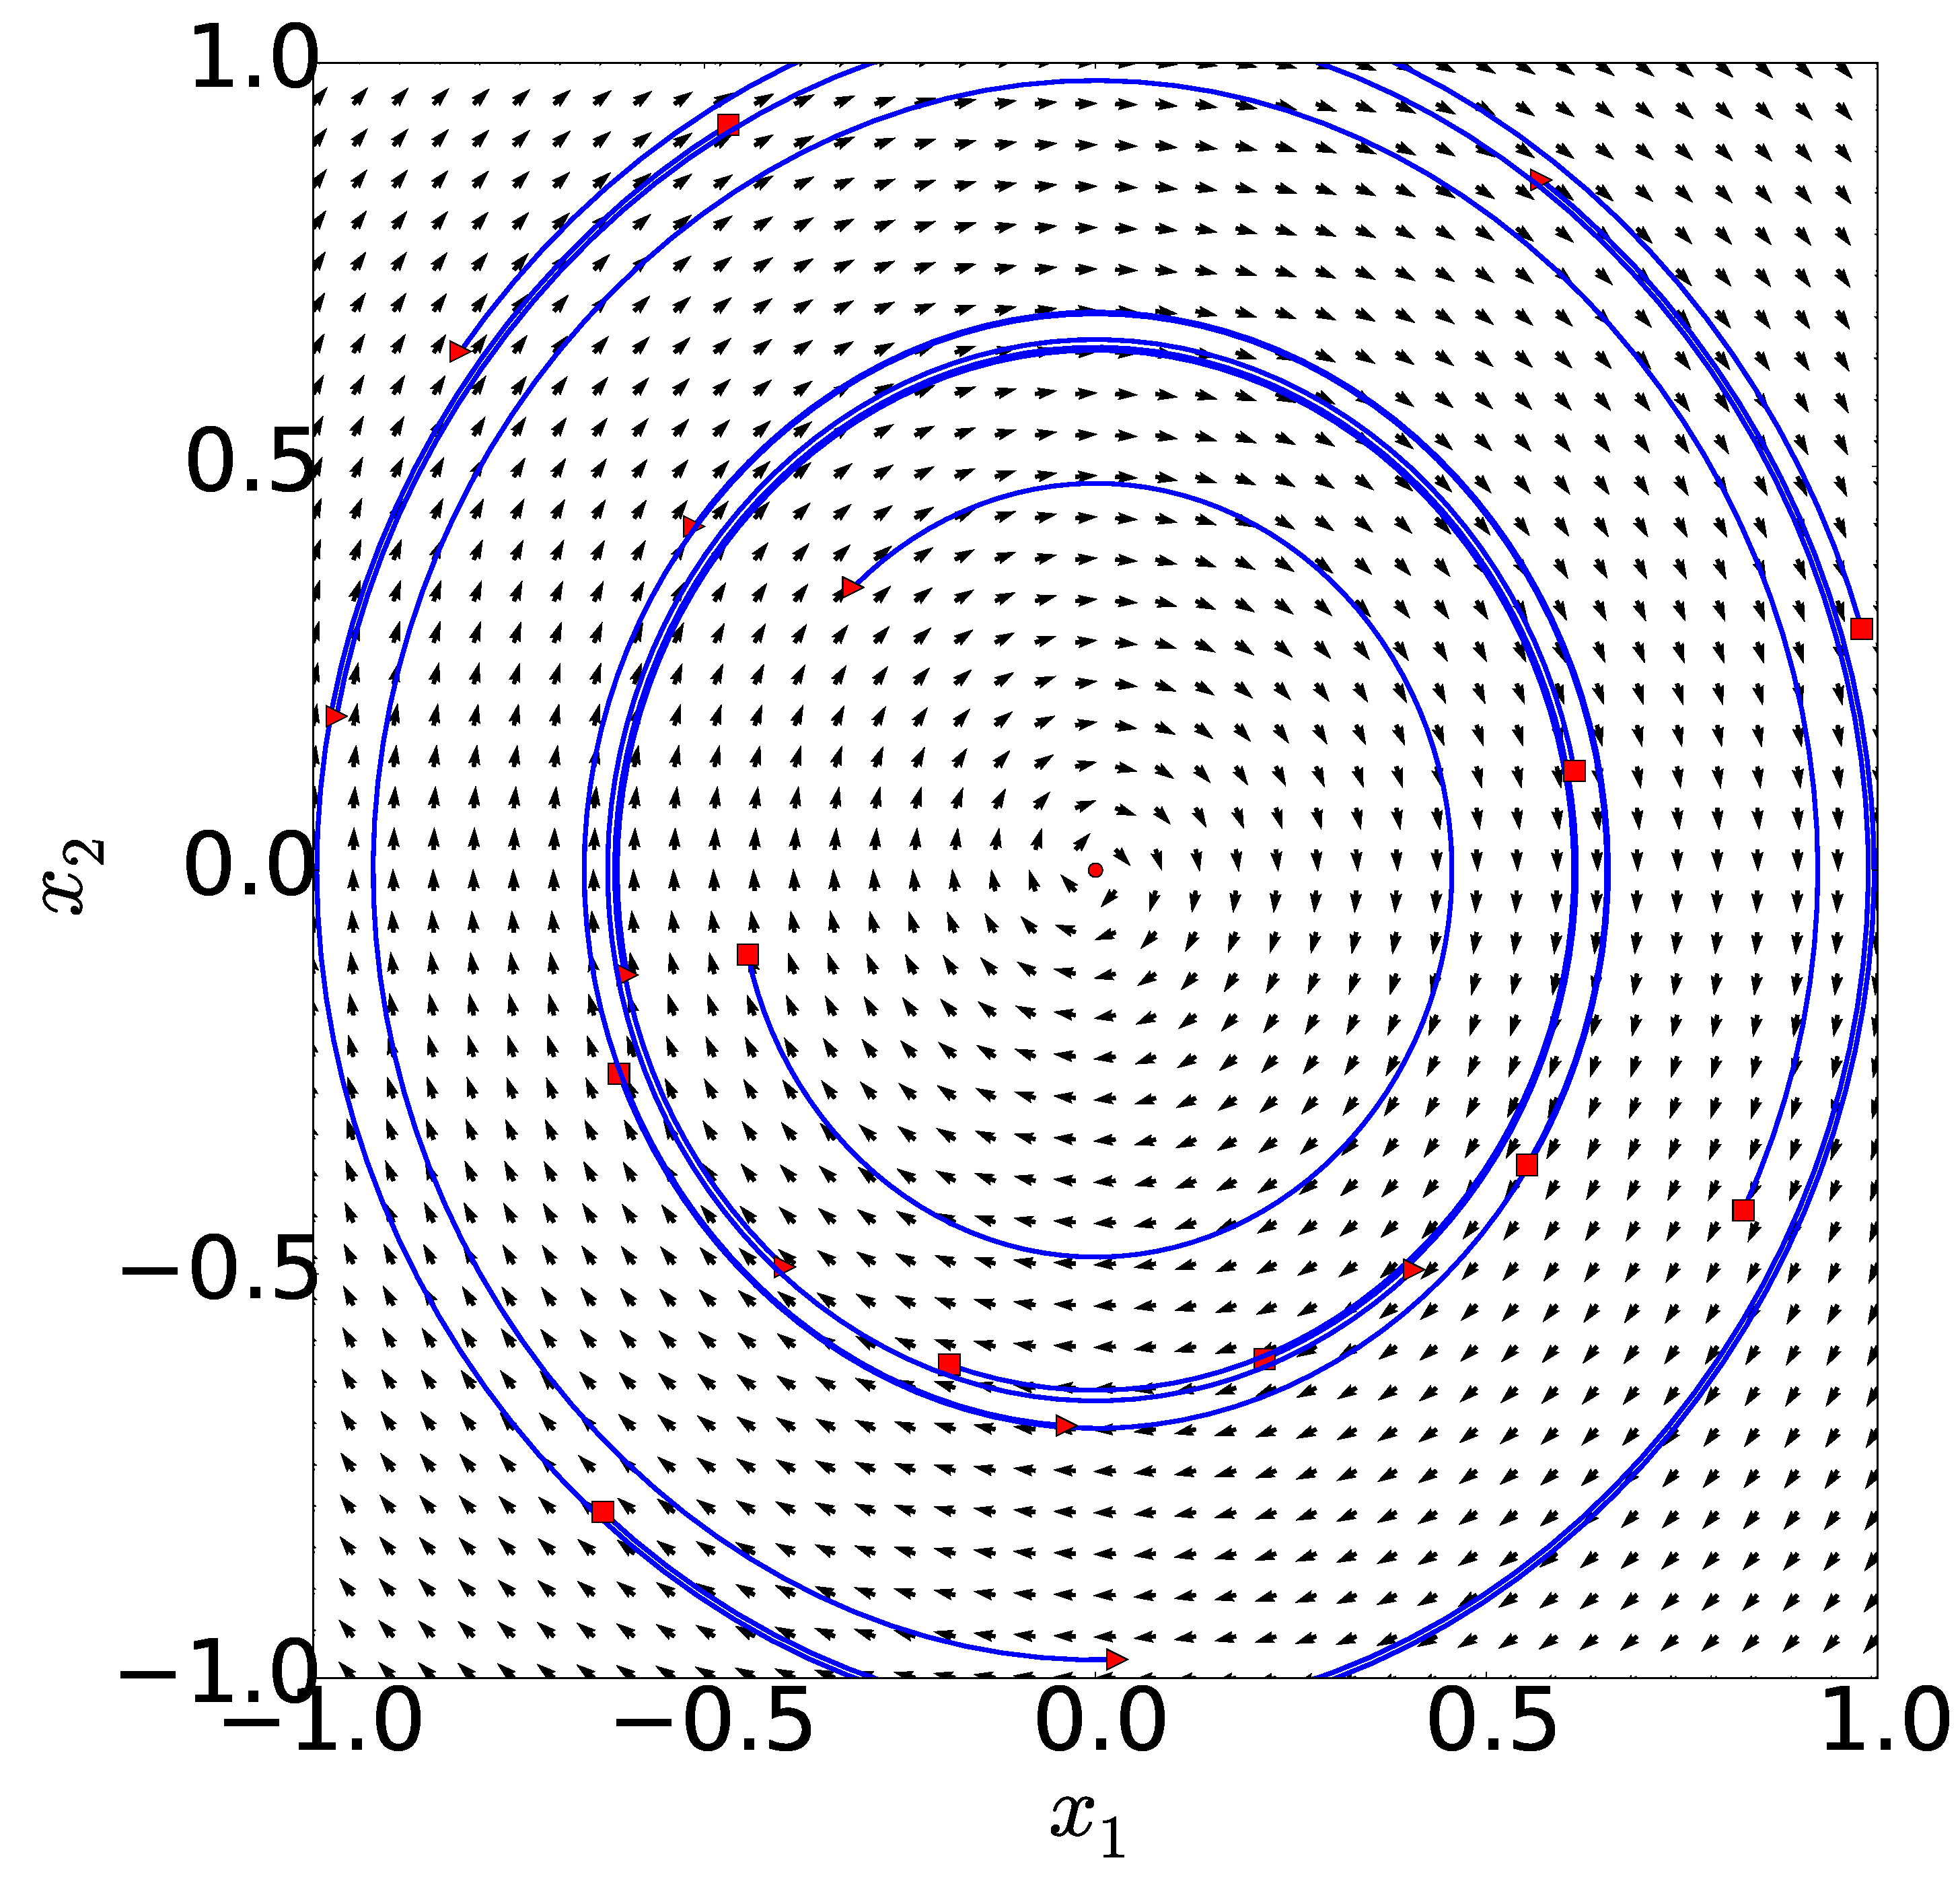
\includegraphics[width=8.0 cm]{figure/phase_portrait_around_x10_00_x20_0_1.eps}
		\caption{Case 1 - Expanded function}
	\end{subfigure}
	\begin{subfigure}[h]{8.0 cm}
        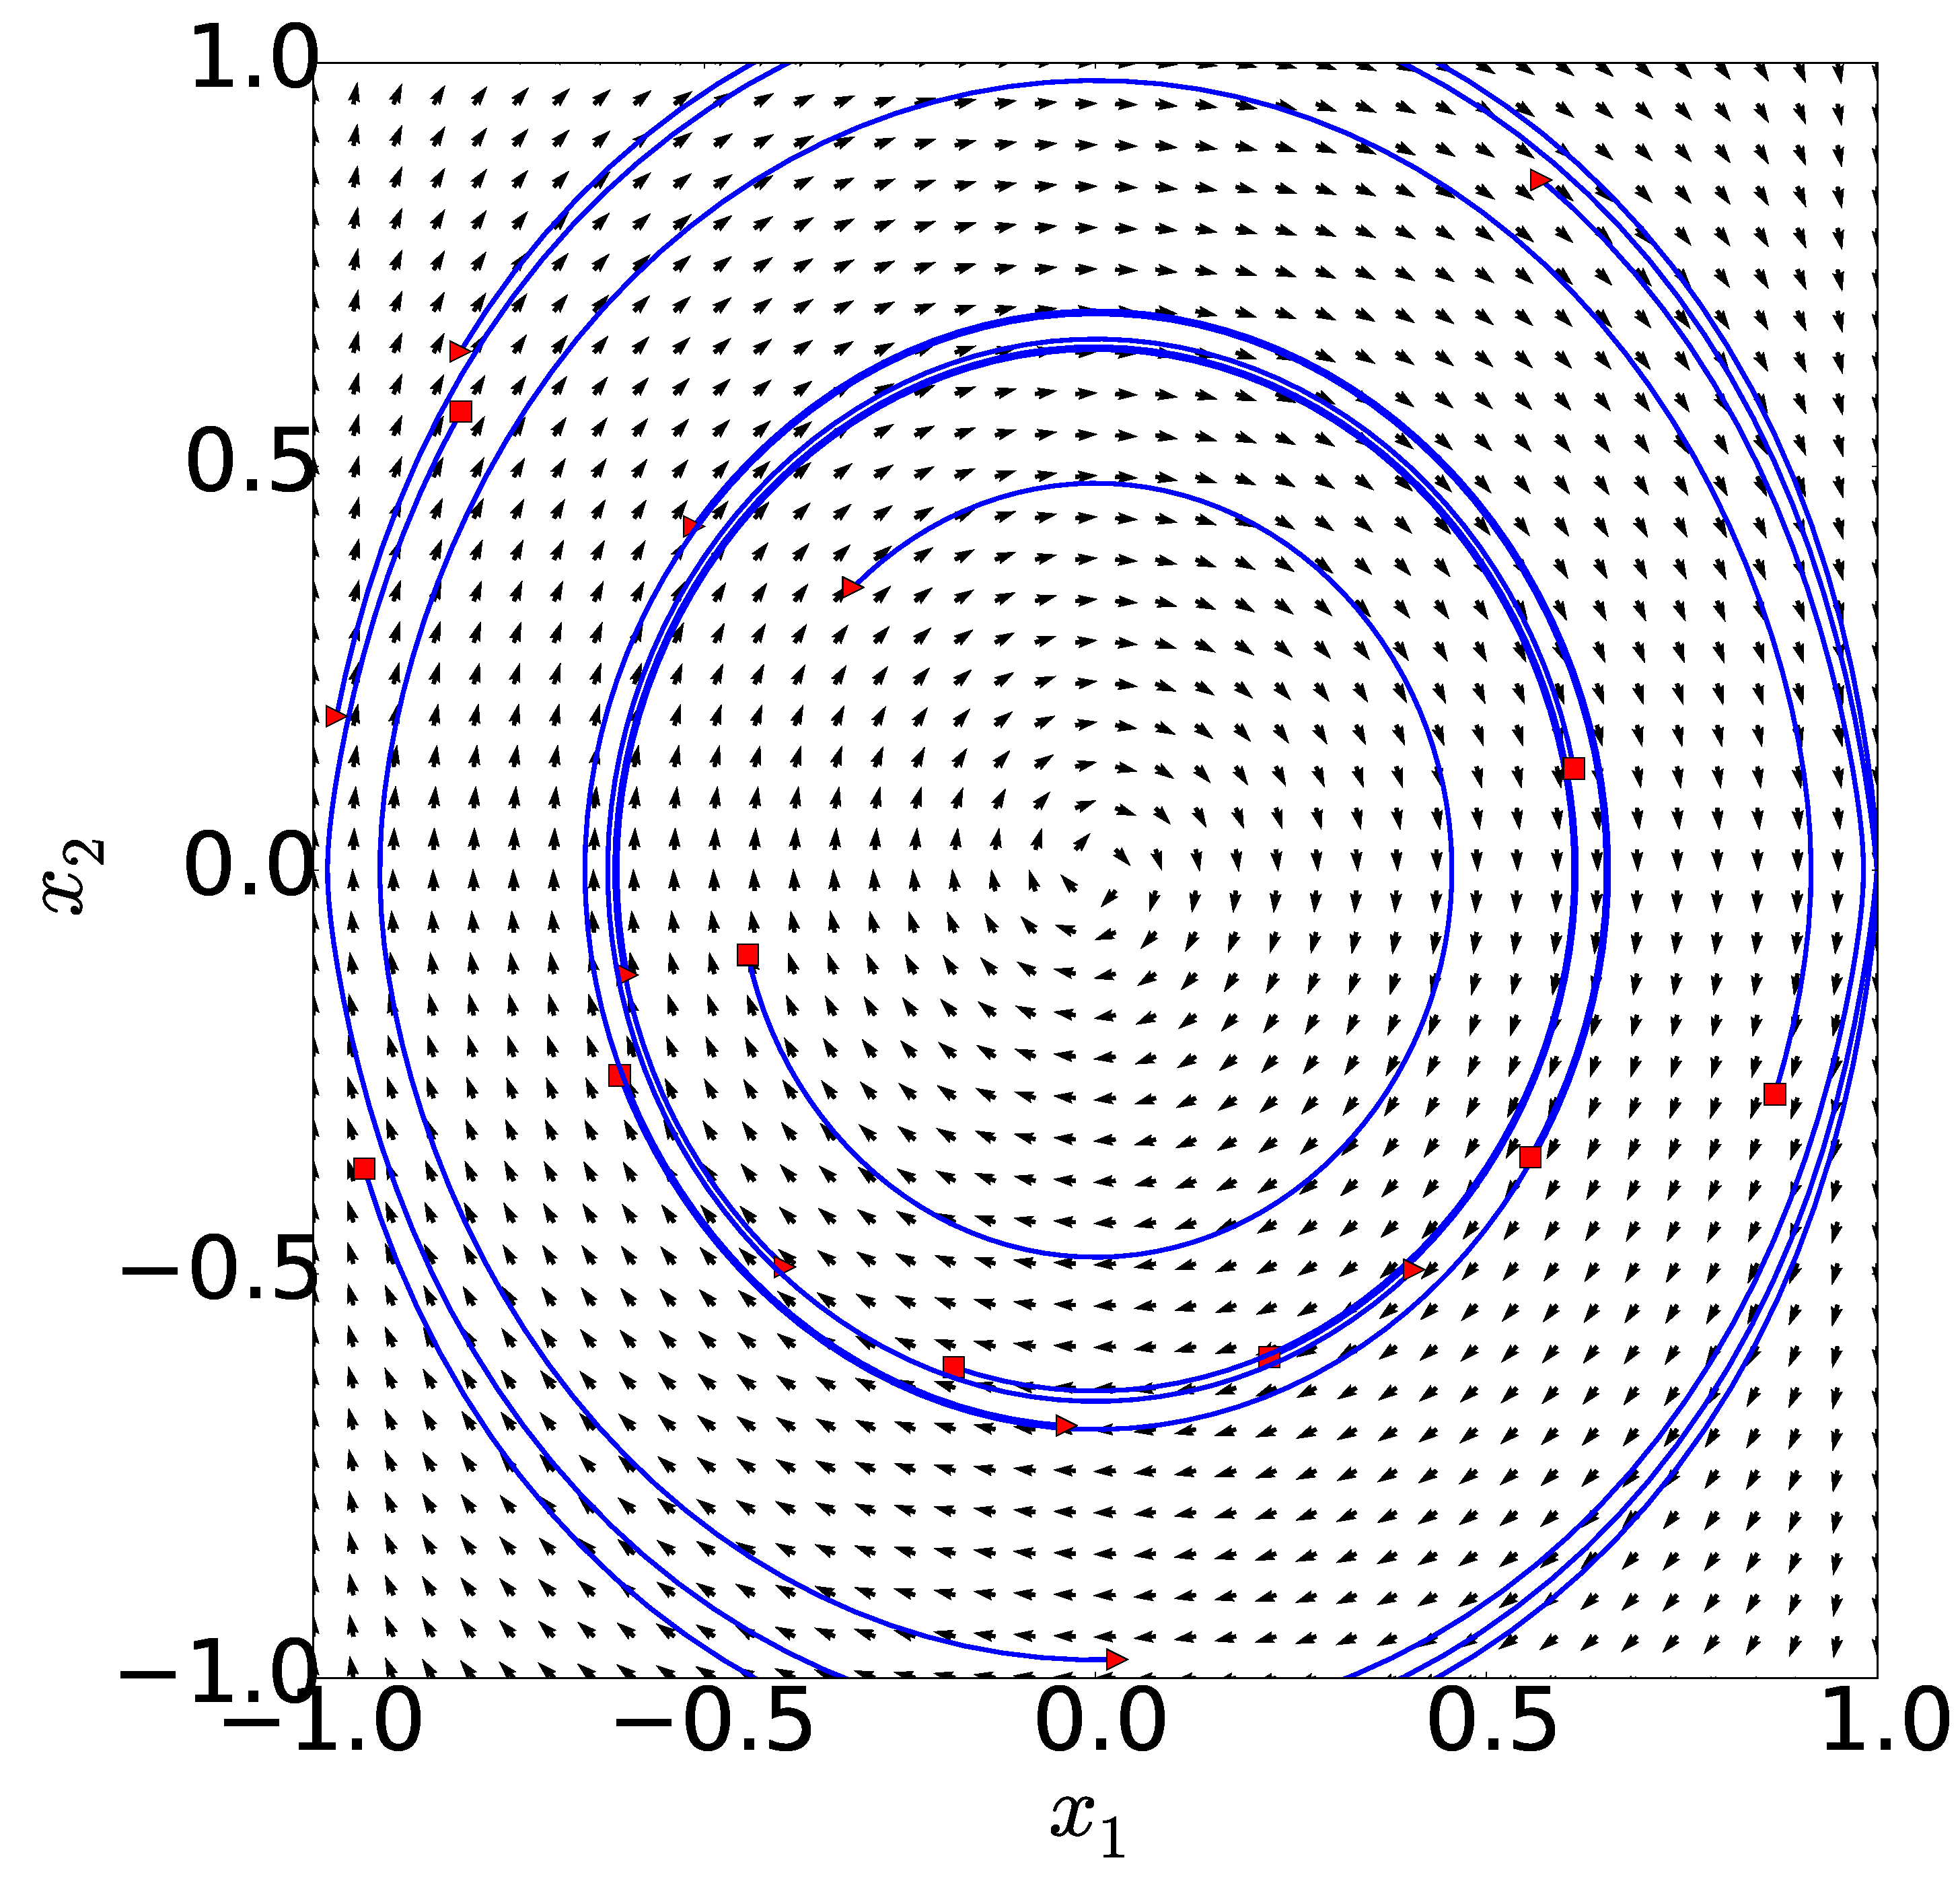
\includegraphics[width=8.0 cm]{figure/phase_portrait_l2nlcomp1.eps}
		\caption{Case 1 - Actual function}
    \end{subfigure}
    \\
    \begin{subfigure}[h]{8.0 cm}
		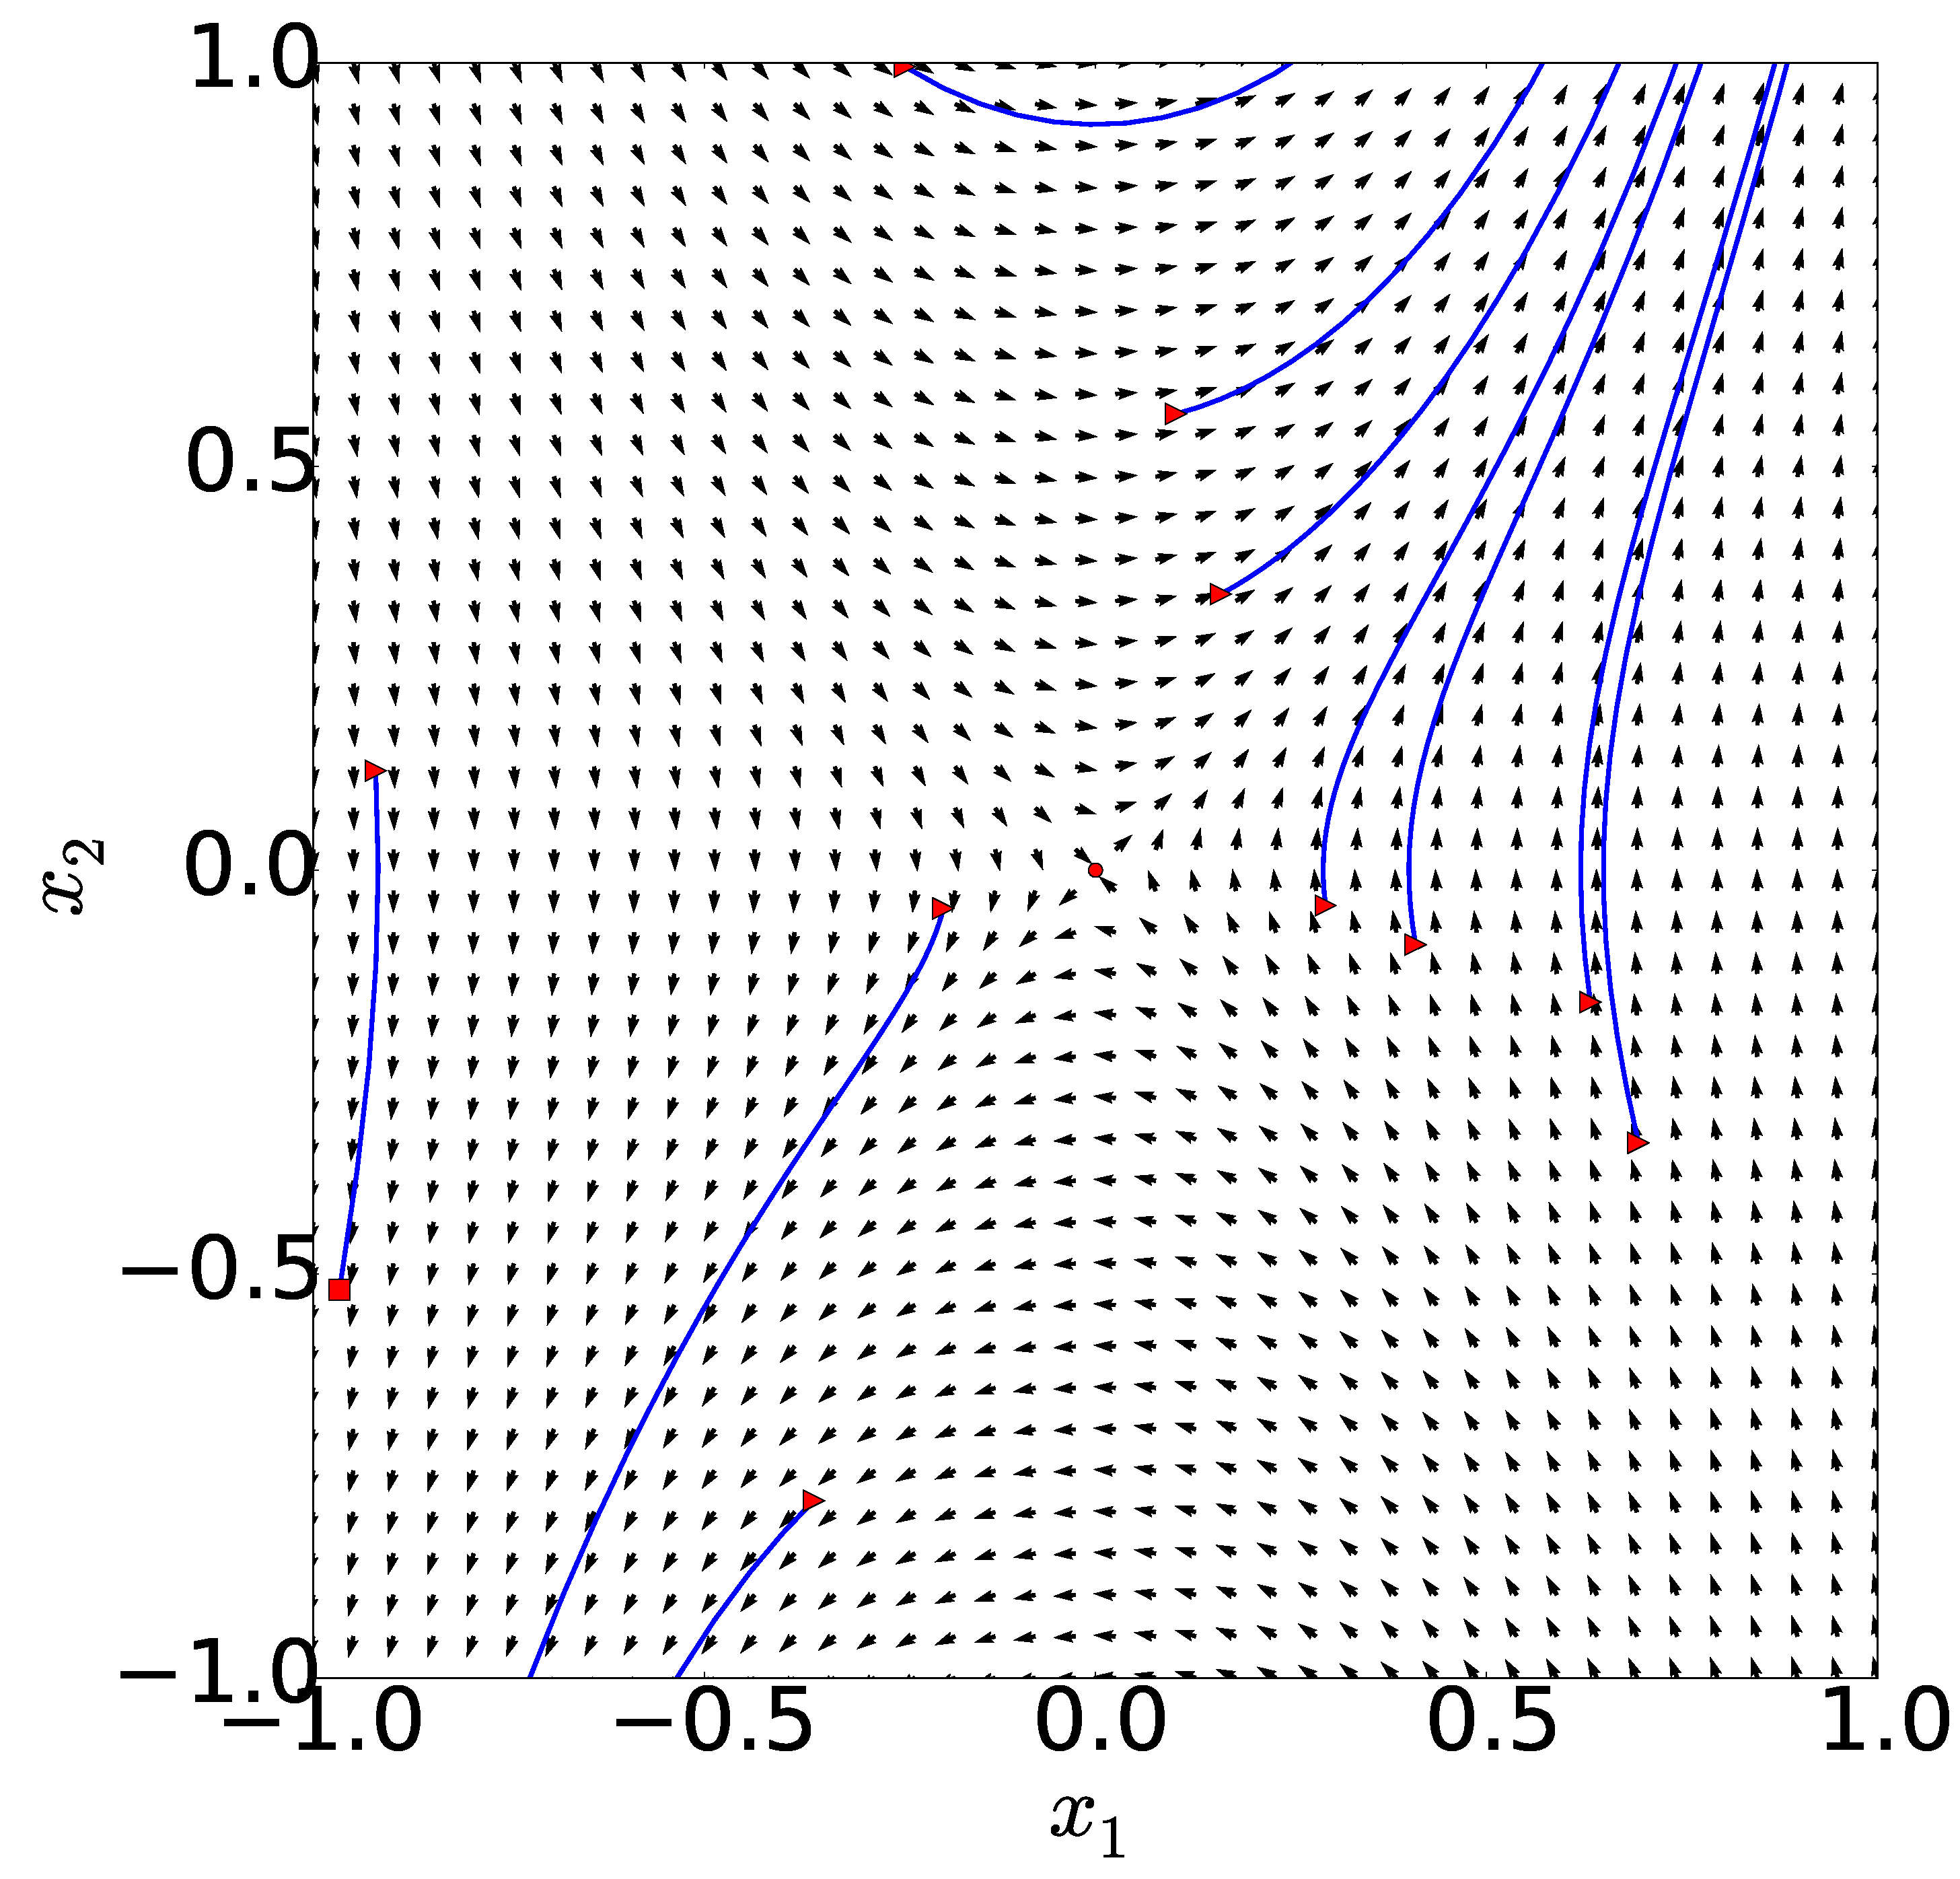
\includegraphics[width=8.0 cm]{figure/phase_portrait_around_x10_00_x20_0_2.eps}
		\caption{Case 2 - Expanded function}
	\end{subfigure}
	\begin{subfigure}[h]{8.0 cm}
        \includegraphics[width=8.0 cm]{figure/phase_portrait_l2nlcomp2.eps}
		\caption{Case 2 - Actual function}
    \end{subfigure}
    \\
    	\begin{subfigure}[h]{8.0 cm}
        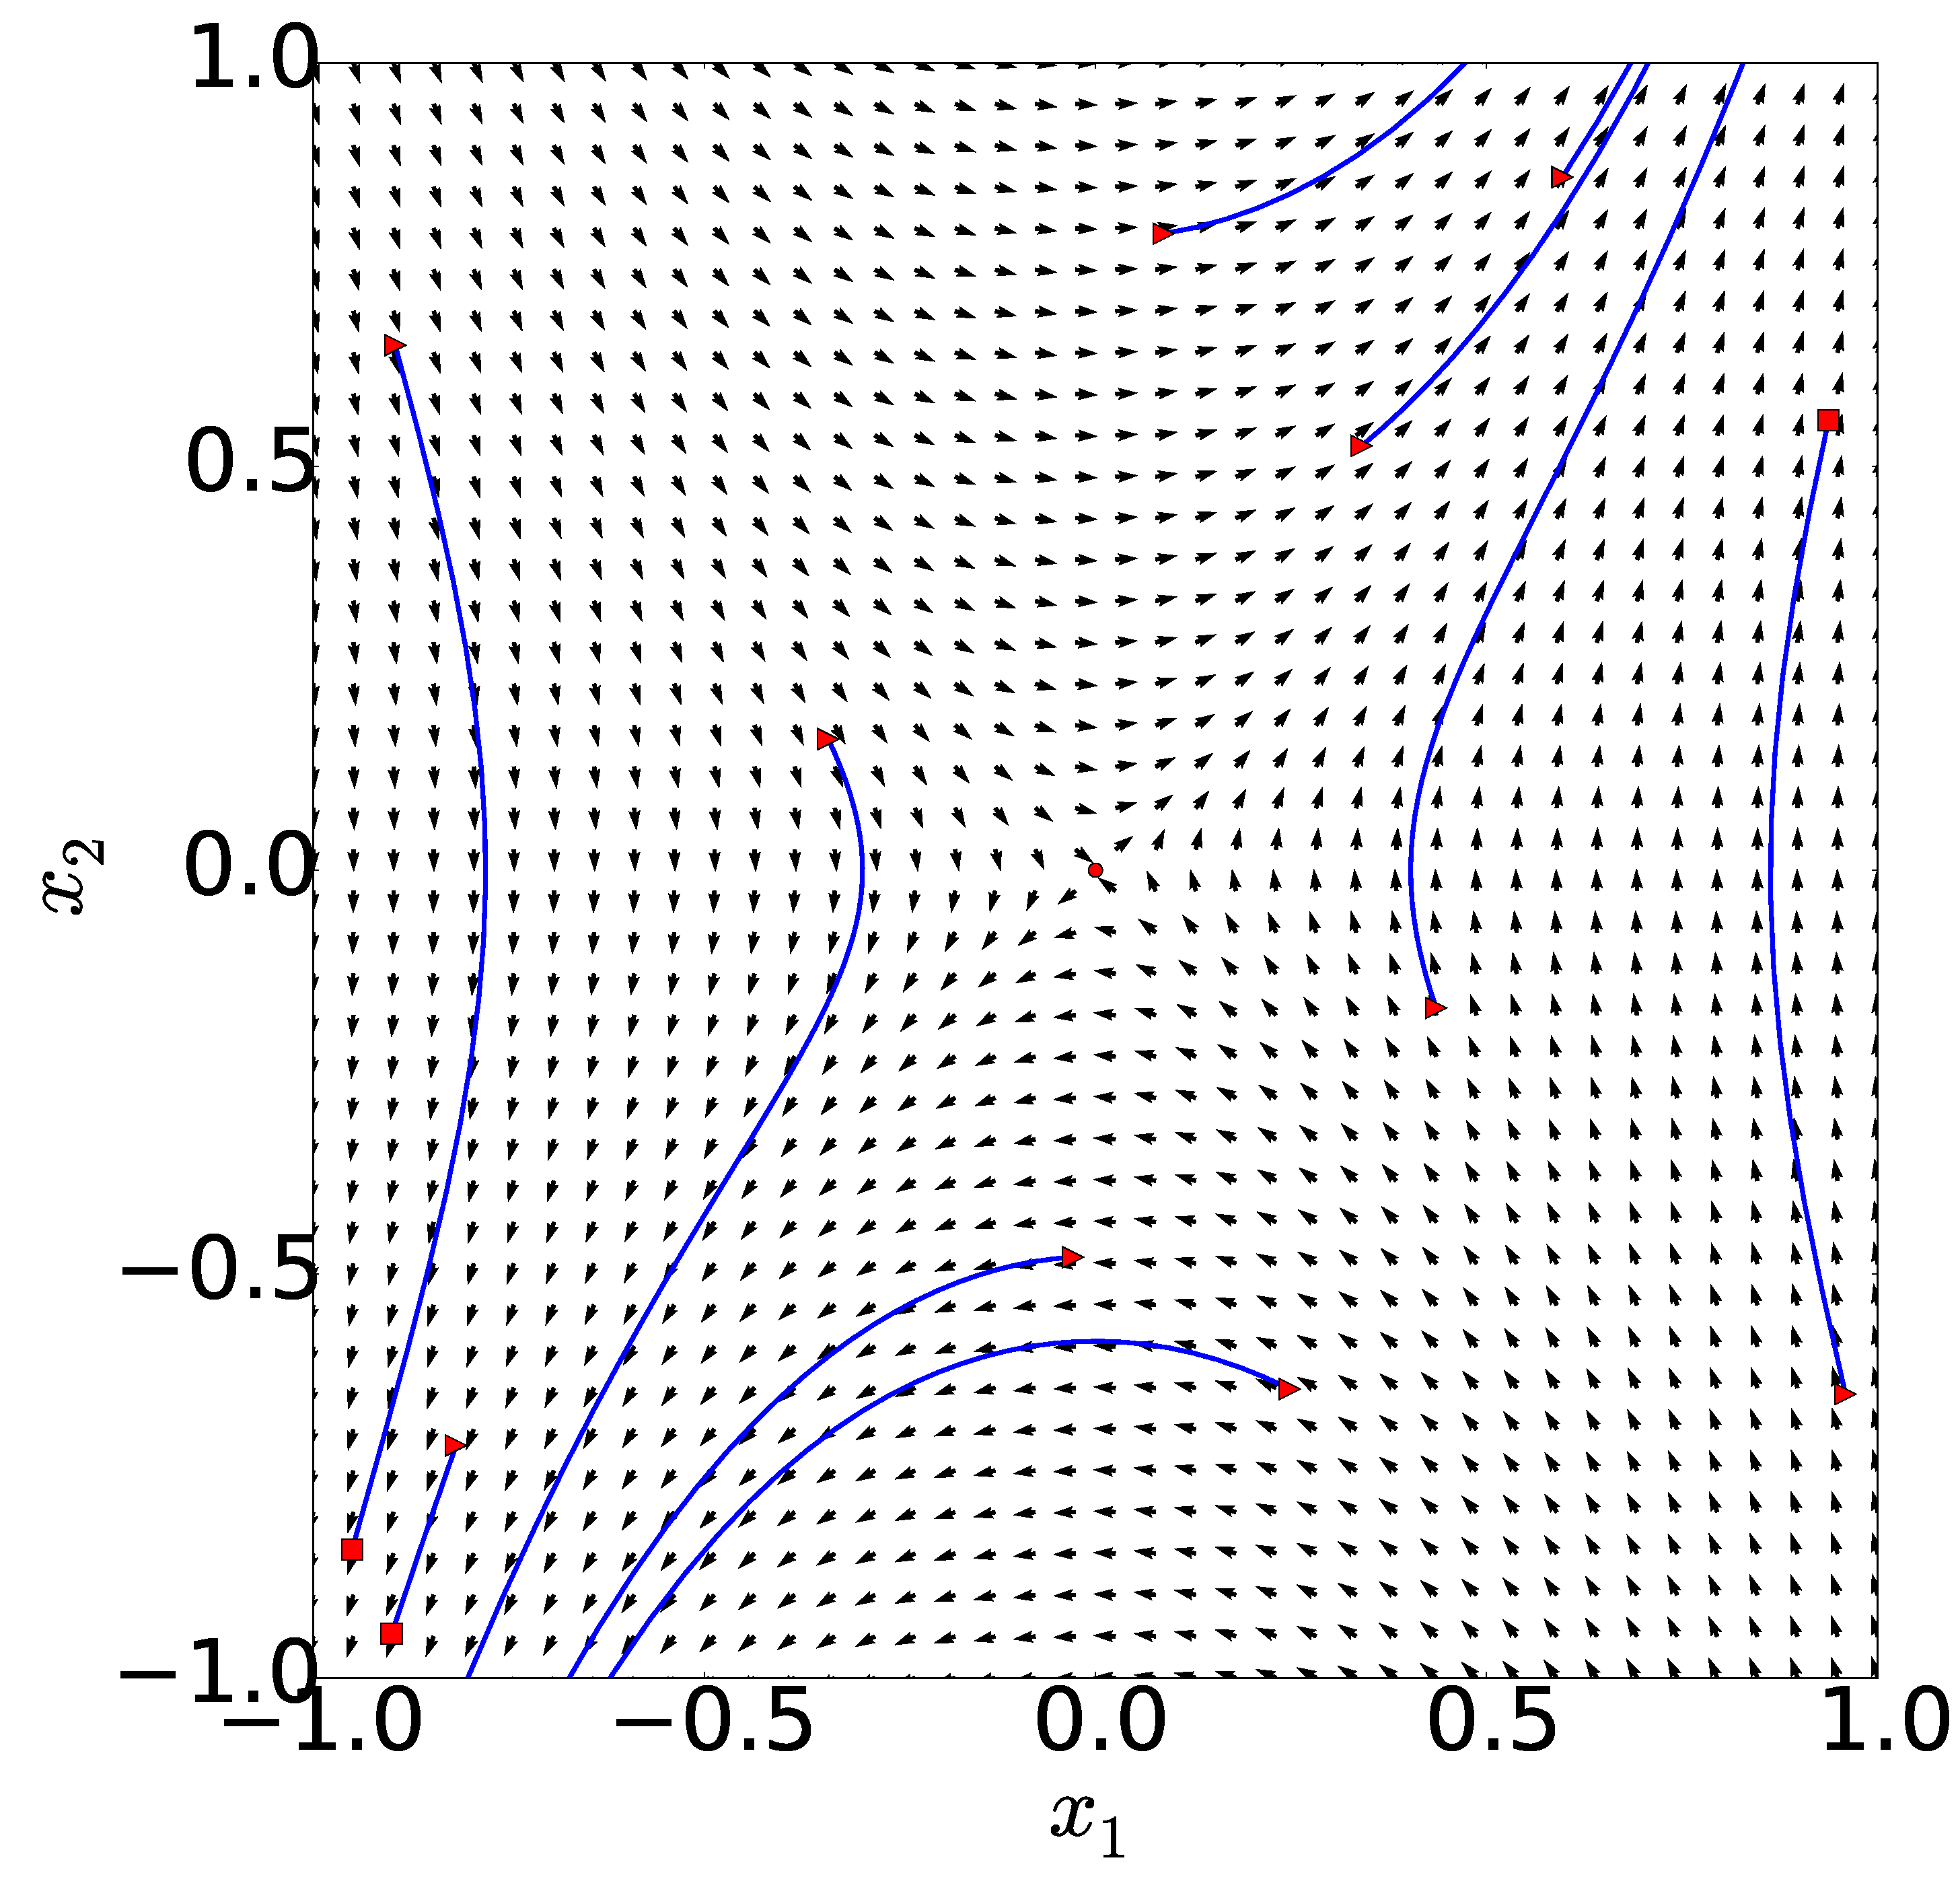
\includegraphics[width=8.0 cm]{figure/phase_portrait_around_x10_00_x20_0_3.eps}
		\caption{Case 3 - Expanded function}
    \end{subfigure}
    	\begin{subfigure}[h]{8.0 cm}
        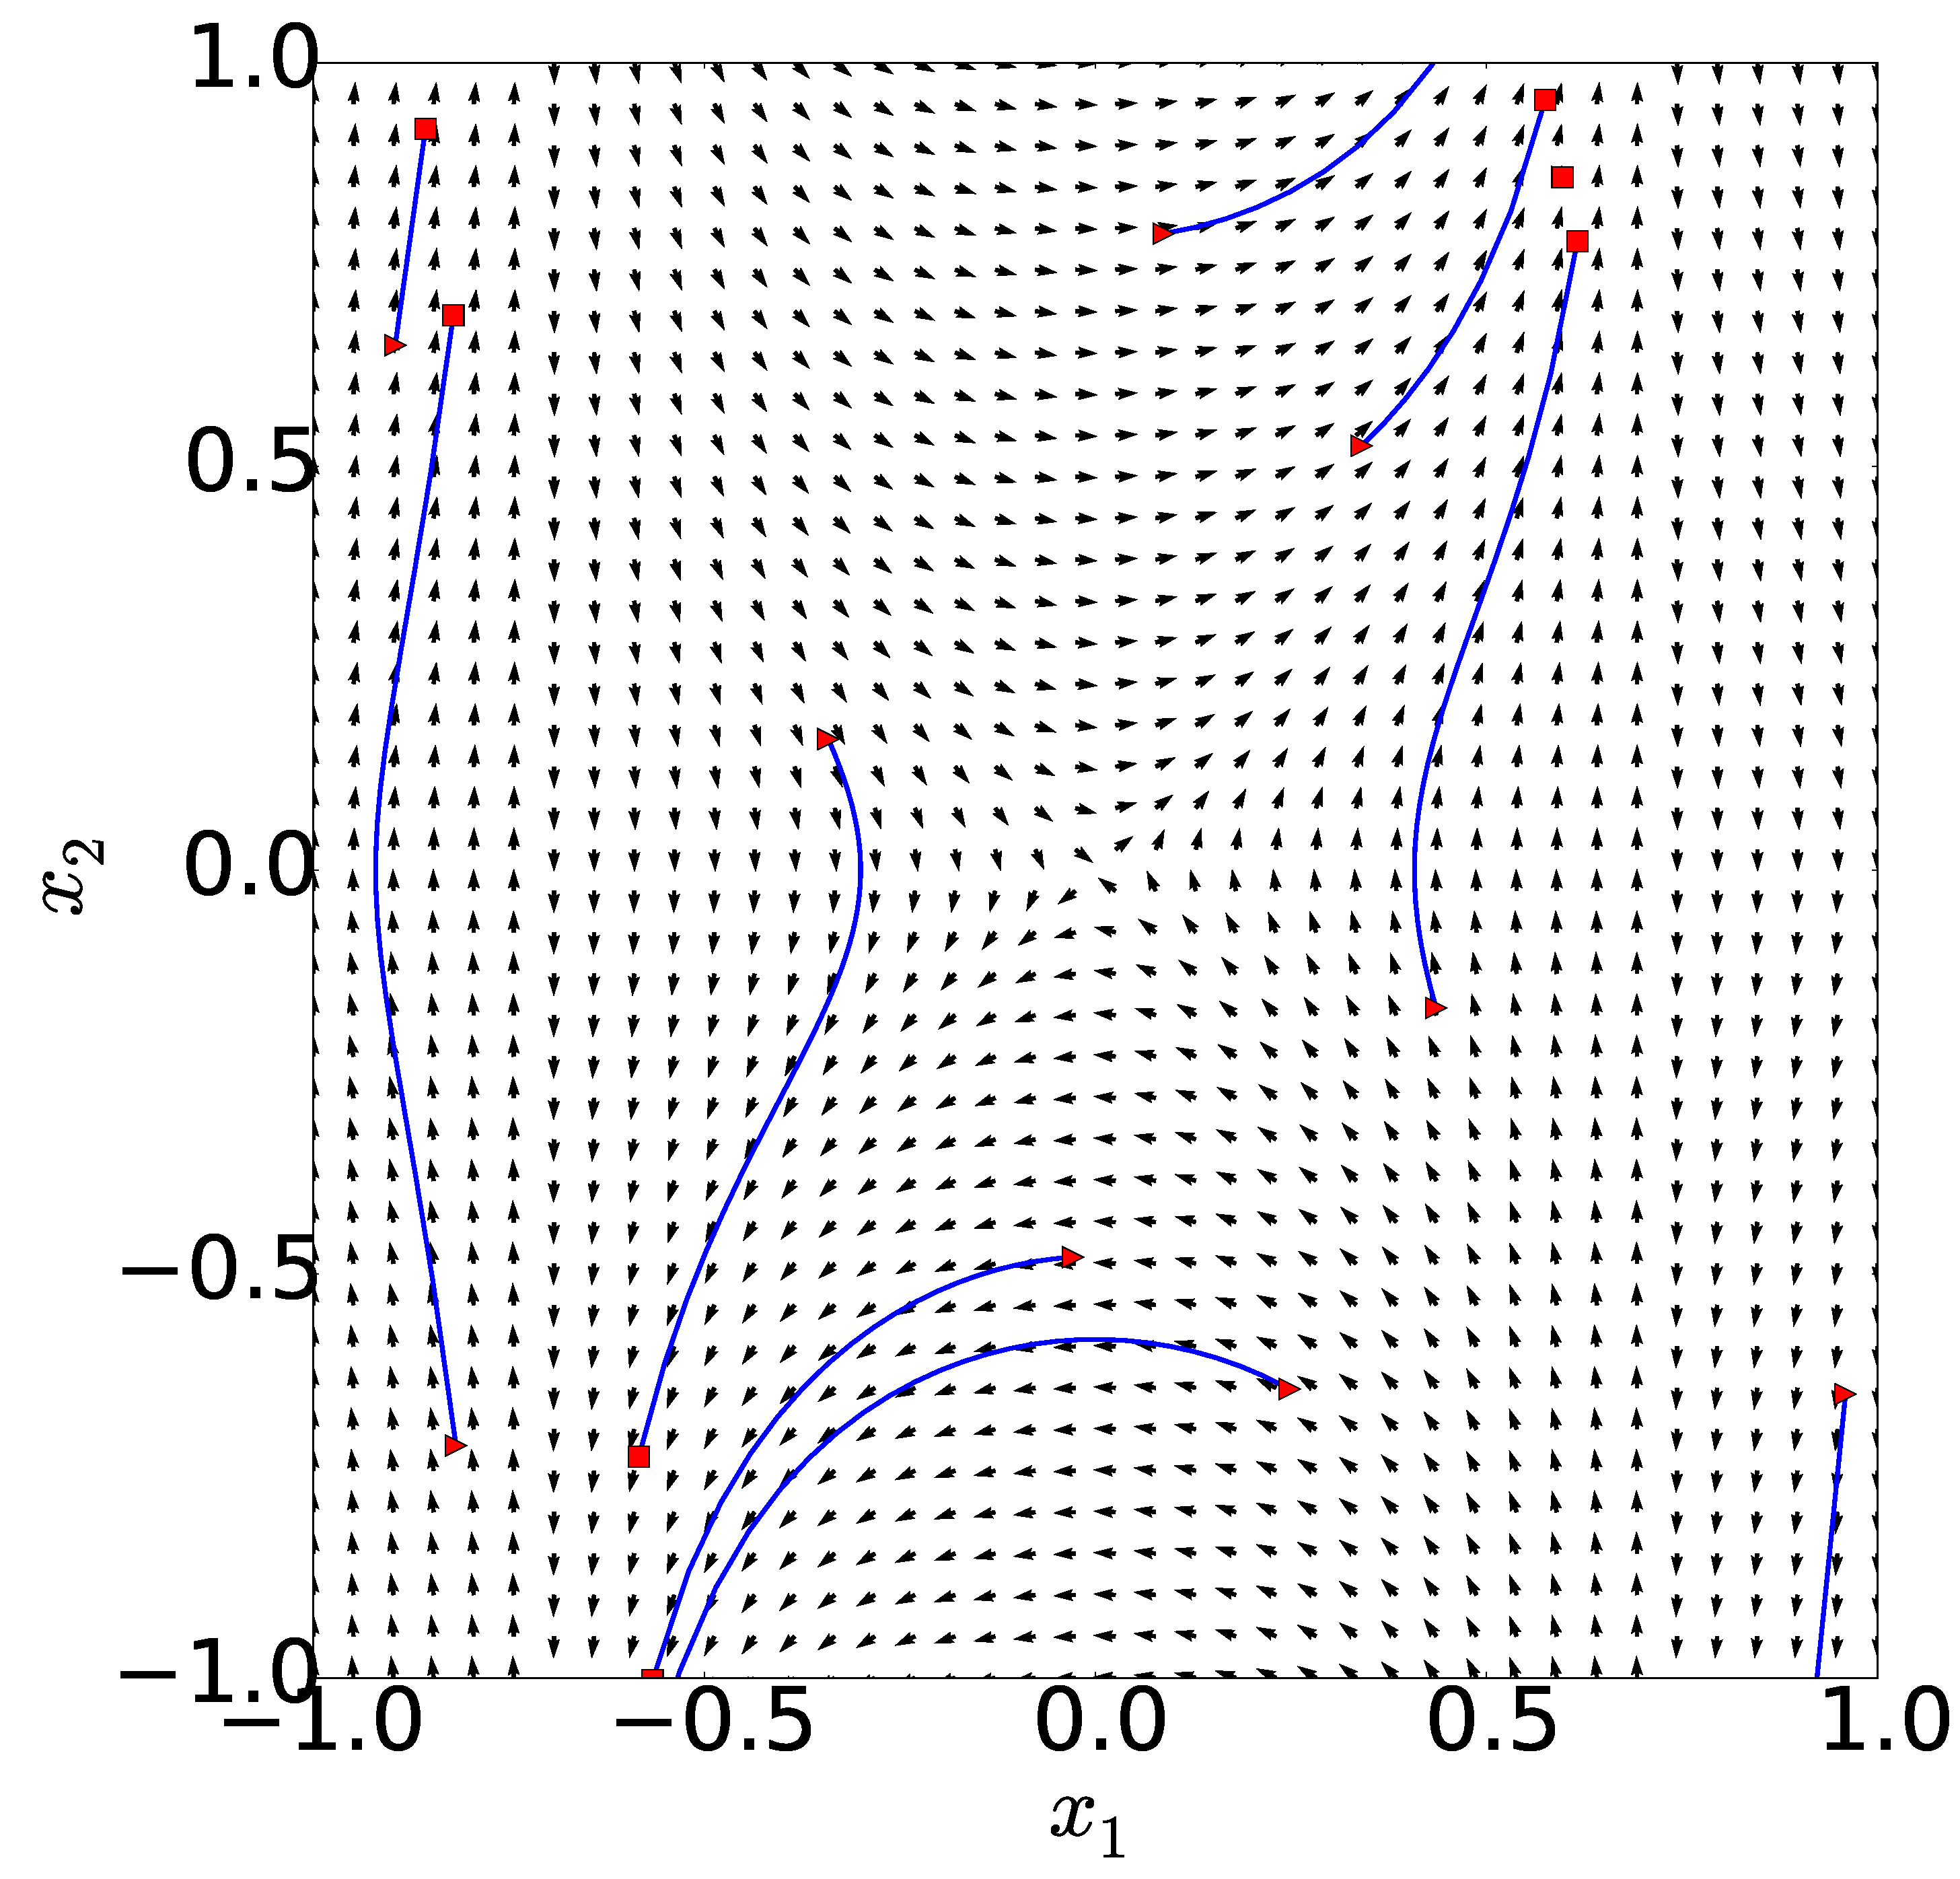
\includegraphics[width=8.0 cm]{figure/phase_portrait_l2nlcomp3.eps}
		\caption{Case 3 - Actual function}
    \end{subfigure}
    \caption{Phase plot for expanded state function around $(0, 0)$. Trajectories start from $\rhd$ and end at $\Box$. All trajectories are integrated for $10$ seconds.}
    \label{fig:PhasePlotExpanded0}
\end{figure}

The values selected in Table \ref{table:systemConstantsExpanded0} reflect the three conditions of stability. Case 1 is the stable system, case 2 is unstable, and case 3 is the central point. This is also can be seen in the phase plot of Figure \ref{fig:PhasePlotExpanded0}.\\

\textbf{Second stationary point: }$\mathbf{(x_1, x_2) = (\sqrt{1 - \left( \dfrac{m_1 \epsilon g}{kl} \right)^2}, 0)}:$

Since the symbolic notation for the fixed point will become too long, we will investigate its characteristics by substituting different values for systems constants. The constants are chosen according to Table \ref{table:systemConstantsExpanded1}. It should be noted that the constants need to satisfy Equation \eqref{eq:stationaryPointCondition} for this stationary point to exist.

\begin{table}[htbp]
\begin{center}
\begin{tabular}{c||c|c|c|c|c|c}
case number & $\epsilon$ & $k$ & $m_1$ & $g$ & $l$ & $\dfrac{m_1 \epsilon g}{k l}$ \\ \hline \hline
1 & -0.1 & 1 & 1 & 1 & 1 & -0.1 \\ \hline
2 & -2 & 4 & 1.6 & 3 & 5 & -0.48 \\ \hline
3 & -1 & 3 & 1 & 2 & 1 & -0.667 \\
\end{tabular}
\end{center}
\caption{System constants}
\label{table:systemConstantsExpanded1}
\end{table}

The phase plots are shown in Figure \ref{fig:PhasePlotExpanded1}. To better understand the characteristic of stationary points, we look at the eigenvalues of linearized state equation for each of the cases in Table \ref{table:systemConstantsExpanded1}. This is shown in Table \ref{table:Expanded1Eigenvalues1}.

\begin{table}[htbp]
\begin{center}
\begin{tabular}{c | c | c | c | c}
\multirow{2}{*}{case number} & \multicolumn{2}{| c |}{Expansion point} & \multicolumn{2}{| c}{Eigenvalues} \\ \cline{2-5}
  & $x_1$ & $x_2$ & $\lambda_1$ & $\lambda_2$ \\ \hline
1 & 0.99 & 0 & -3.33i & 3.33i \\ \hline
2 & 0.87 & 0 & -1.92i & 1.92i \\ \hline
3 & 0.74 & 0 & -3.87i & 3.87i \\
\end{tabular}
\end{center}
\caption{System constants}
\label{table:Expanded1Eigenvalues1}
\end{table}

As can be seen here, all the eigenvectors are purely imaginary. Therefore, we cannot talk about the stability of the nonlinear system based on the linearized form of the equations. However, by looking at the phase plots of the nonlinear system, we can say that this stationary point can become stable or unstable based on the parameters that we choose for the system.

We compare the phase portrait of expanded function around the stationary point with the full function in Figure \ref{fig:PhasePlotExpanded1}. The expansion point is shown by a red circle on the figure. As Expected, the expanded function only matches the real function near the expansion point.

\begin{figure}[H]
	\centering
	\begin{subfigure}[h]{8.0 cm}
		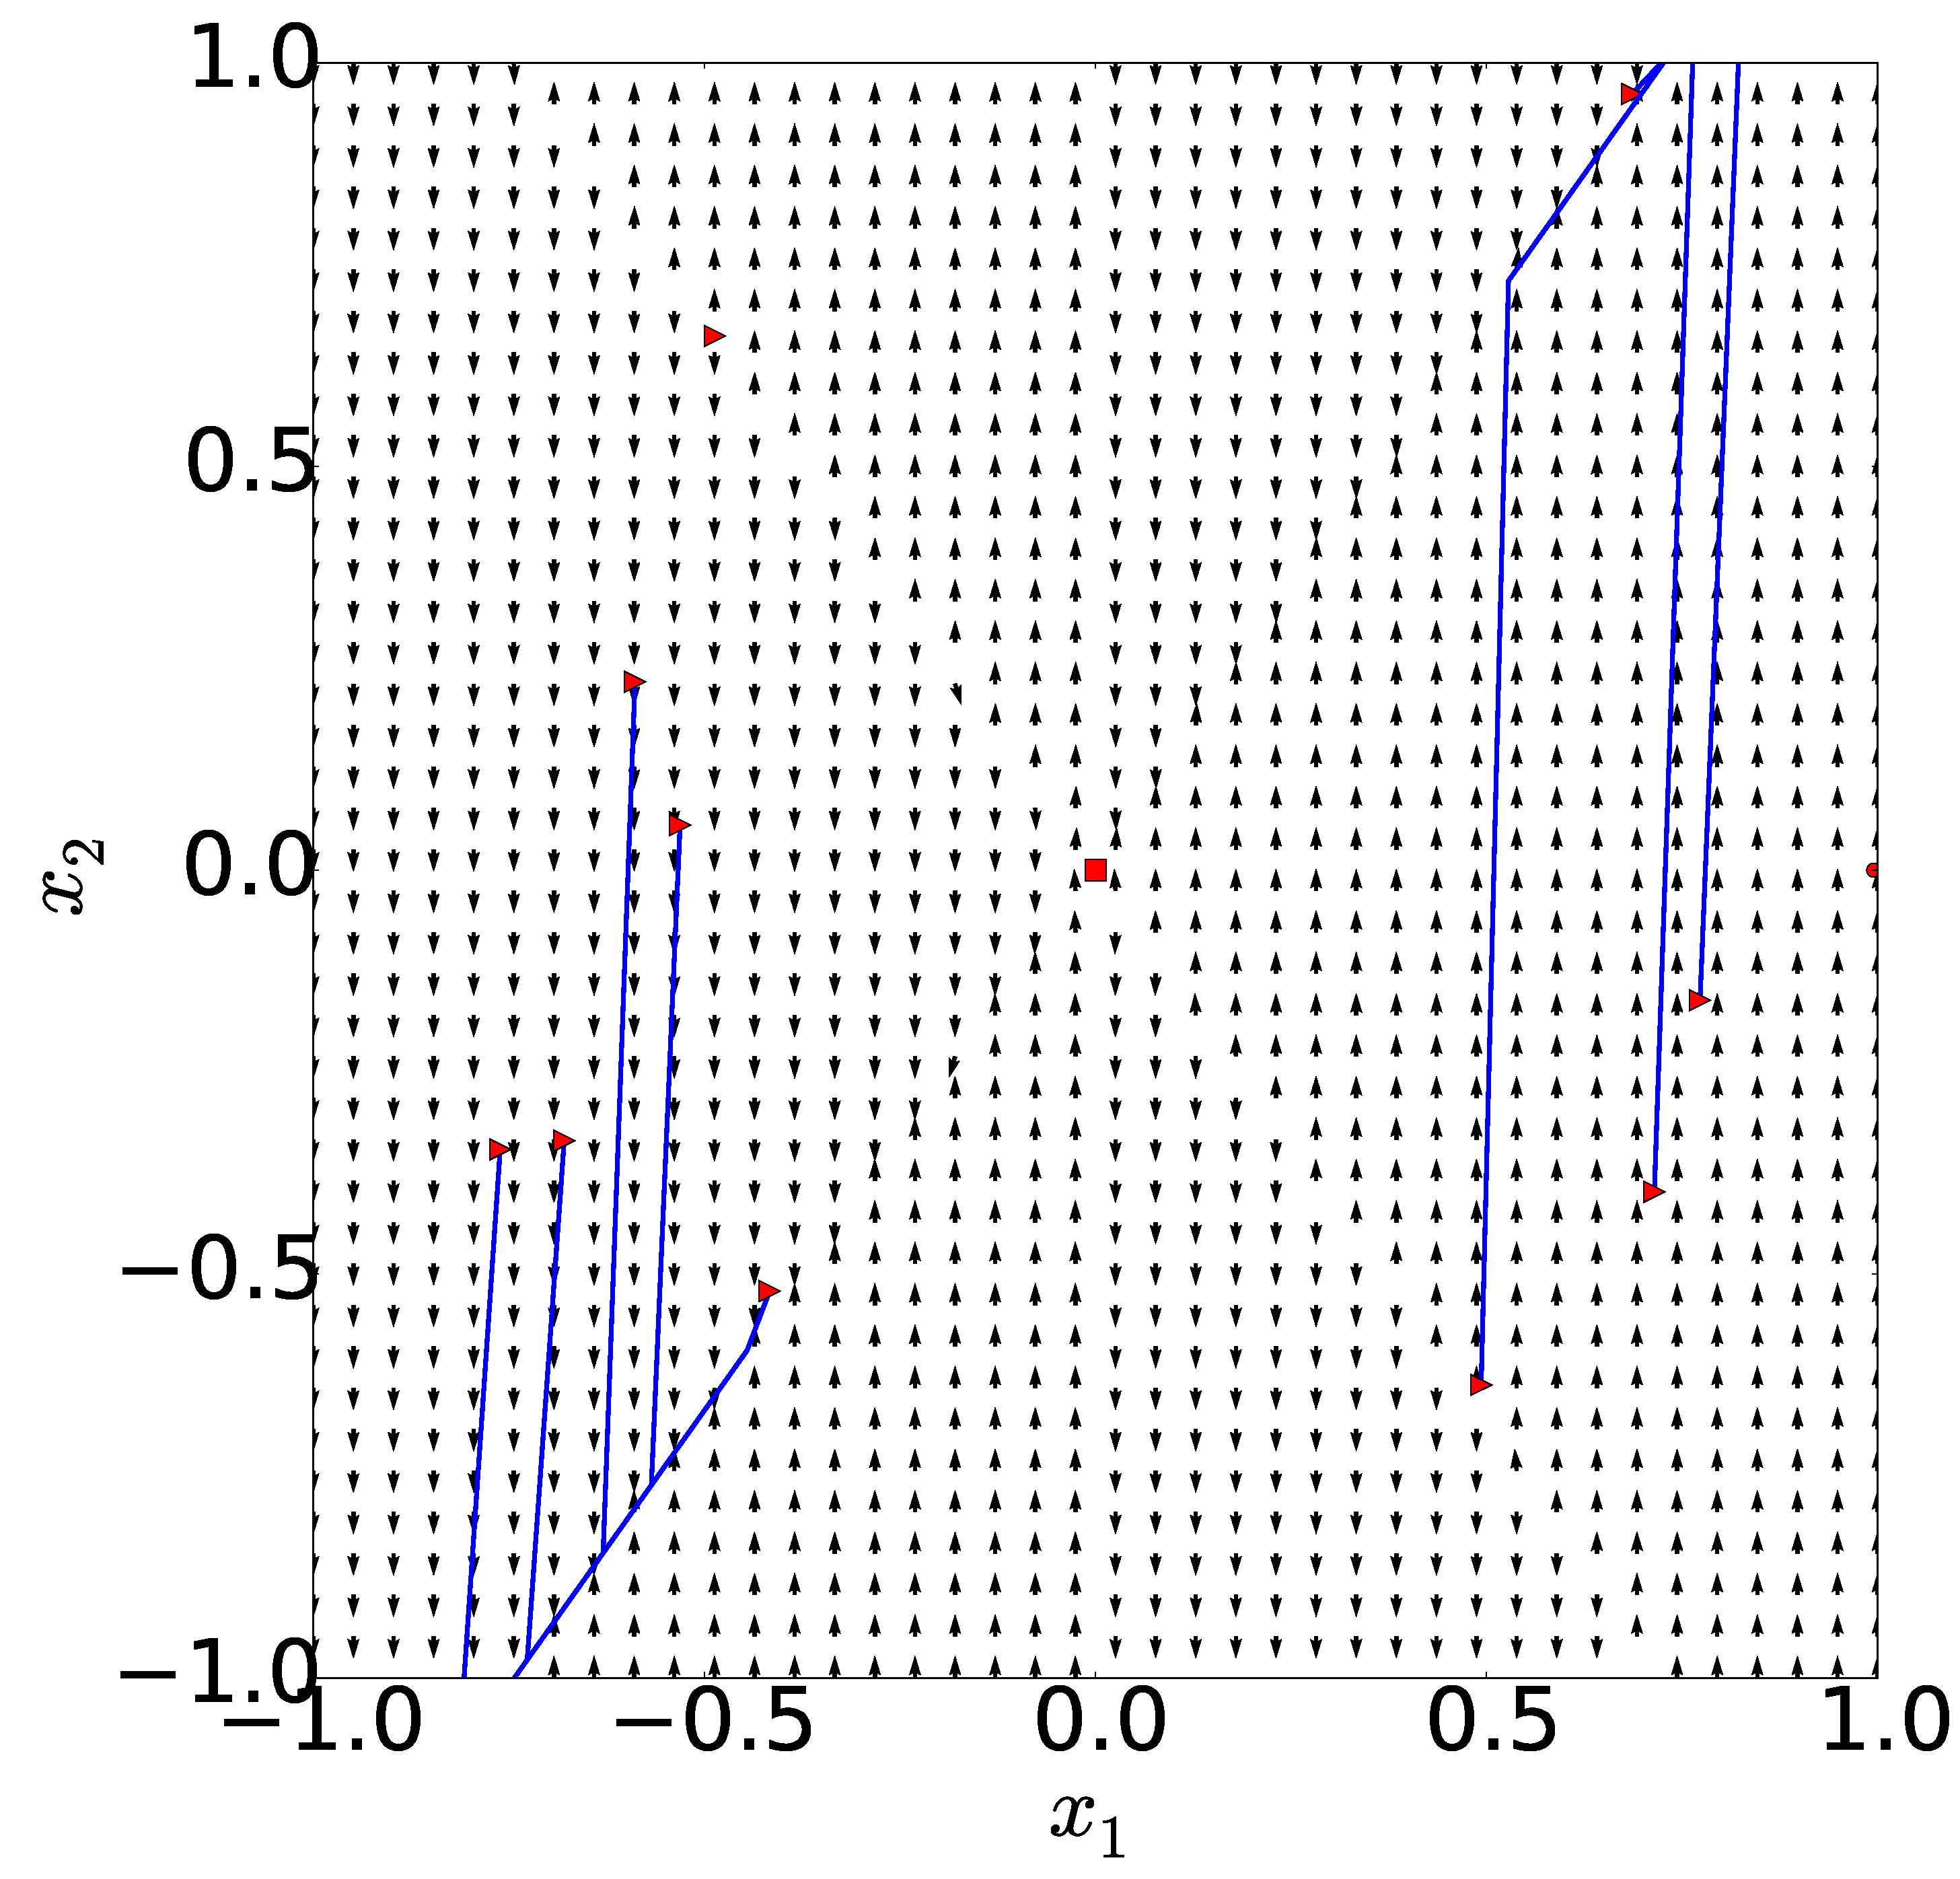
\includegraphics[width=8.0 cm]{figure/phase_portrait_around_x10_99_x20_99_1.eps}
		\caption{Case 1 - Expanded function}
	\end{subfigure}
	\begin{subfigure}[h]{8.0 cm}
        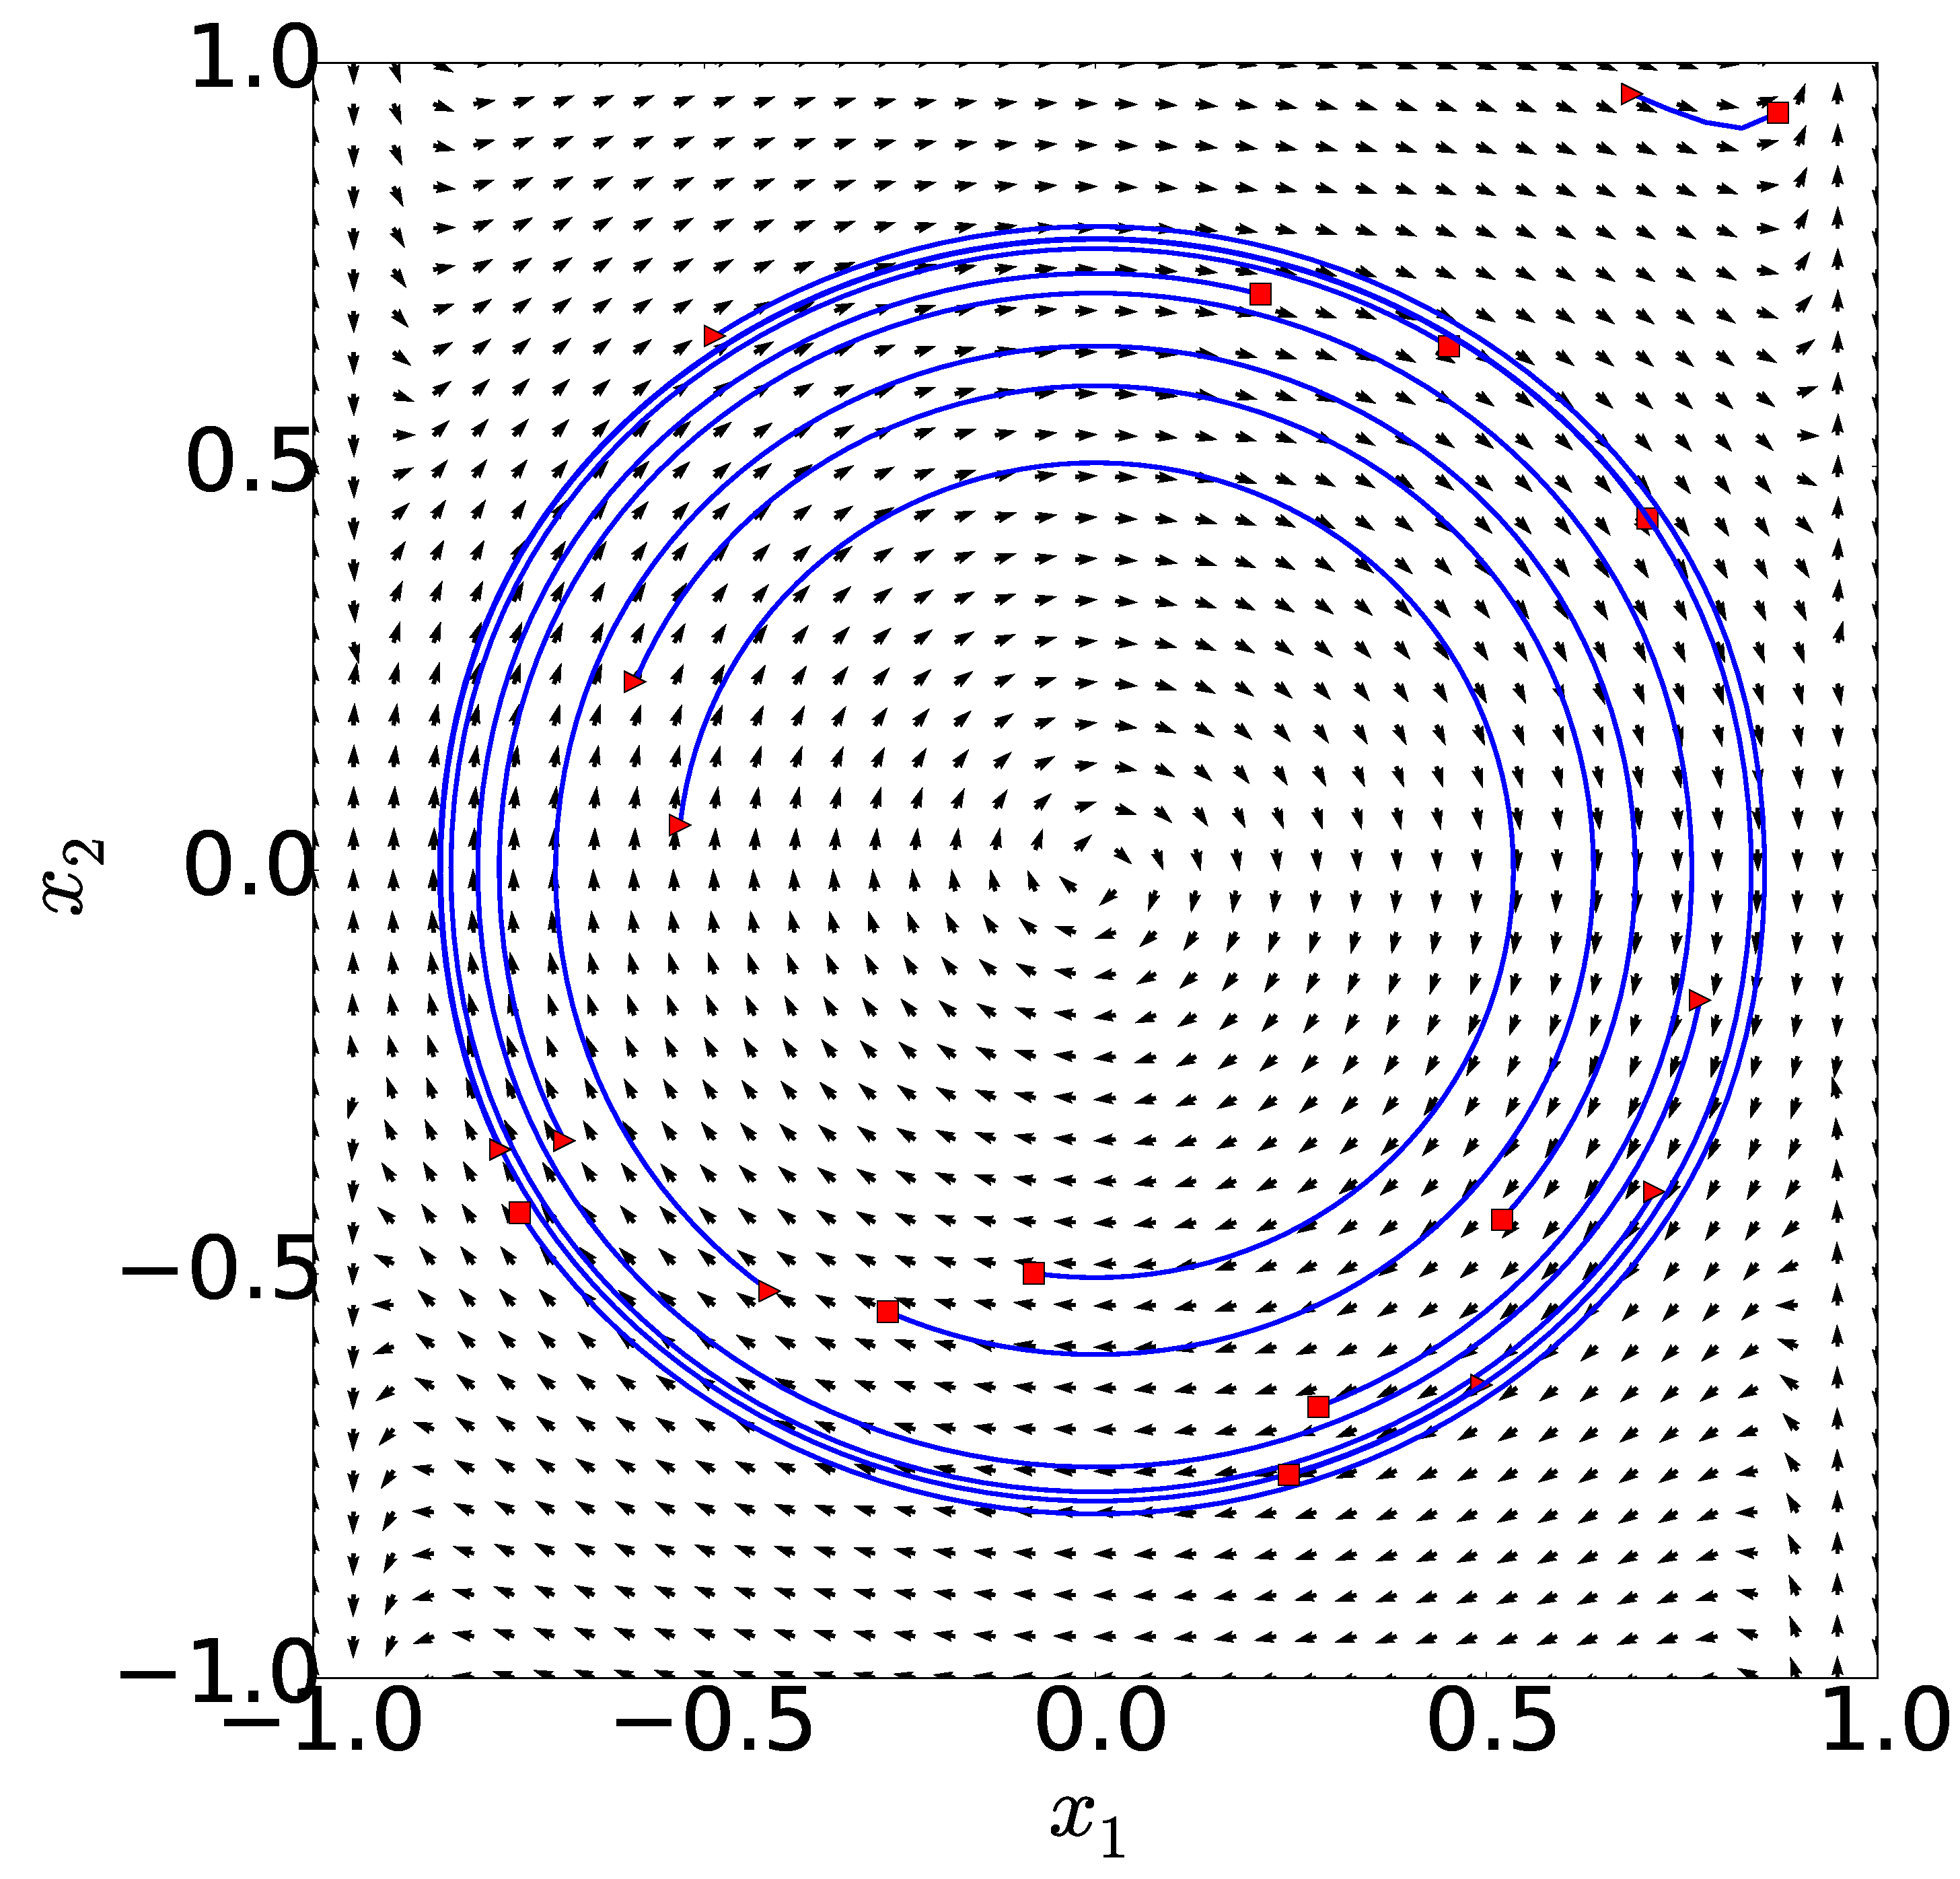
\includegraphics[width=8.0 cm]{figure/phase_portrait_l2nlcomp1_1.eps}
		\caption{Case 1 - Actual function}
    \end{subfigure}
    \\
    \begin{subfigure}[h]{8.0 cm}
		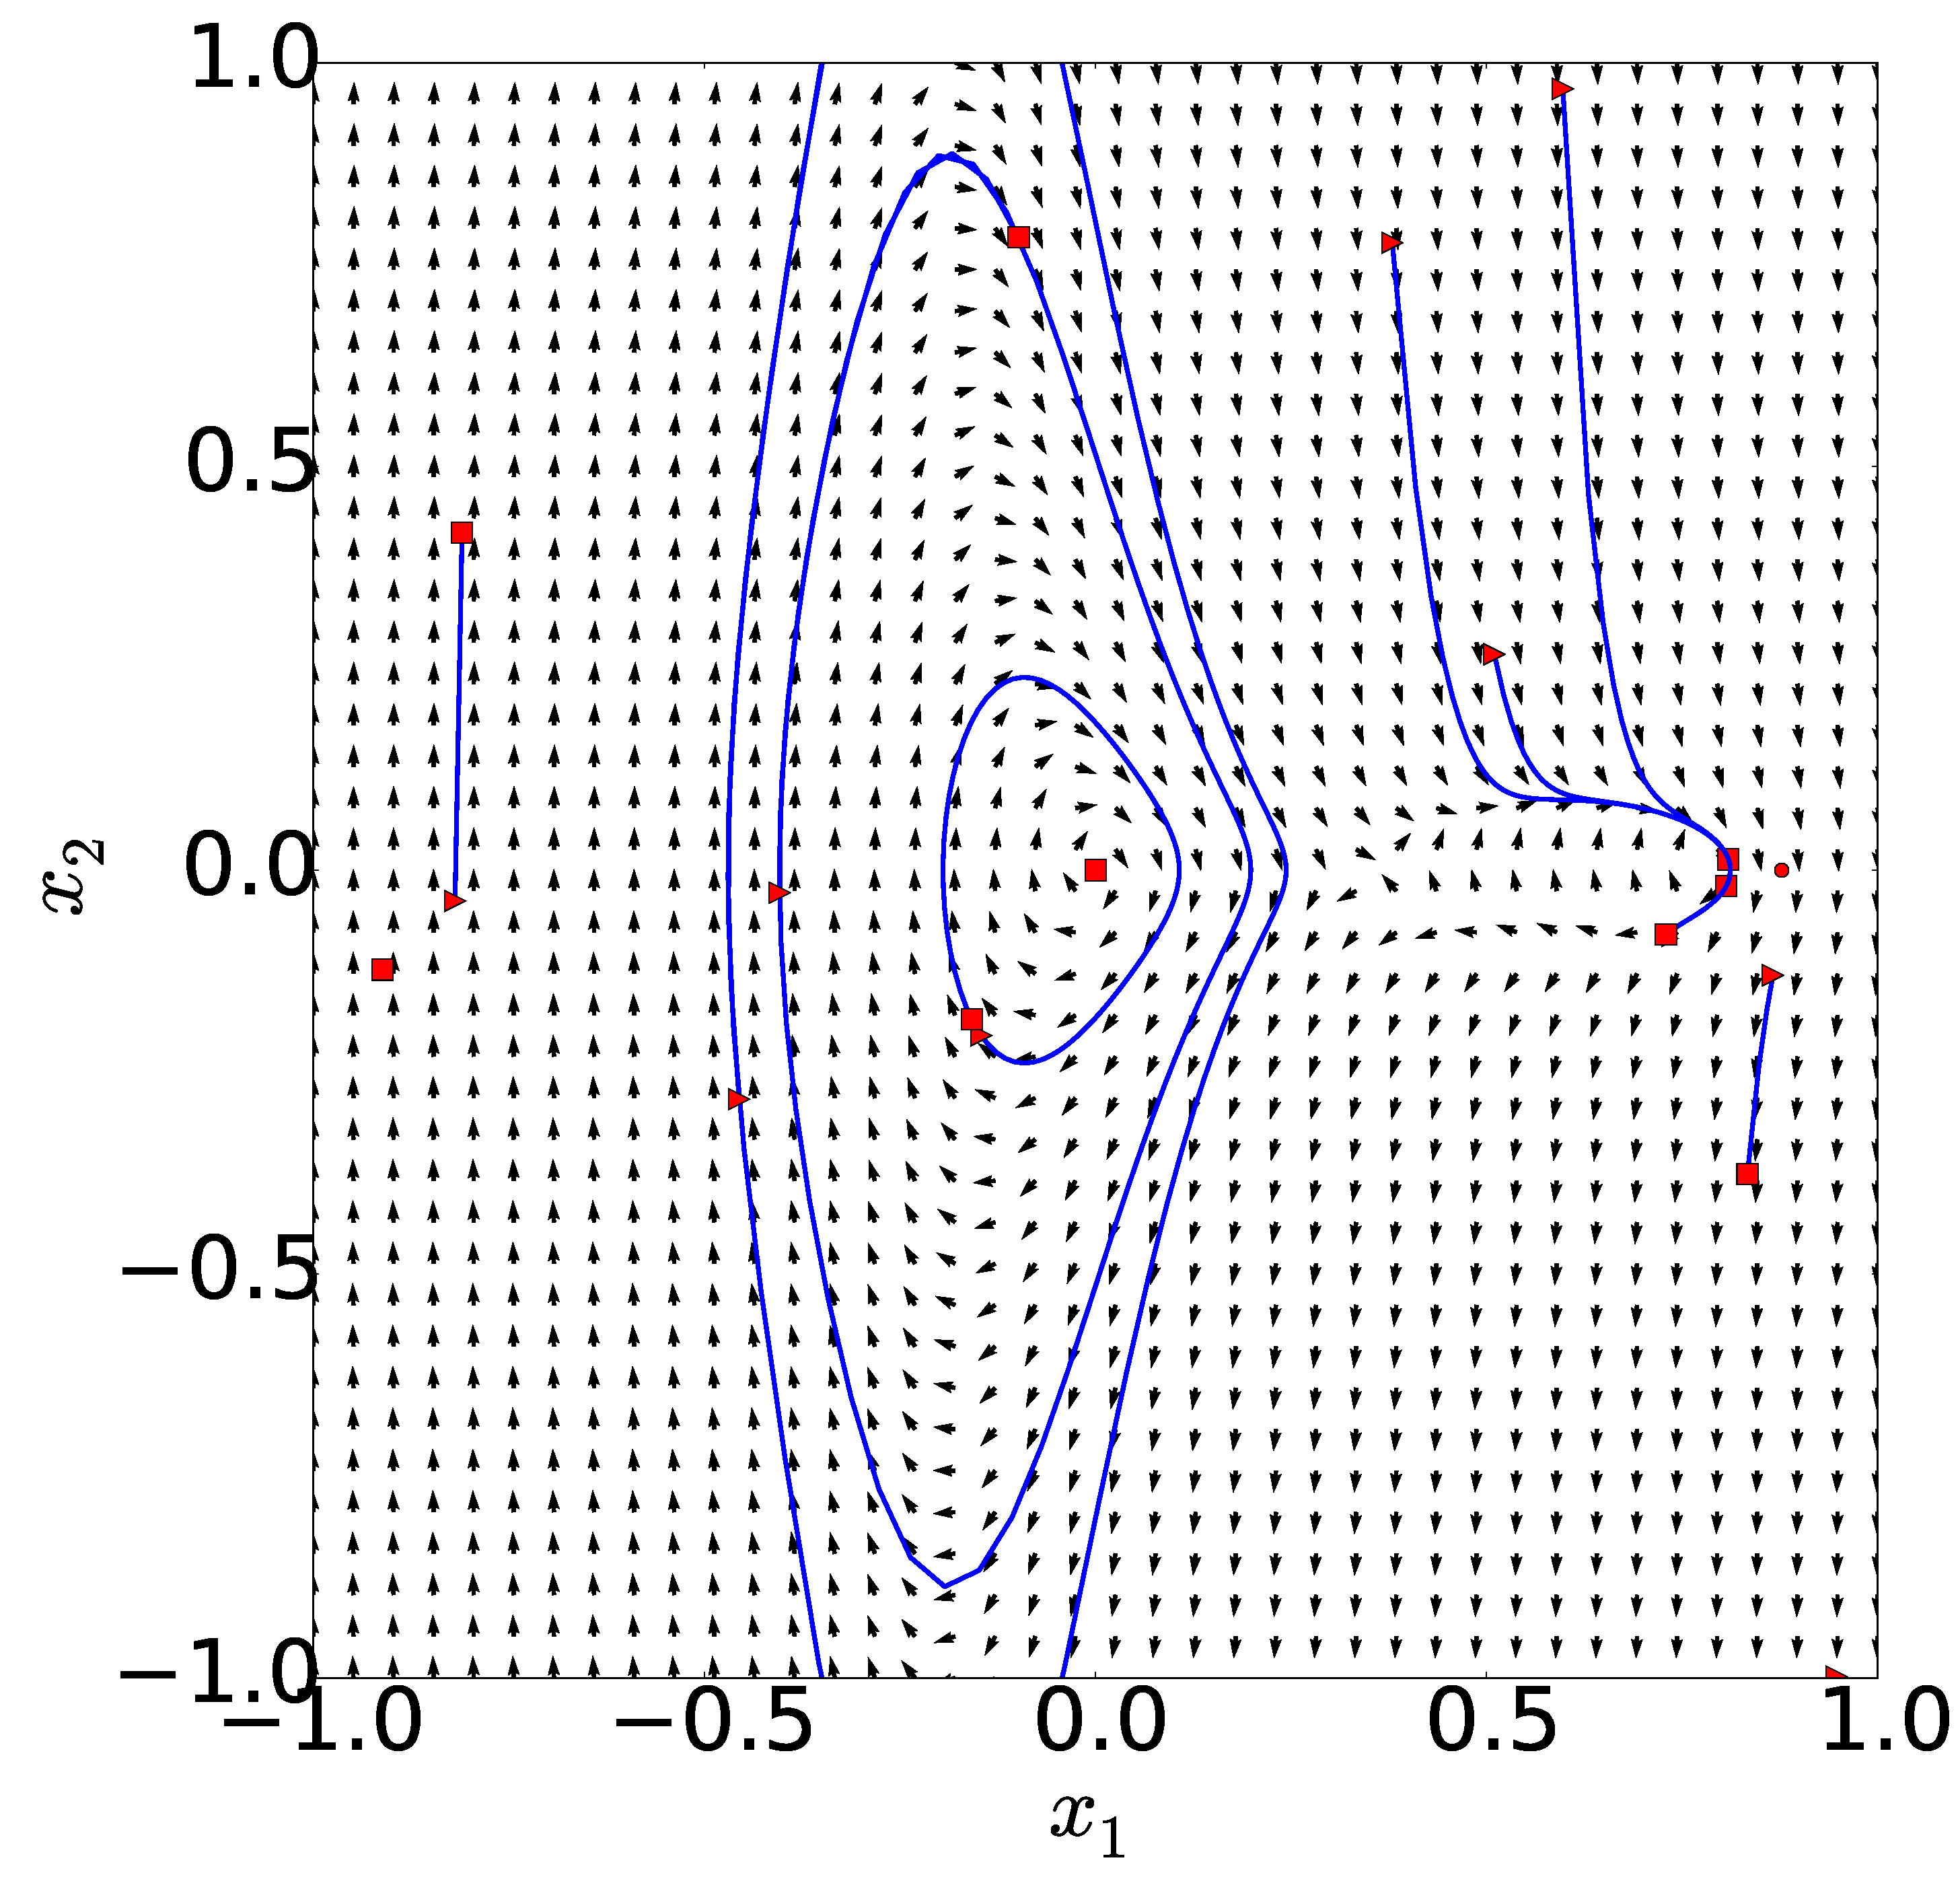
\includegraphics[width=8.0 cm]{figure/phase_portrait_around_x10_87_x20_87_2.eps}
		\caption{Case 2 - Expanded function}
	\end{subfigure}
	\begin{subfigure}[h]{8.0 cm}
        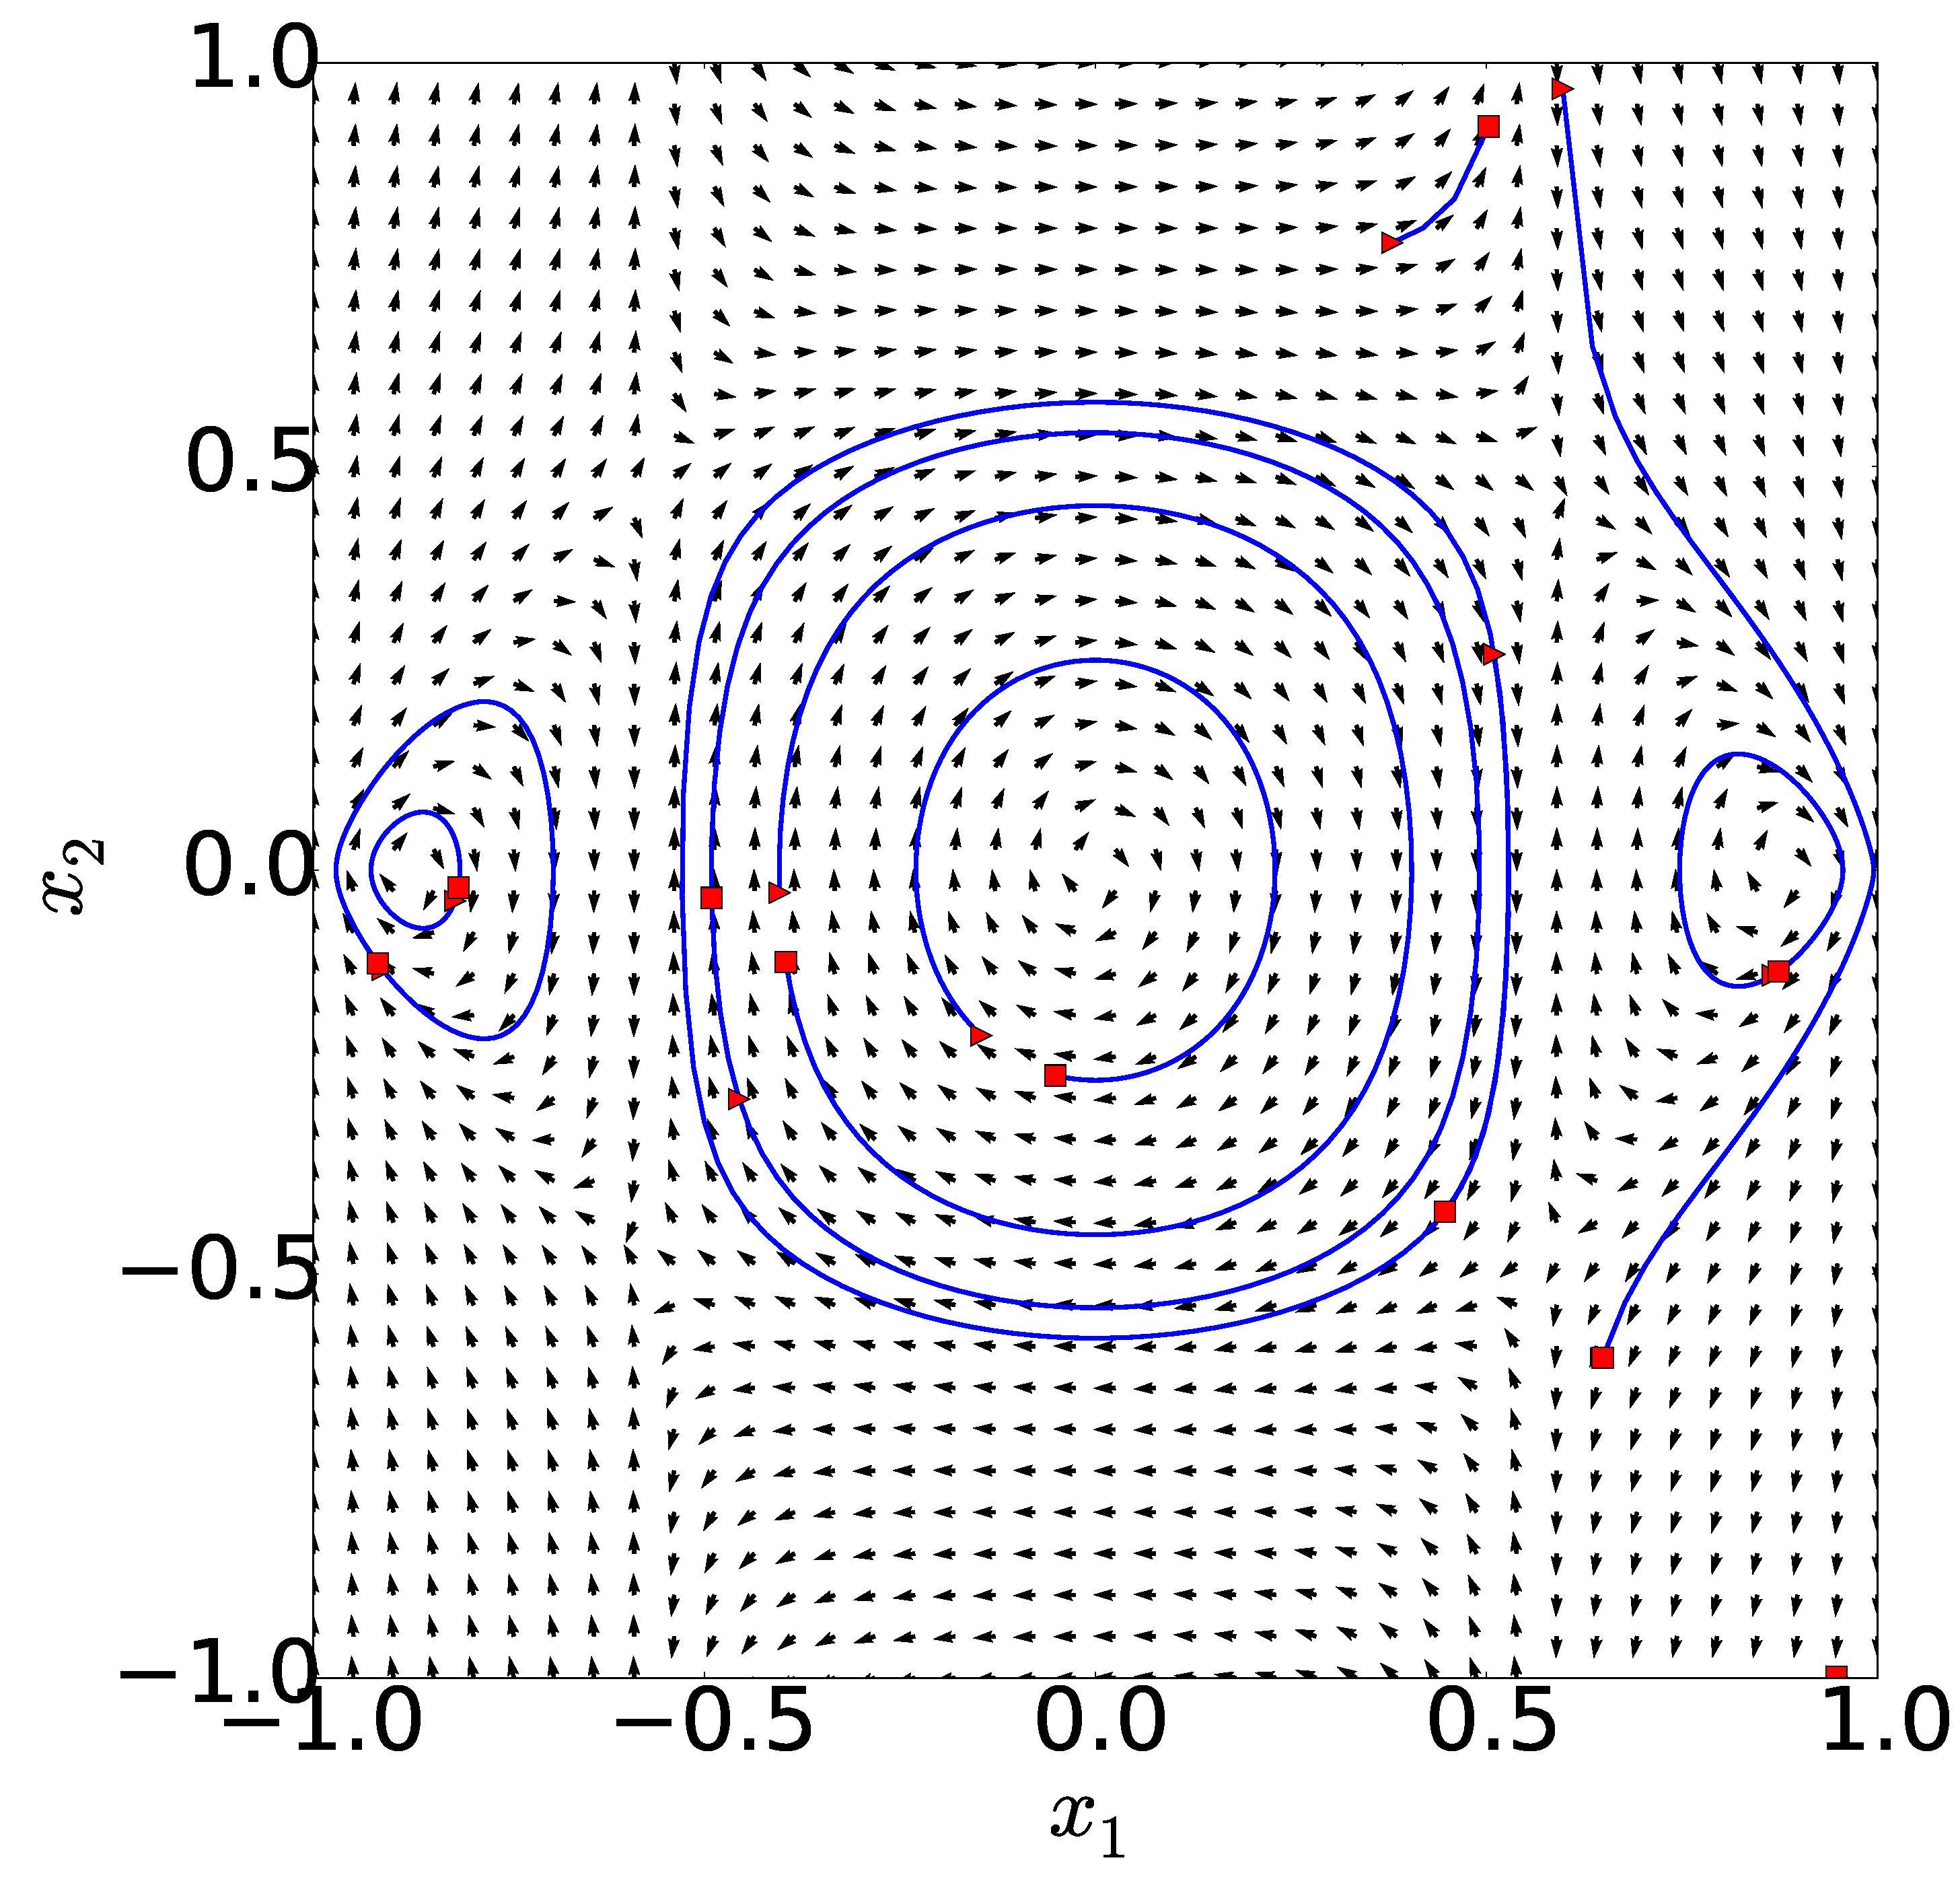
\includegraphics[width=8.0 cm]{figure/phase_portrait_l2nlcomp2_1.eps}
		\caption{Case 2 - Actual function}
    \end{subfigure}
    \\
    	\begin{subfigure}[h]{8.0 cm}
        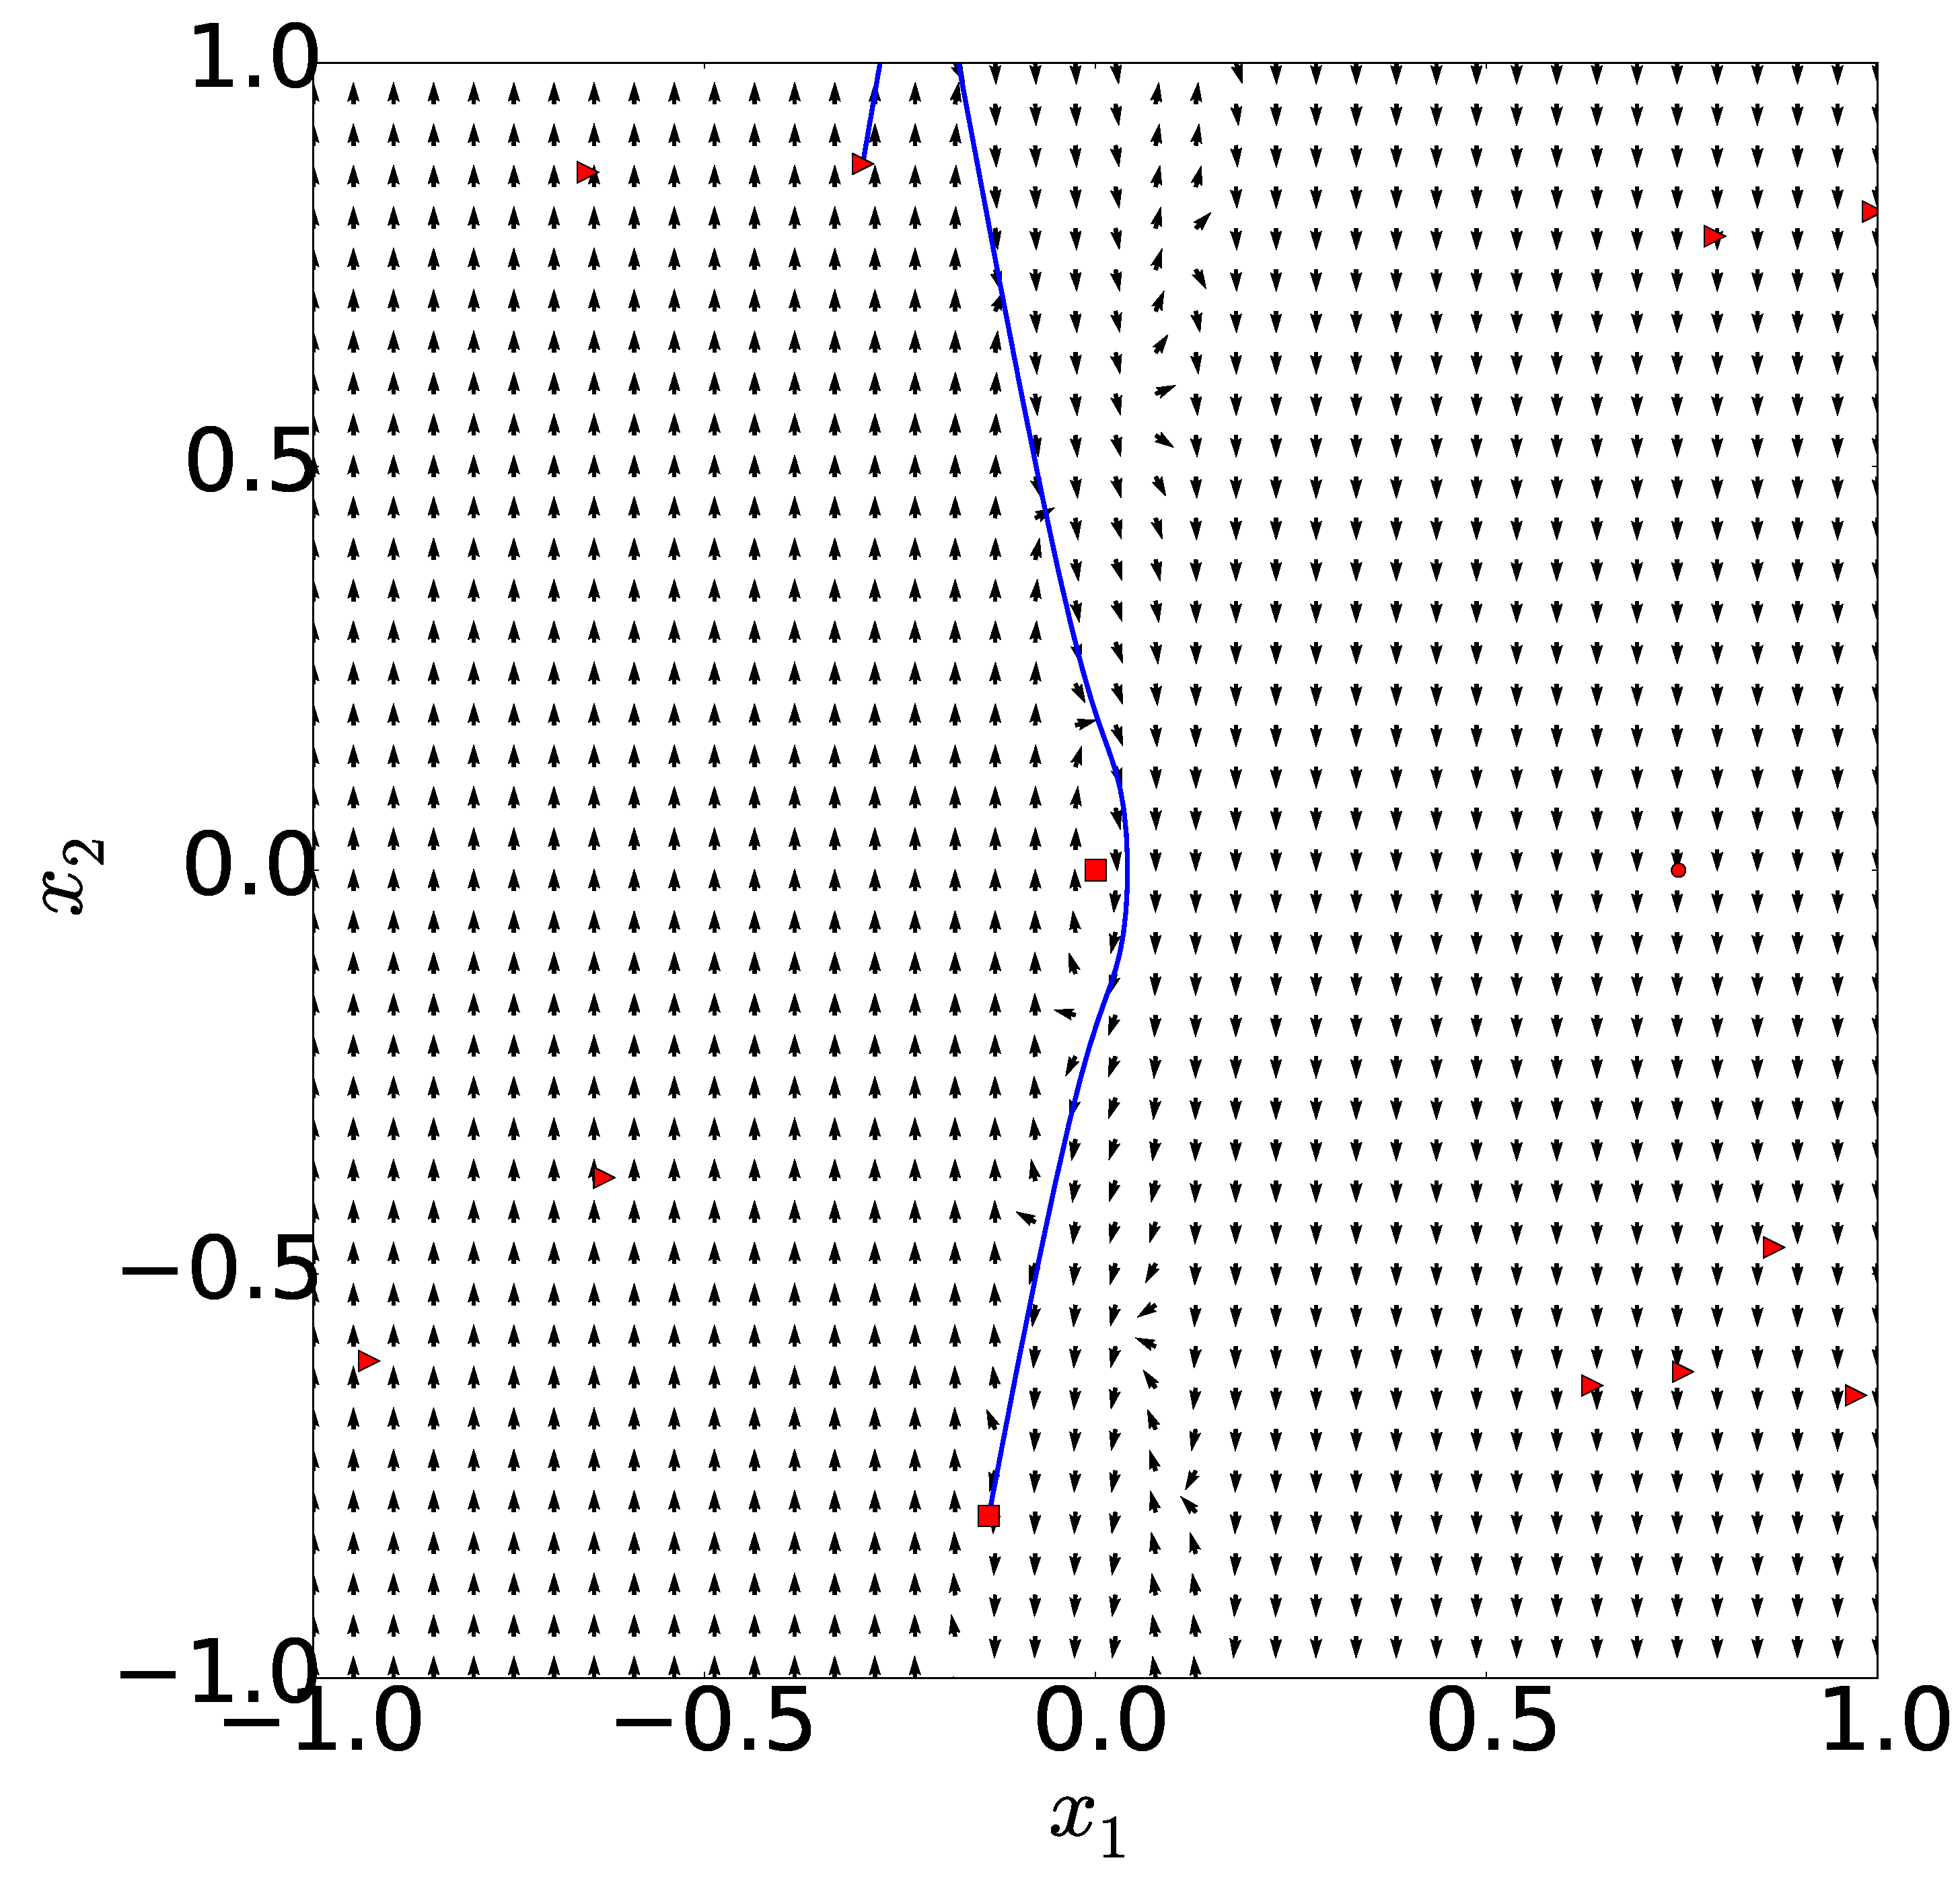
\includegraphics[width=8.0 cm]{figure/phase_portrait_around_x10_74_x20_74_3.eps}
		\caption{Case 3 - Expanded function}
    \end{subfigure}
    	\begin{subfigure}[h]{8.0 cm}
        \includegraphics[width=8.0 cm]{figure/phase_portrait_l2nlcomp3_1.eps}
		\caption{Case 3 - Actual function}
    \end{subfigure}
    \caption{Phase plot for expanded state function around $(\sqrt{1 - \left( \dfrac{m_1 \epsilon g}{kl} \right)^2}, 0)$. Trajectories start from $\rhd$ and end at $\Box$. All trajectories are integrated for $10$ seconds.}
    \label{fig:PhasePlotExpanded1}
\end{figure}

\textbf{Third stationary point: }$\mathbf{(x_1, x_2) = (-\sqrt{1 - \left( \dfrac{m_1 \epsilon g}{kl} \right)^2}, 0)}:$

For this point we need to satisfy the constants of Equation \eqref{eq:stationaryPointCondition}. Therefore, we will chose our system constants as shown in Table \ref{table:systemConstantsExpanded2}.

\begin{table}[htbp]
\begin{center}
\begin{tabular}{c||c|c|c|c|c|c}
case number & $\epsilon$ & $k$ & $m_1$ & $g$ & $l$ & $\dfrac{m_1 \epsilon g}{k l}$ \\ \hline \hline
1 & -0.1 & 1 & 1 & 1 & 1 & -0.1 \\ \hline
2 & -2 & 4 & 1.6 & 3 & 5 & -0.48 \\ \hline
3 & -1 & 3 & 1 & 2 & 1 & -0.667 \\
\end{tabular}
\end{center}
\caption{System constants}
\label{table:systemConstantsExpanded2}
\end{table}

The phase plots are shown in Figure \ref{fig:PhasePlotExpanded1}. To better understand the characteristic of stationary points, we look at the eigenvalues of linearized state equation for each of the cases in Table \ref{table:systemConstantsExpanded2}. This is shown in Table \ref{table:Expanded1Eigenvalues2}.

\begin{table}[htbp]
\begin{center}
\begin{tabular}{c | c | c | c | c}
\multirow{2}{*}{case number} & \multicolumn{2}{| c |}{Expansion point} & \multicolumn{2}{| c}{Eigenvalues} \\ \cline{2-5}
  & $x_1$ & $x_2$ & $\lambda_1$ & $\lambda_2$ \\ \hline
1 & -0.99 & 0 & -3.33i & 3.33i \\ \hline
2 & -0.87 & 0 & -1.92i & 1.92i \\ \hline
3 & -0.74 & 0 & -3.87i & 3.87i \\
\end{tabular}
\end{center}
\caption{System constants}
\label{table:Expanded1Eigenvalues2}
\end{table}

As can be seen here, all the eigenvectors are purely imaginary. Therefore, we cannot talk about the stability of the nonlinear system based on the linearized form of the equations. However, by looking at the phase plots of the nonlinear system, we can say that this stationary point can become stable or unstable based on the parameters that we choose for the system.

We compare the phase portrait of expanded function around the stationary point with the full function in Figure \ref{fig:PhasePlotExpanded2}. The expansion point is shown by a red circle on the figure. As Expected, the expanded function only matches the real function near the expansion point.

\begin{figure}[H]
	\centering
	\begin{subfigure}[h]{8.0 cm}
		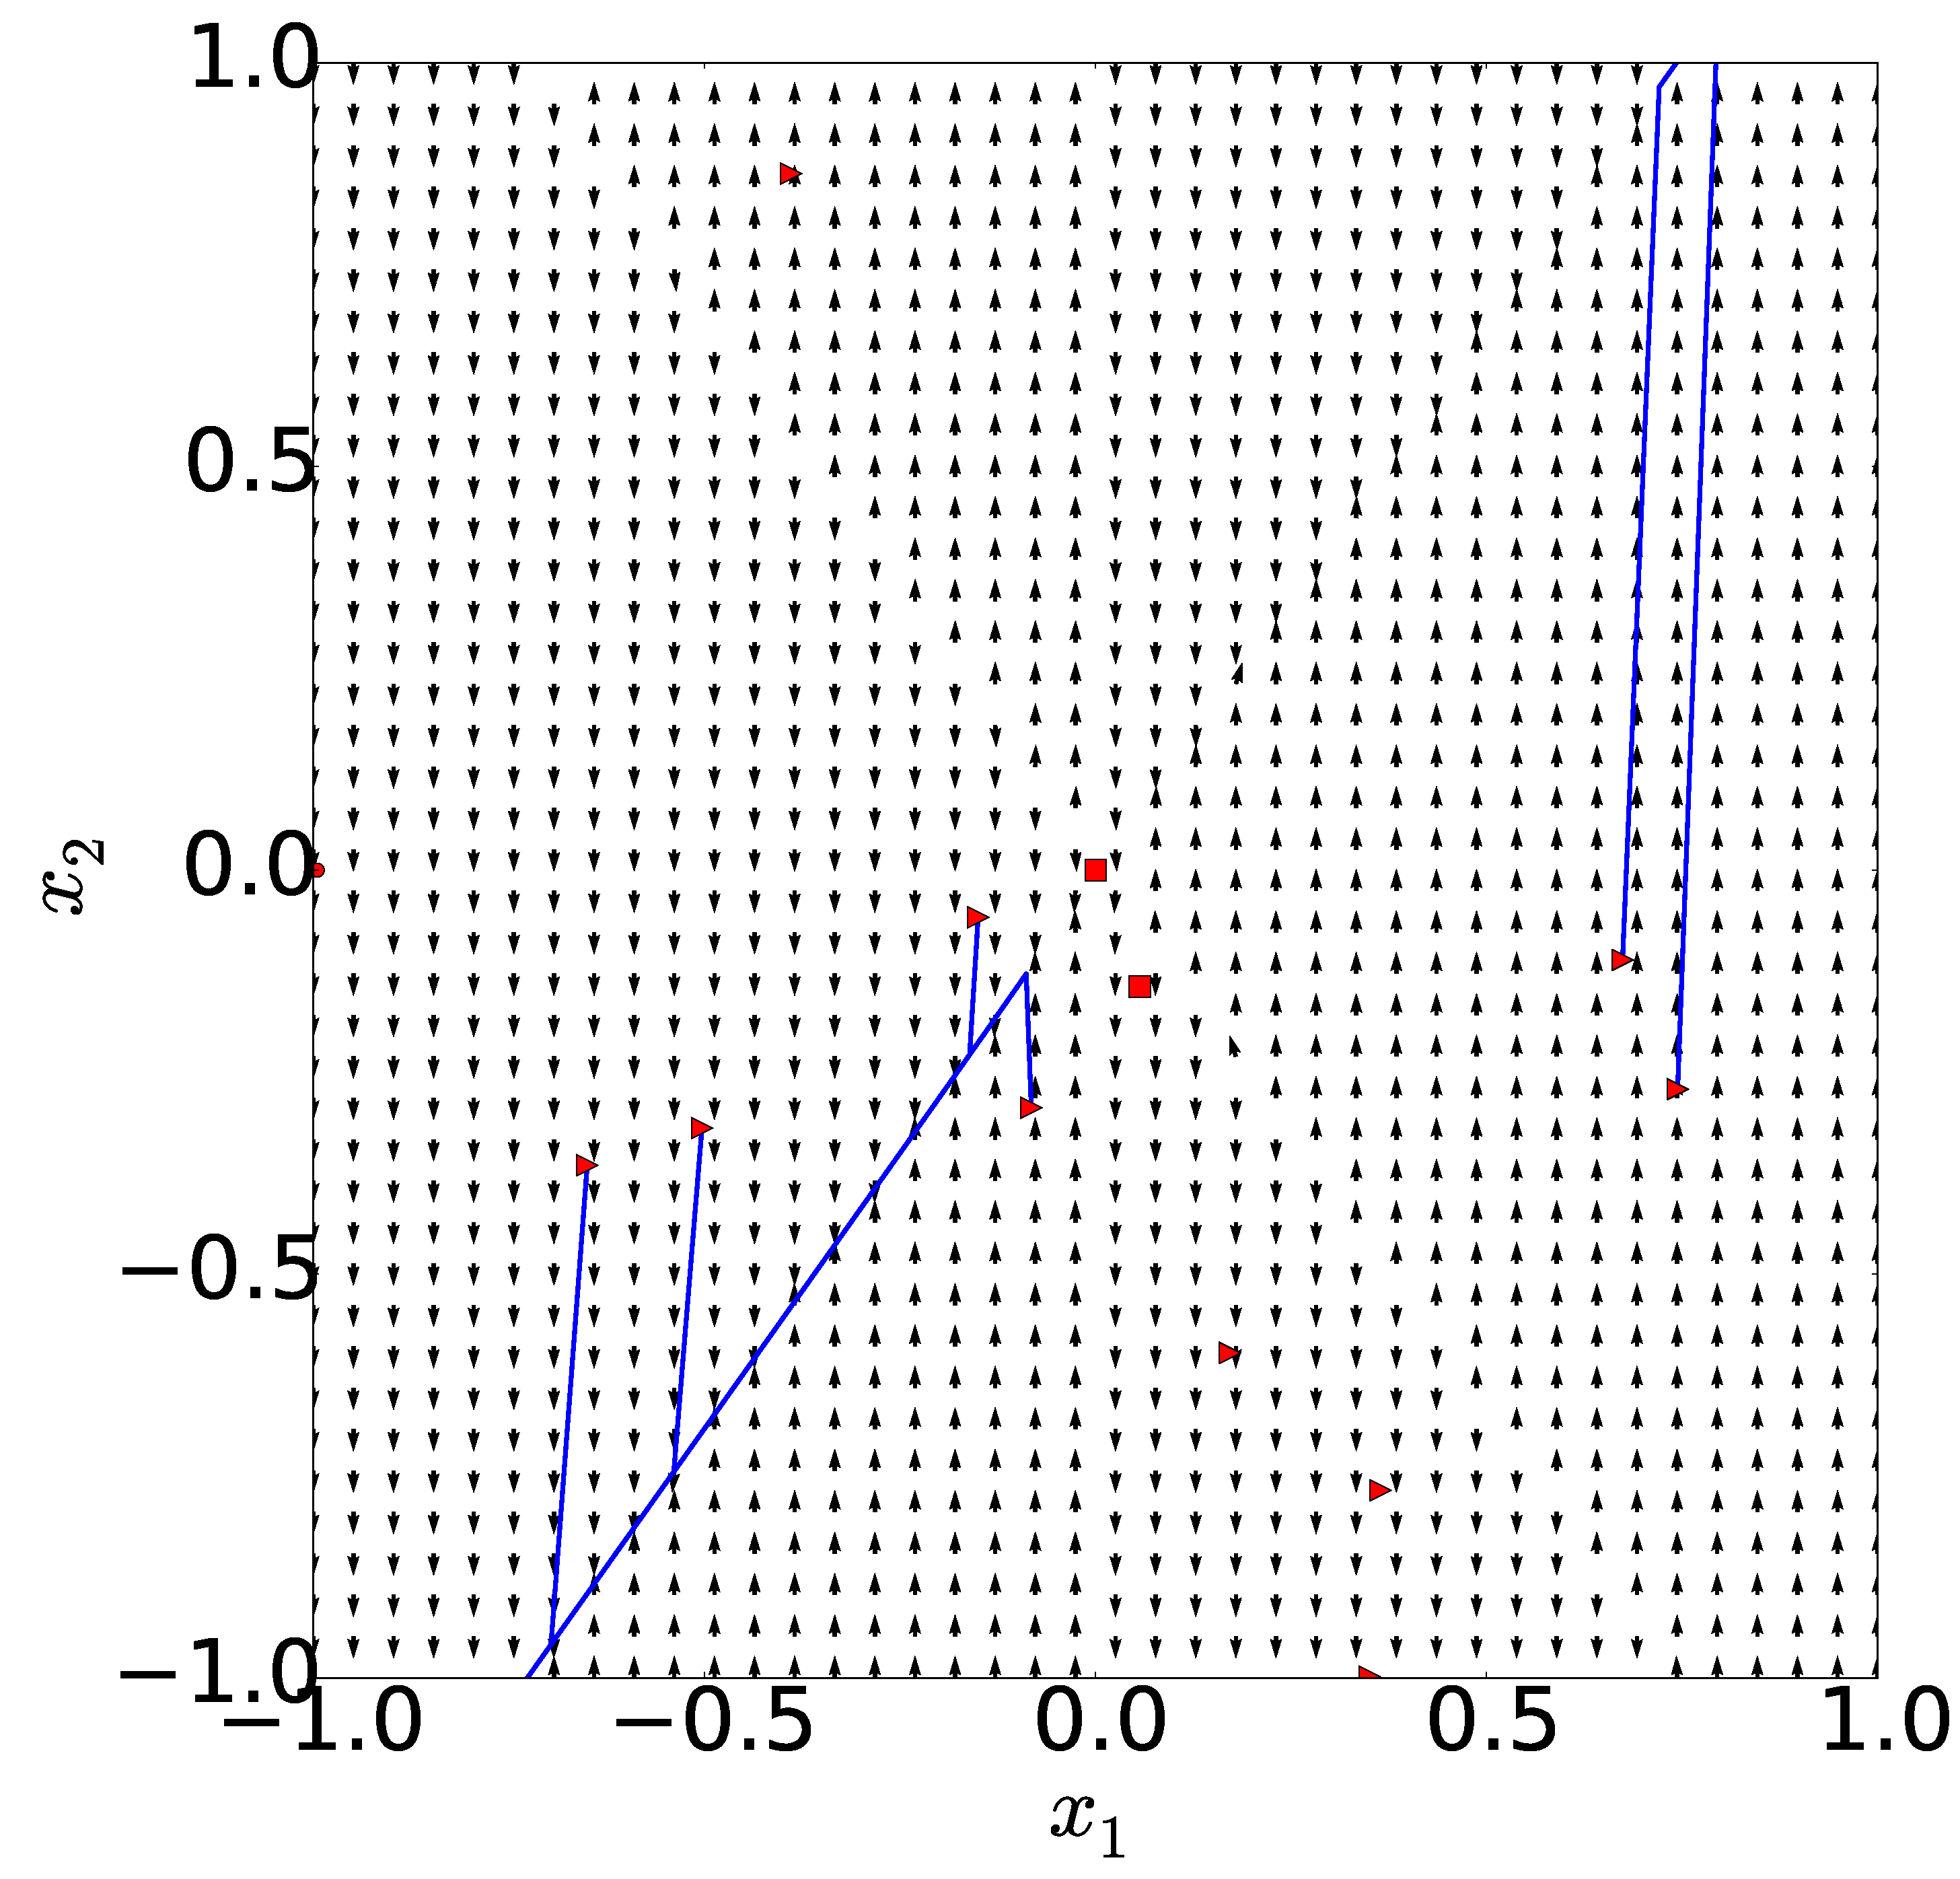
\includegraphics[width=8.0 cm]{figure/phase_portrait_around_x10_-99_x20_-99_1.eps}
		\caption{Case 1 - Expanded function}
	\end{subfigure}
	\begin{subfigure}[h]{8.0 cm}
        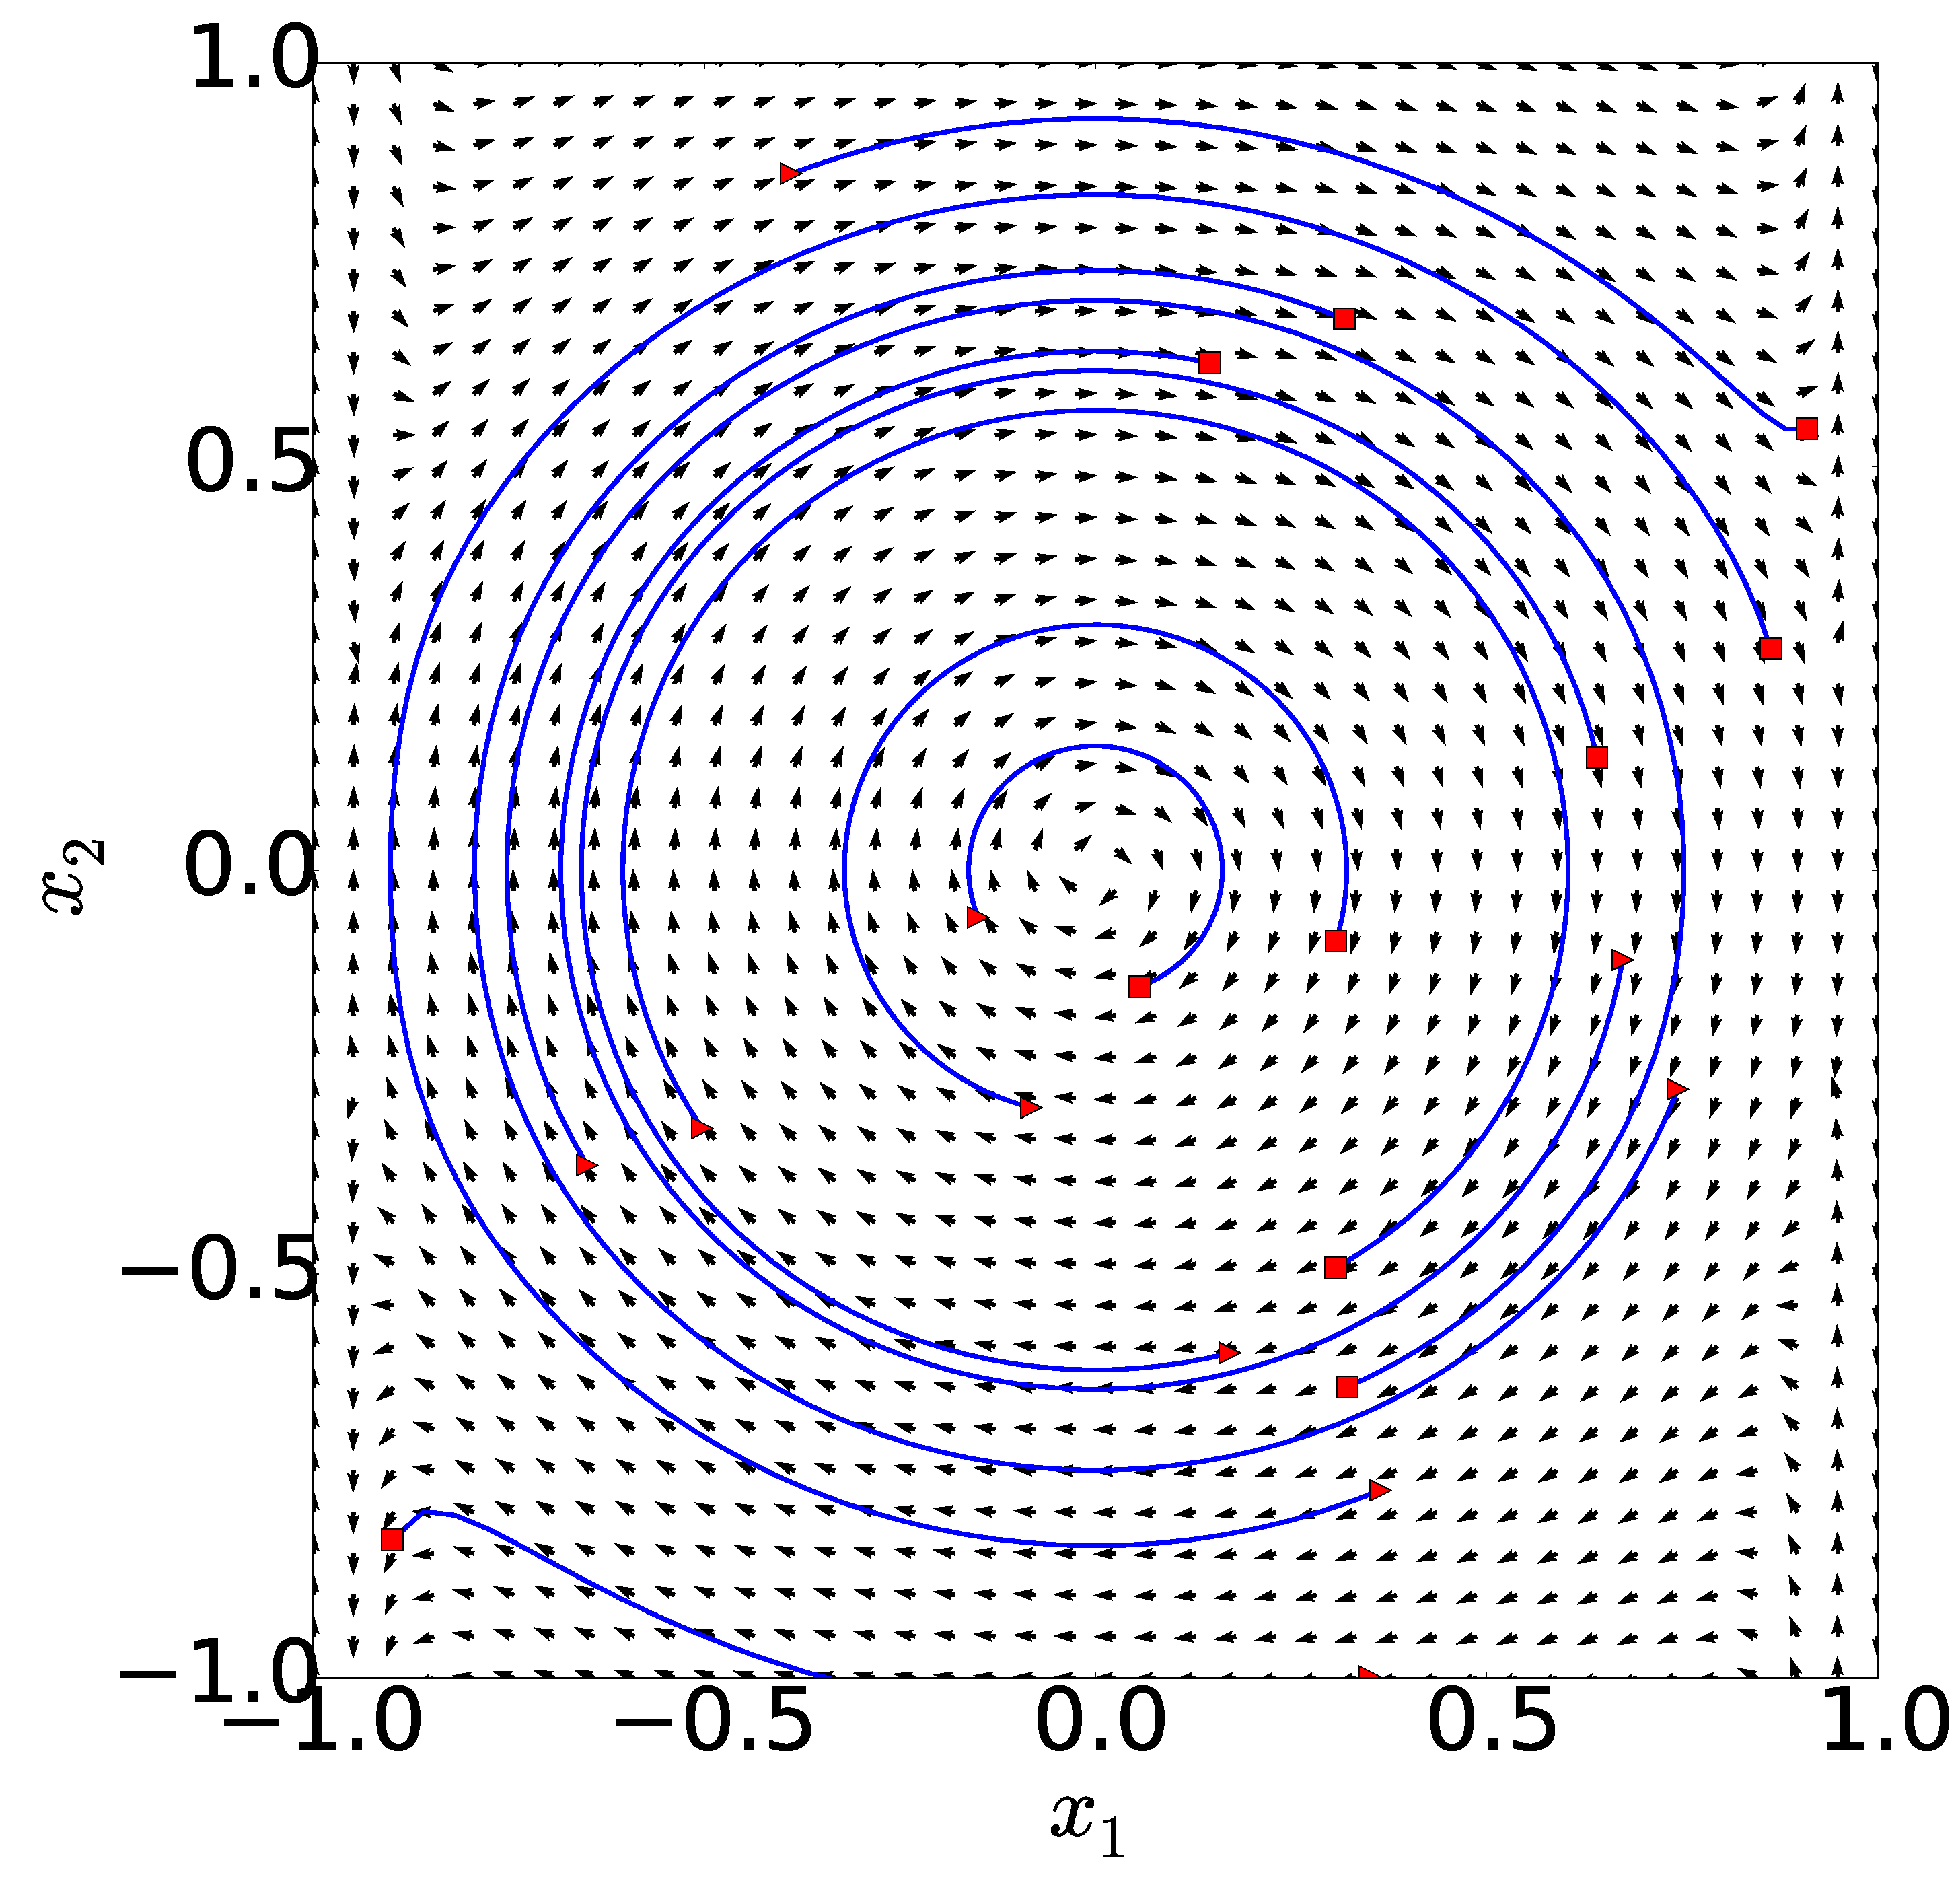
\includegraphics[width=8.0 cm]{figure/1phase_portrait_l2nlcomp1_1.eps}
		\caption{Case 1 - Actual function}
    \end{subfigure}
    \\
    \begin{subfigure}[h]{8.0 cm}
		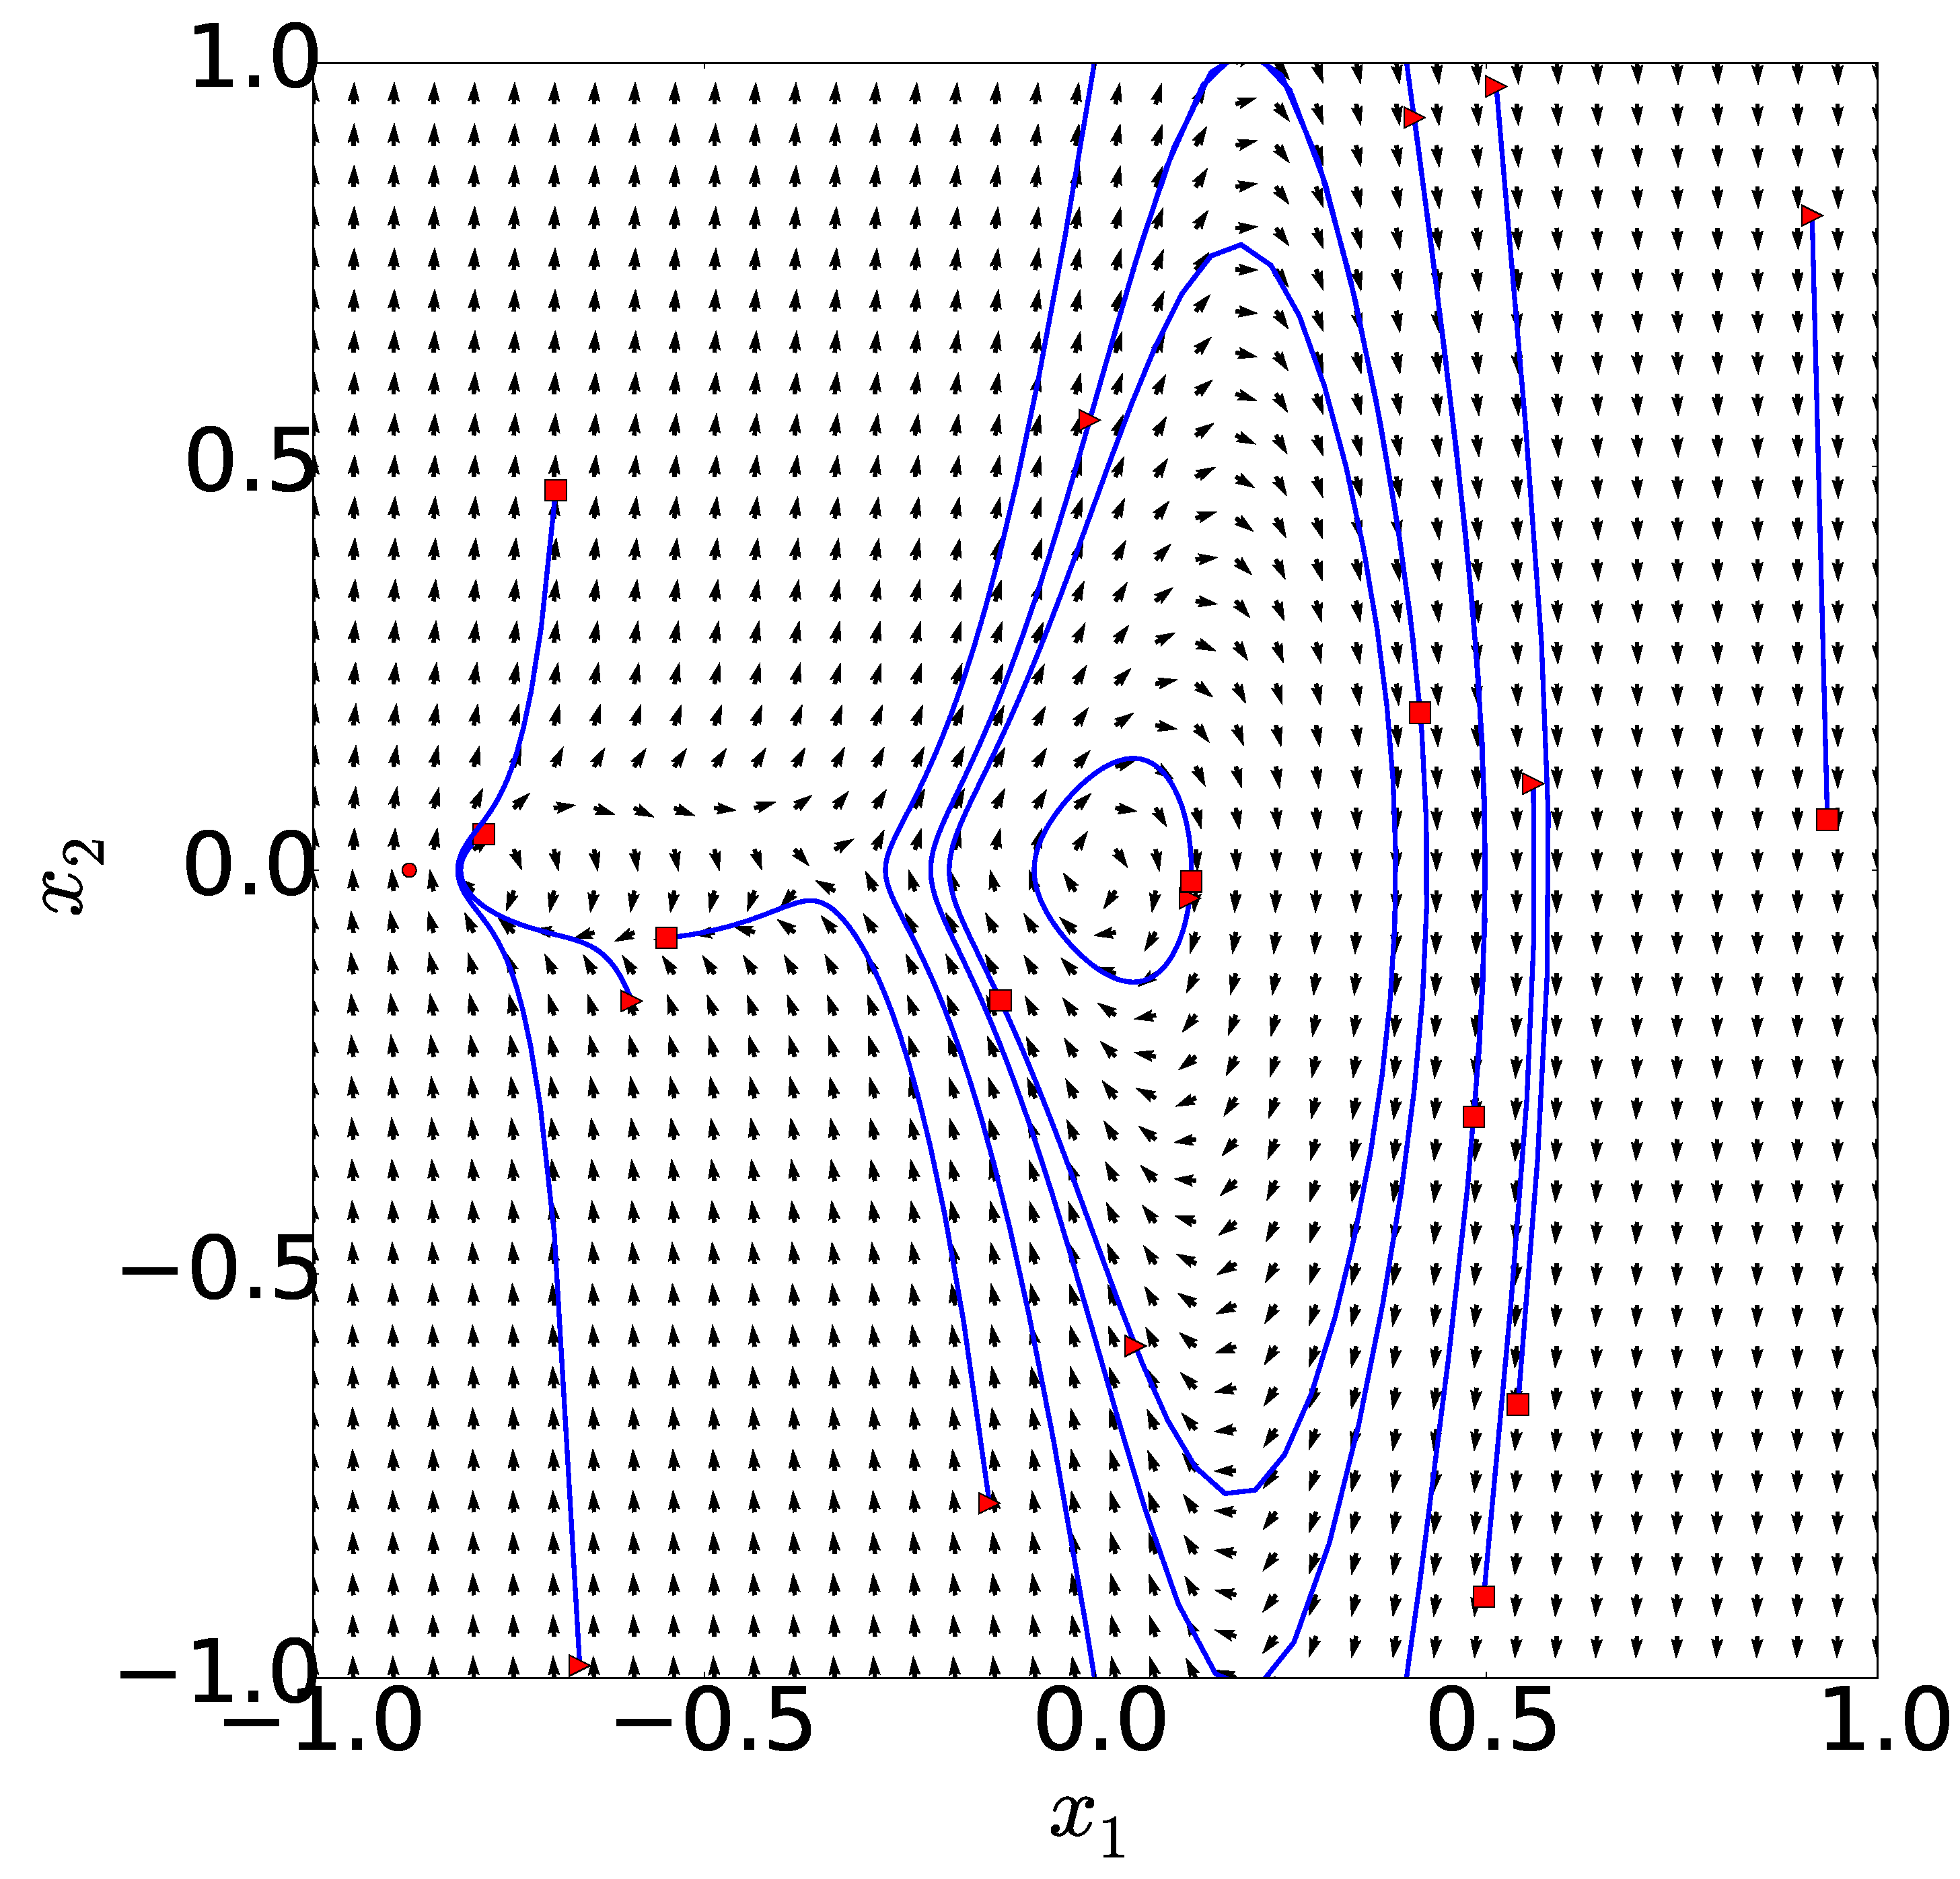
\includegraphics[width=8.0 cm]{figure/phase_portrait_around_x10_-87_x20_-87_2.eps}
		\caption{Case 2 - Expanded function}
	\end{subfigure}
	\begin{subfigure}[h]{8.0 cm}
        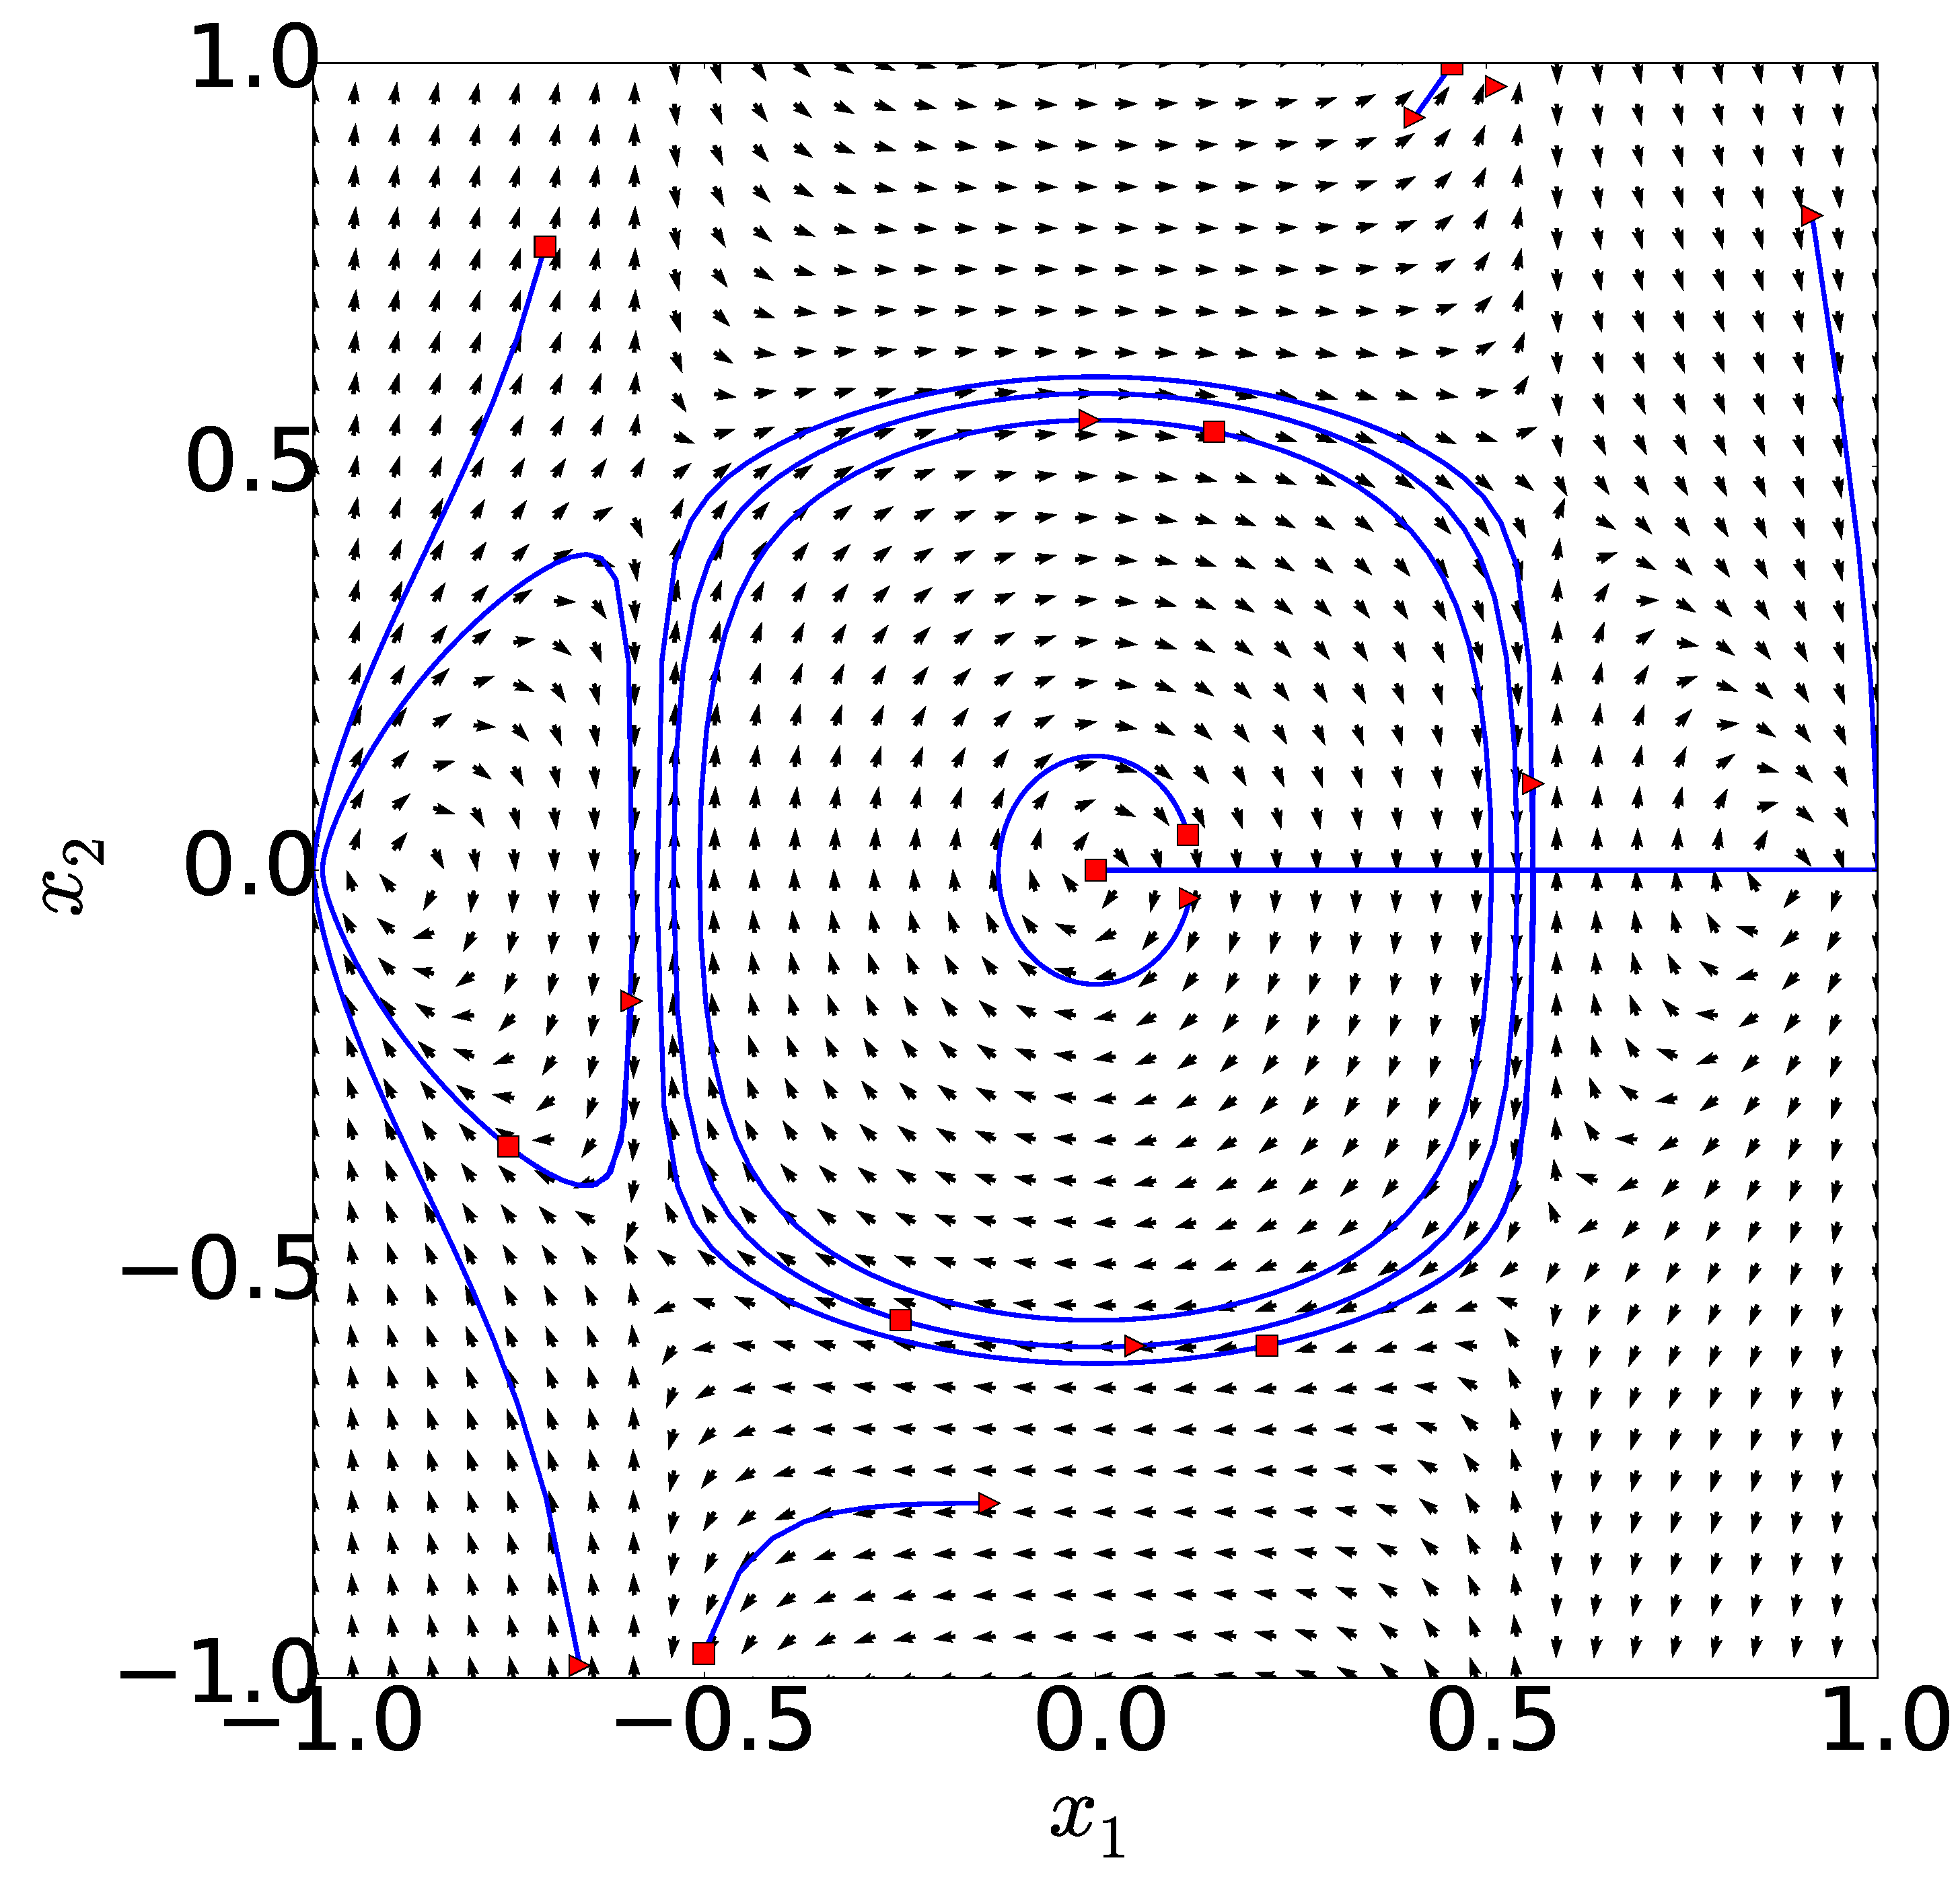
\includegraphics[width=8.0 cm]{figure/1phase_portrait_l2nlcomp1_2.eps}
		\caption{Case 2 - Actual function}
    \end{subfigure}
    \\
    	\begin{subfigure}[h]{8.0 cm}
        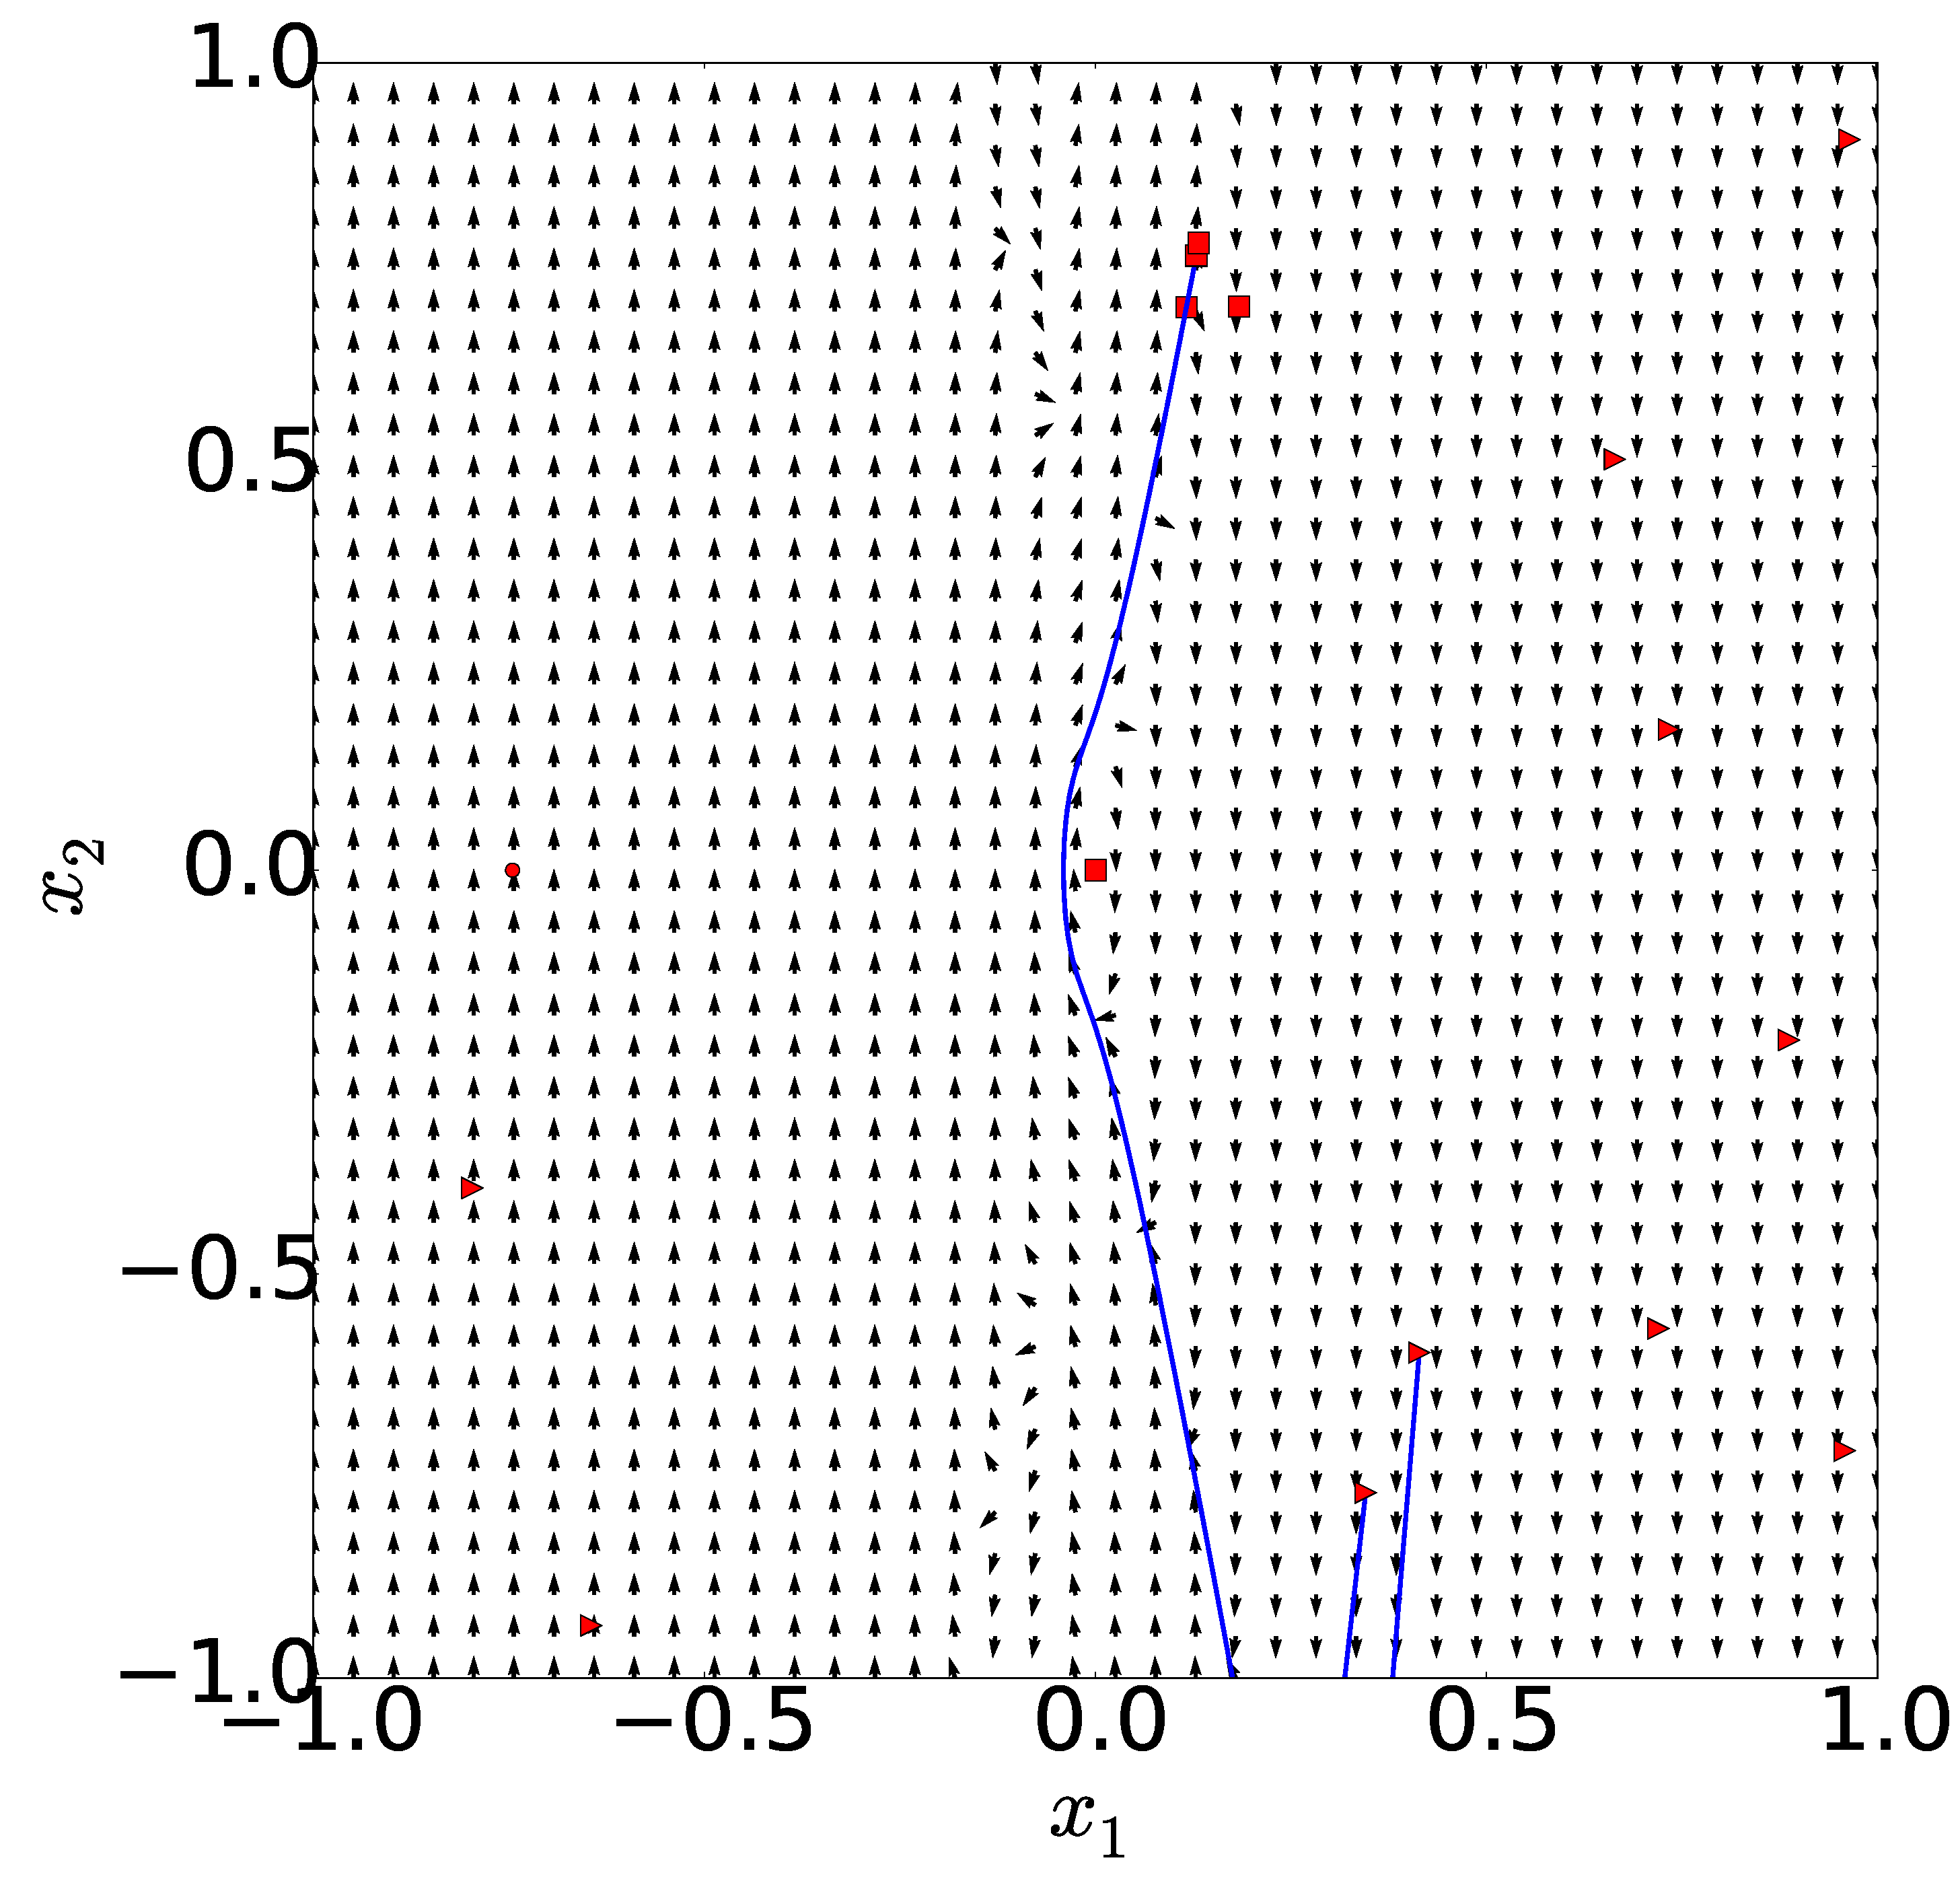
\includegraphics[width=8.0 cm]{figure/phase_portrait_around_x10_-74_x20_-74_3.eps}
		\caption{Case 3 - Expanded function}
    \end{subfigure}
    	\begin{subfigure}[h]{8.0 cm}
        \includegraphics[width=8.0 cm]{figure/1phase_portrait_l2nlcomp1_3.eps}
		\caption{Case 3 - Actual function}
    \end{subfigure}
    \caption{Phase plot for expanded state function around $(-\sqrt{1 - \left( \dfrac{m_1 \epsilon g}{kl} \right)^2}, 0)$. Trajectories start from $\rhd$ and end at $\Box$. All trajectories are integrated for $10$ seconds.}
    \label{fig:PhasePlotExpanded2}
\end{figure}

% ===============================================================
\newpage
\textbf{Problem definition}:
Redo the problems from the in-cla portion, but this time using computer simulations to validate your solutions.

\noindent\hrulefill

% -------------------------------------------------------------------
\textbf{1)} $\ddot{x} - x + x^3 = 0$

The stationary points are calculated by setting $\ddot{x}$ and $\dot{x}$ equal to zero. This will give us the following points:

\begin{equation}
\begin{gathered}
	\mathcal{X} = 0 \\
	\mathcal{X} = \pm 1
\end{gathered}
\end{equation}

This equation can be linearized around each of the stationary points as follows

\begin{equation}
\begin{bmatrix}
	\dot{x}_1 \\
	\dot{x}_2
\end{bmatrix} = 
\begin{bmatrix}
	0 & 1 \\
	1-3\mathcal{X}^2 & 0
\end{bmatrix}
\begin{bmatrix}
	x_1 \\
	x_2
\end{bmatrix}
\end{equation}

Depending on the value of $\mathcal{X}$ we can look at the eigenvalues and eigenvectors of above equation. The eigenvalues with negative real part are the stable stationary point and the eigenvector corresponding with them are the stable manifolds. The eigenvalues with positive real part are the unstable stationary point and the eigenvector corresponding with them are the unstable manifolds. 

For $\mathcal{X} = 0$, we get two eigenvalues, $\lambda_1 = 1.0$ and $\lambda_2 = -1.0$, and two eigenvectors, $\mathbf{v}_1 = [\sqrt{2}, -\sqrt{2}]$ and $\mathbf{v}_2 = [\sqrt{2}, \sqrt{2}]$. The first eigenvector is the unstable manifold and the second one is the stable manifold.

For $\mathcal{X} = \pm 1$, we get two eigenvalues, $\lambda_1 = 1.41i$ and $\lambda_2 = -1.41i$, and two eigenvectors, $\mathbf{v}_1 = [-0.577i, 0.816]$ and $\mathbf{v}_2 = [0.577i, 0.816]$. These are center points since the eigenvalues do not have a real part.

We can plot the phase plot using \texttt{python}. The trajectories are calculated using \texttt{scipy.odeint}. We chose three initial conditions $(-1.5, 0)$, $(1.5, -1)$, $(2, 1.5)$ and integrated for 10 seconds. The result is shown in the following figure.

\begin{figure}[h]
	\centering
	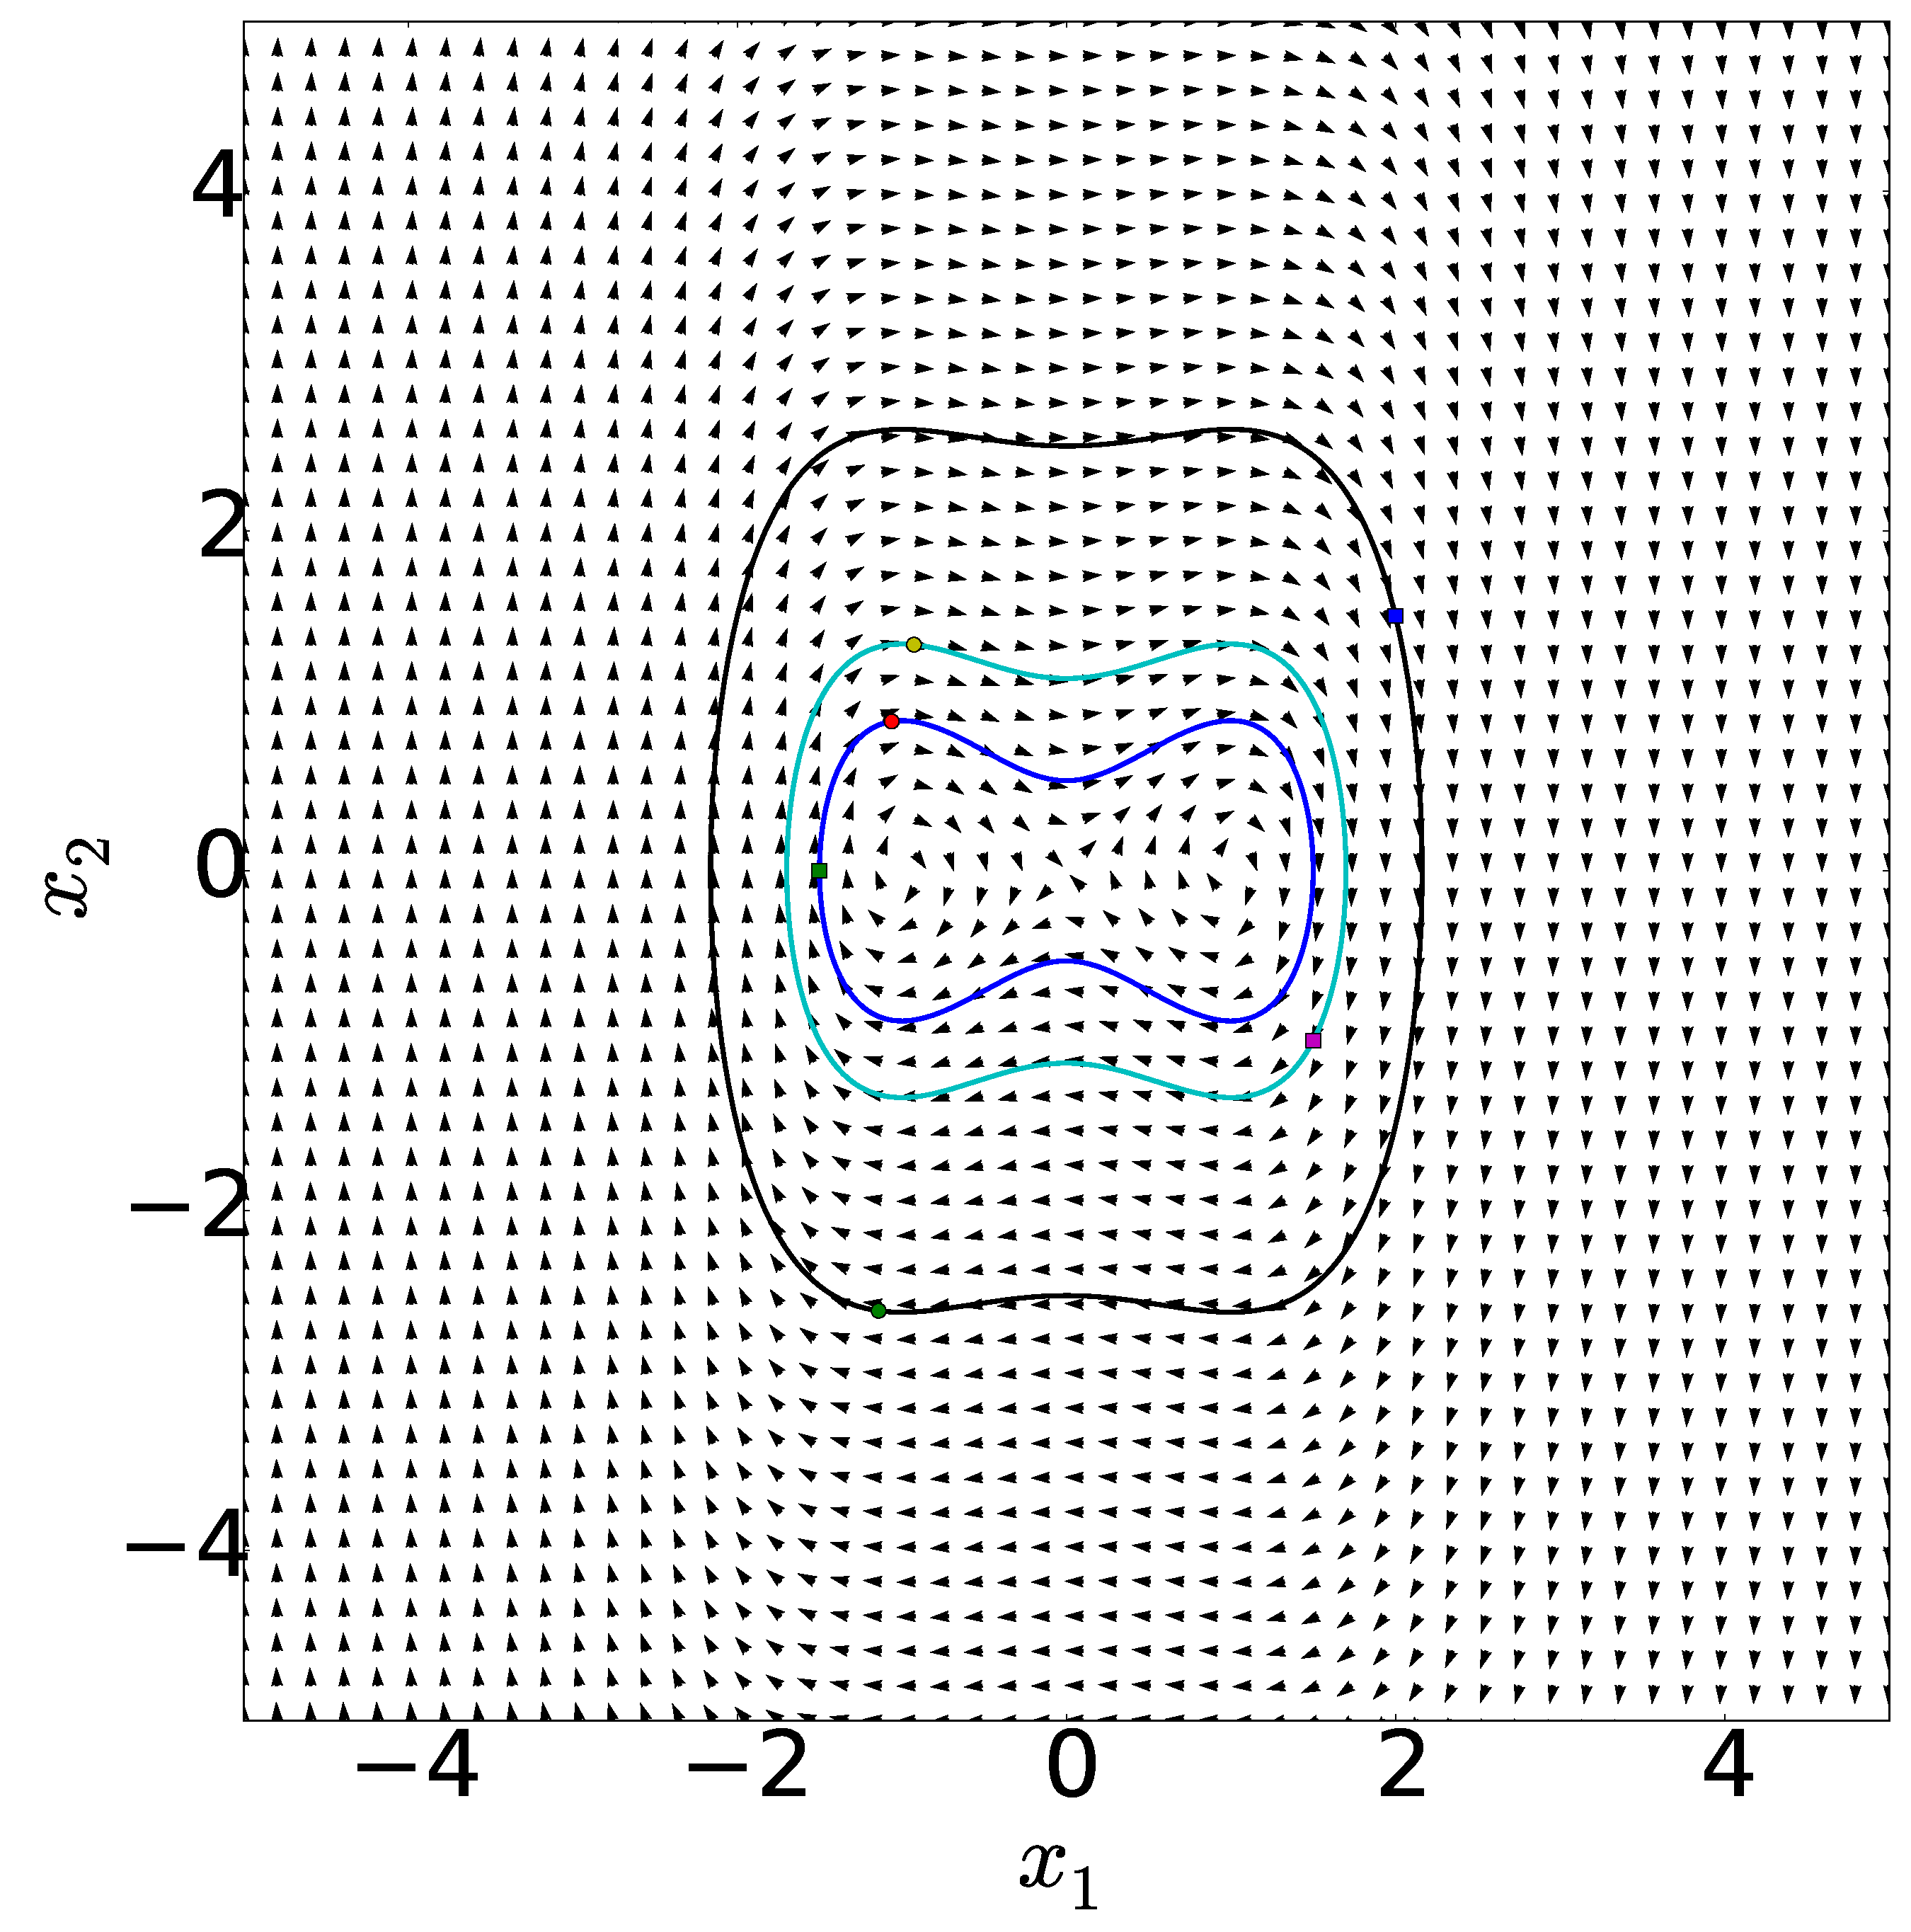
\includegraphics[width=8.0 cm]{figure/1.eps}
	\caption{Phase plot.}
\end{figure}

To check if the system is conservative we use the following equation

\begin{equation}\label{eq:divergence3}
	\frac{\partial \dot{x}}{\partial x} +
	\frac{\partial \dot{y}}{\partial y} +
	\frac{\partial \dot{z}}{\partial z} = 
	0
\end{equation}

Therefore, the system is conservative.
\newpage
% -------------------------------------------------------------------
\textbf{2)} $\ddot{x} + \sin(x) = 0$

The stationary points are calculated by setting $\ddot{x}$ and $\dot{x}$ equal to zero. This will give us the following points:

\begin{equation}
\begin{gathered}
	\mathcal{X} = \pm k \pi \quad , \quad k =0, 1, 2, \dots
\end{gathered}
\end{equation}

Therefore we have infinite number of stationary points. This equation can be linearized around each of the stationary points as follows

\begin{equation}
\begin{bmatrix}
	\dot{x}_1 \\
	\dot{x}_2
\end{bmatrix} = 
\begin{bmatrix}
	0 & 1 \\
	-\cos(\mathcal{X}) & 0
\end{bmatrix}
\begin{bmatrix}
	x_1 \\
	x_2
\end{bmatrix}
\end{equation}

Depending on the value of $\mathcal{X}$ we can look at the eigenvalues and eigenvectors of above equation. The eigenvalues with negative real part are the stable stationary point and the eigenvector corresponding with them are the stable manifolds. The eigenvalues with positive real part are the unstable stationary point and the eigenvector corresponding with them are the unstable manifolds. 

For $\mathcal{X} = 0$, we get two eigenvalues, $\lambda_1 = i$ and $\lambda_2 = -i$, and two eigenvectors, $\mathbf{v}_1 = [0.707, 0707i]$ and $\mathbf{v}_2 = [0.707, -0.707i]$. This is a center point of the solution since the eigenvalues do not have a real part.

For $\mathcal{X} = \pm \pi$, we get two eigenvalues, $\lambda_1 = 1$ and $\lambda_2 = -1$, and two eigenvectors, $\mathbf{v}_1 = [\sqrt{2}, -\sqrt{2}]$ and $\mathbf{v}_2 = [\sqrt{2}, \sqrt{2}]$. The first eigenvector is the unstable manifold and the second one is the stable manifold. This is due to the sign of the eigenvalues.

We can plot the phase plot using \texttt{python}. The trajectories are calculated using \texttt{scipy.odeint}. We chose three initial conditions $(-1.5, 0)$, $(1.5, -1)$, $(2, 1.5)$, $(-3, -2)$ and integrated for 10 seconds. The result is shown in the following figure.

\begin{figure}[h]
	\centering
	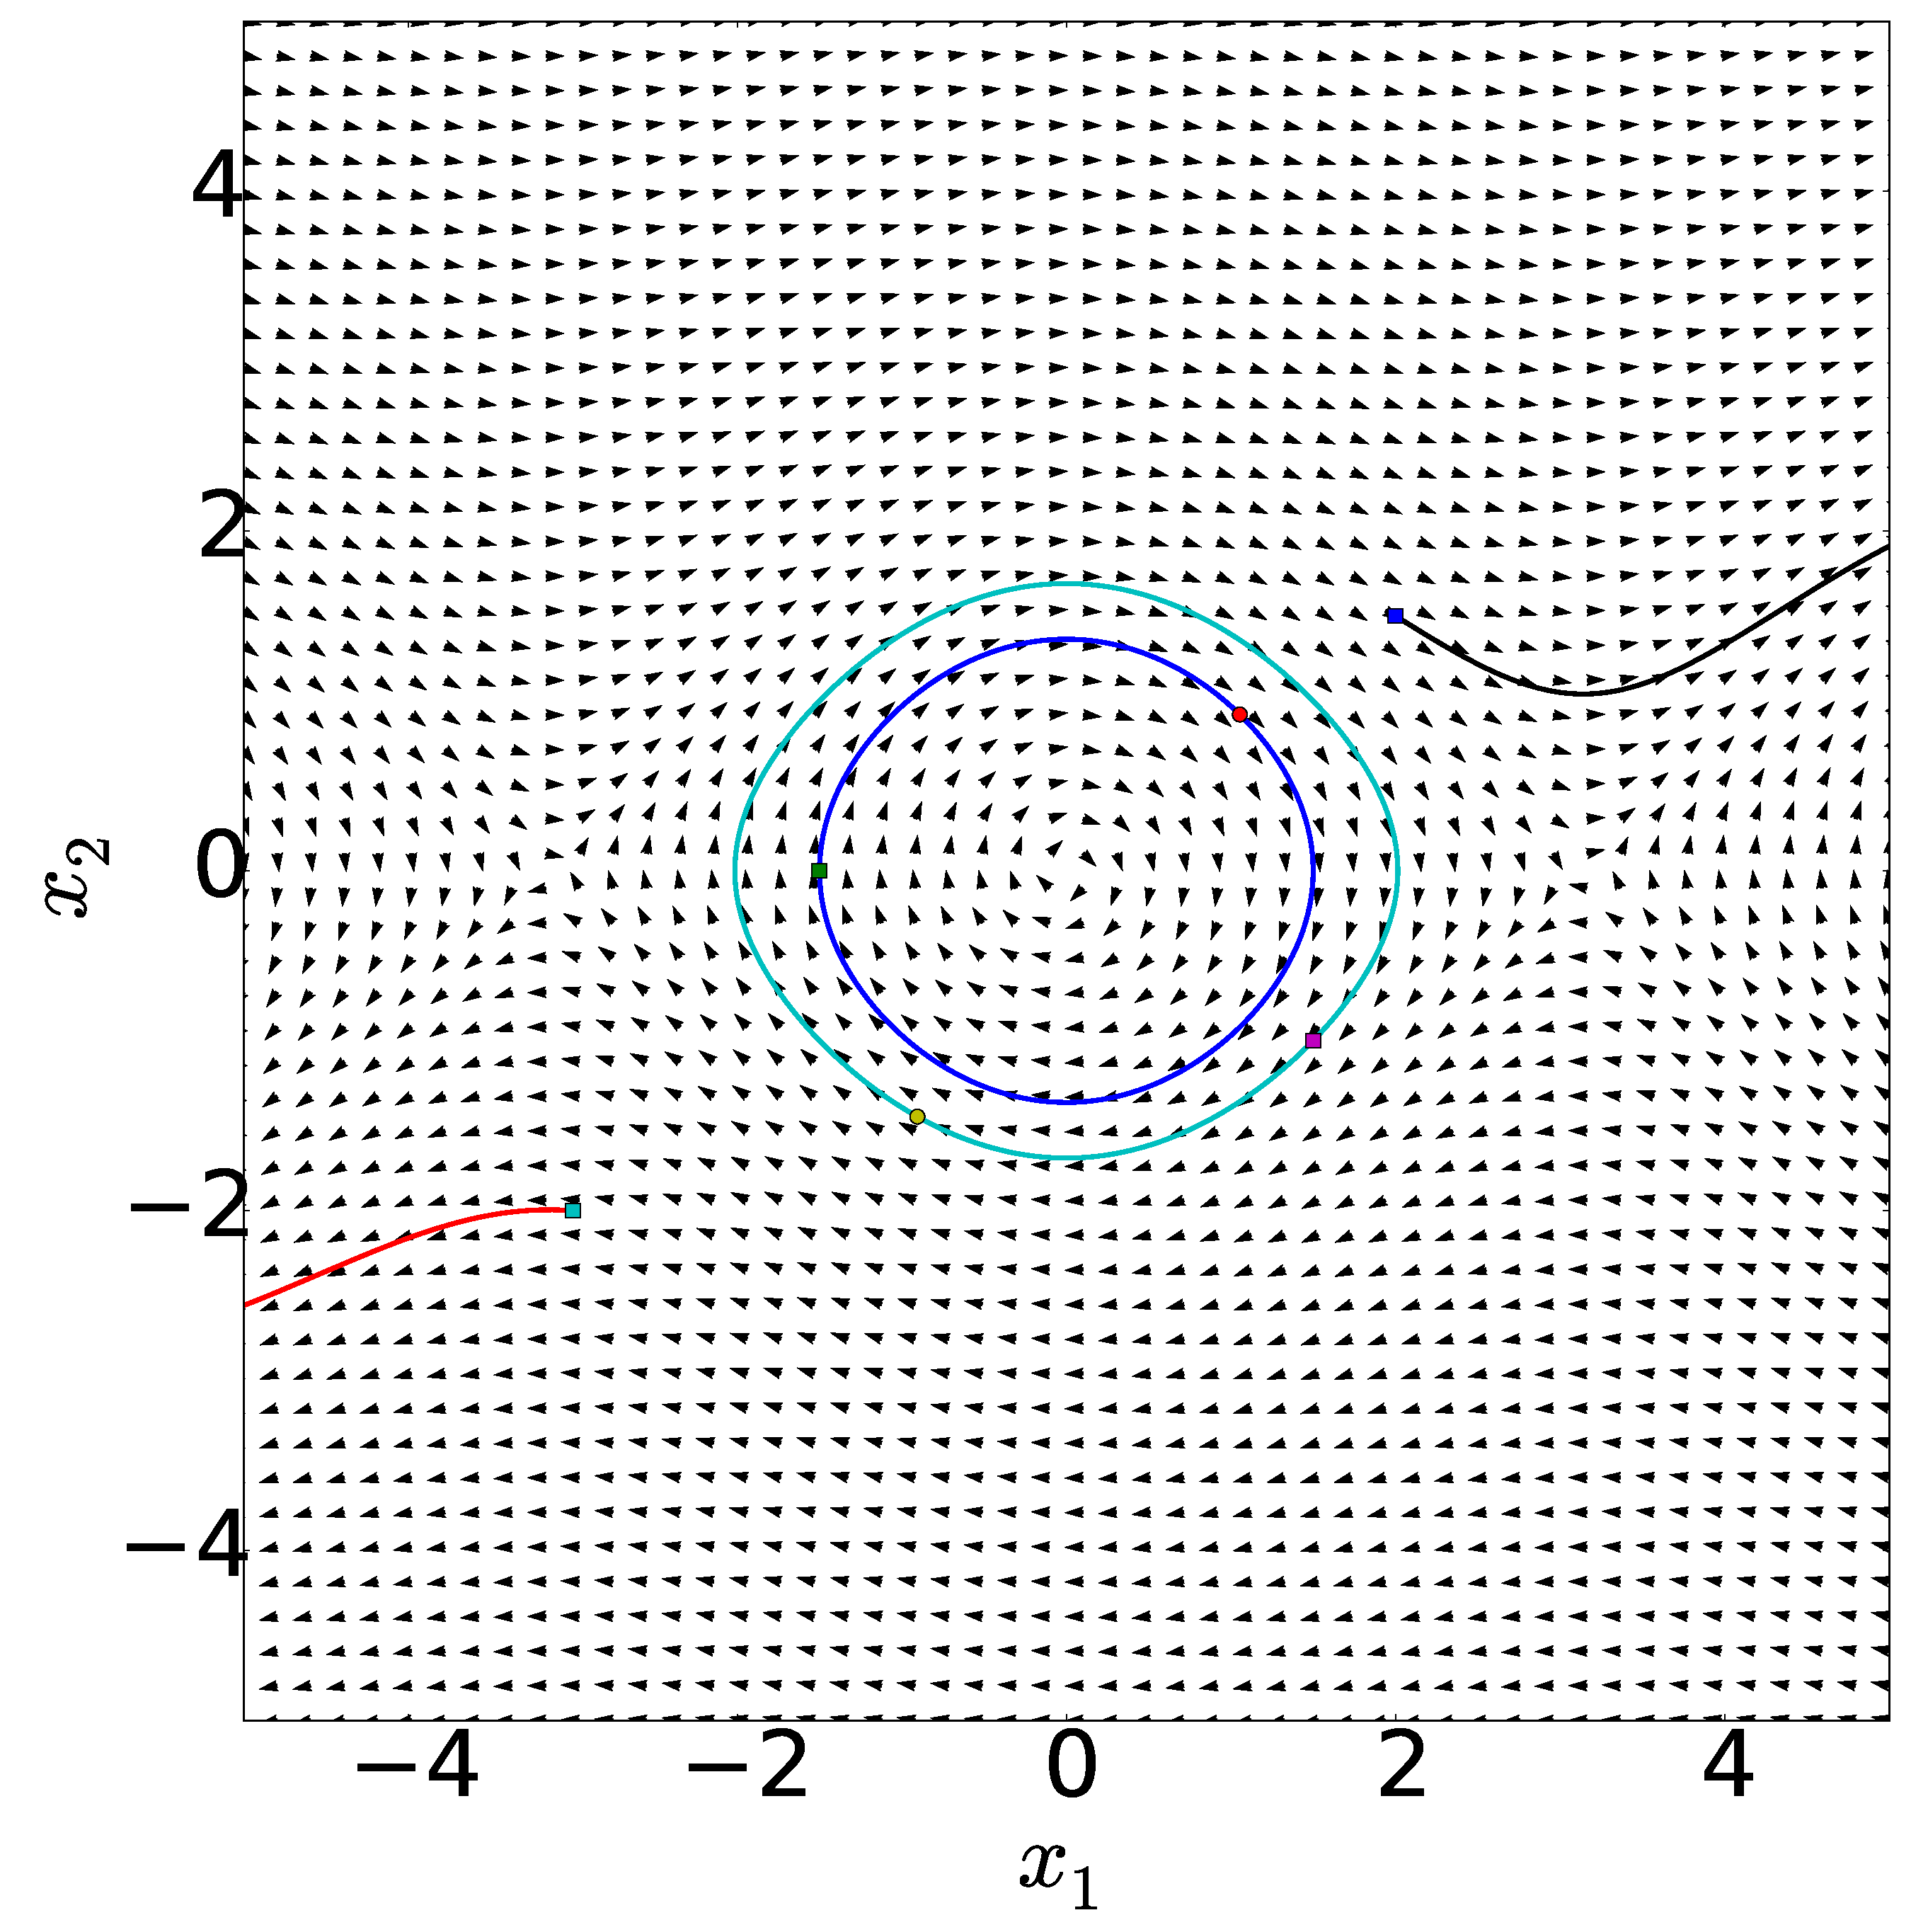
\includegraphics[width=8.0 cm]{figure/2.eps}
	\caption{Phase plot.}
\end{figure}

To check if the system is conservative we use the following equation

\begin{equation}\label{eq:divergence3}
	\frac{\partial \dot{x}}{\partial x} +
	\frac{\partial \dot{y}}{\partial y} +
	\frac{\partial \dot{z}}{\partial z} = 
	0
\end{equation}

Therefore, the system is conservative.
\newpage
% -------------------------------------------------------------------
\textbf{3)} $\dot{x}_1 = x_1 + 2x_2 \quad , \quad \dot{x}_2 = 3x_1 + 2x_2$

The stationary points are calculated by setting $\dot{x}_1$ and $\dot{x}_2$ equal to zero. This will give us the following points:

\begin{equation}
\begin{gathered}
	\mathcal{X} = 0
\end{gathered}
\end{equation}

Therefore we have infinite number of stationary points. This equation can be linearized around each of the stationary points as follows

\begin{equation}
\begin{bmatrix}
	\dot{x}_1 \\
	\dot{x}_2
\end{bmatrix} = 
\begin{bmatrix}
	1 & 2 \\
	3 & 2
\end{bmatrix}
\begin{bmatrix}
	x_1 \\
	x_2
\end{bmatrix}
\end{equation}

To check the characteristic of the stationary point, we can look at the eigenvalues and eigenvectors of above equation. The eigenvalues with negative real part are the stable stationary point and the eigenvector corresponding with them are the stable manifolds. The eigenvalues with positive real part are the unstable stationary point and the eigenvector corresponding with them are the unstable manifolds. 

We get two eigenvalues, $\lambda_1 = -1$ and $\lambda_2 = 4$, and two eigenvectors, $\mathbf{v}_1 = [-0.707, -0.554]$ and $\mathbf{v}_2 = [0.707, -0.832]$. The first eigenvector is the stable manifold and the second one is the unstable manifold. This is due to the sign of the eigenvalues.

We can plot the phase plot using \texttt{python}. The trajectories are calculated using \texttt{scipy.odeint}. We chose three initial conditions $(-1.5, 0)$, $(1.5, -1)$, $(2, 1.5)$, $(-3, 2)$ and integrated for 10 seconds. The result is shown in the following figure.

\begin{figure}[h]
	\centering
	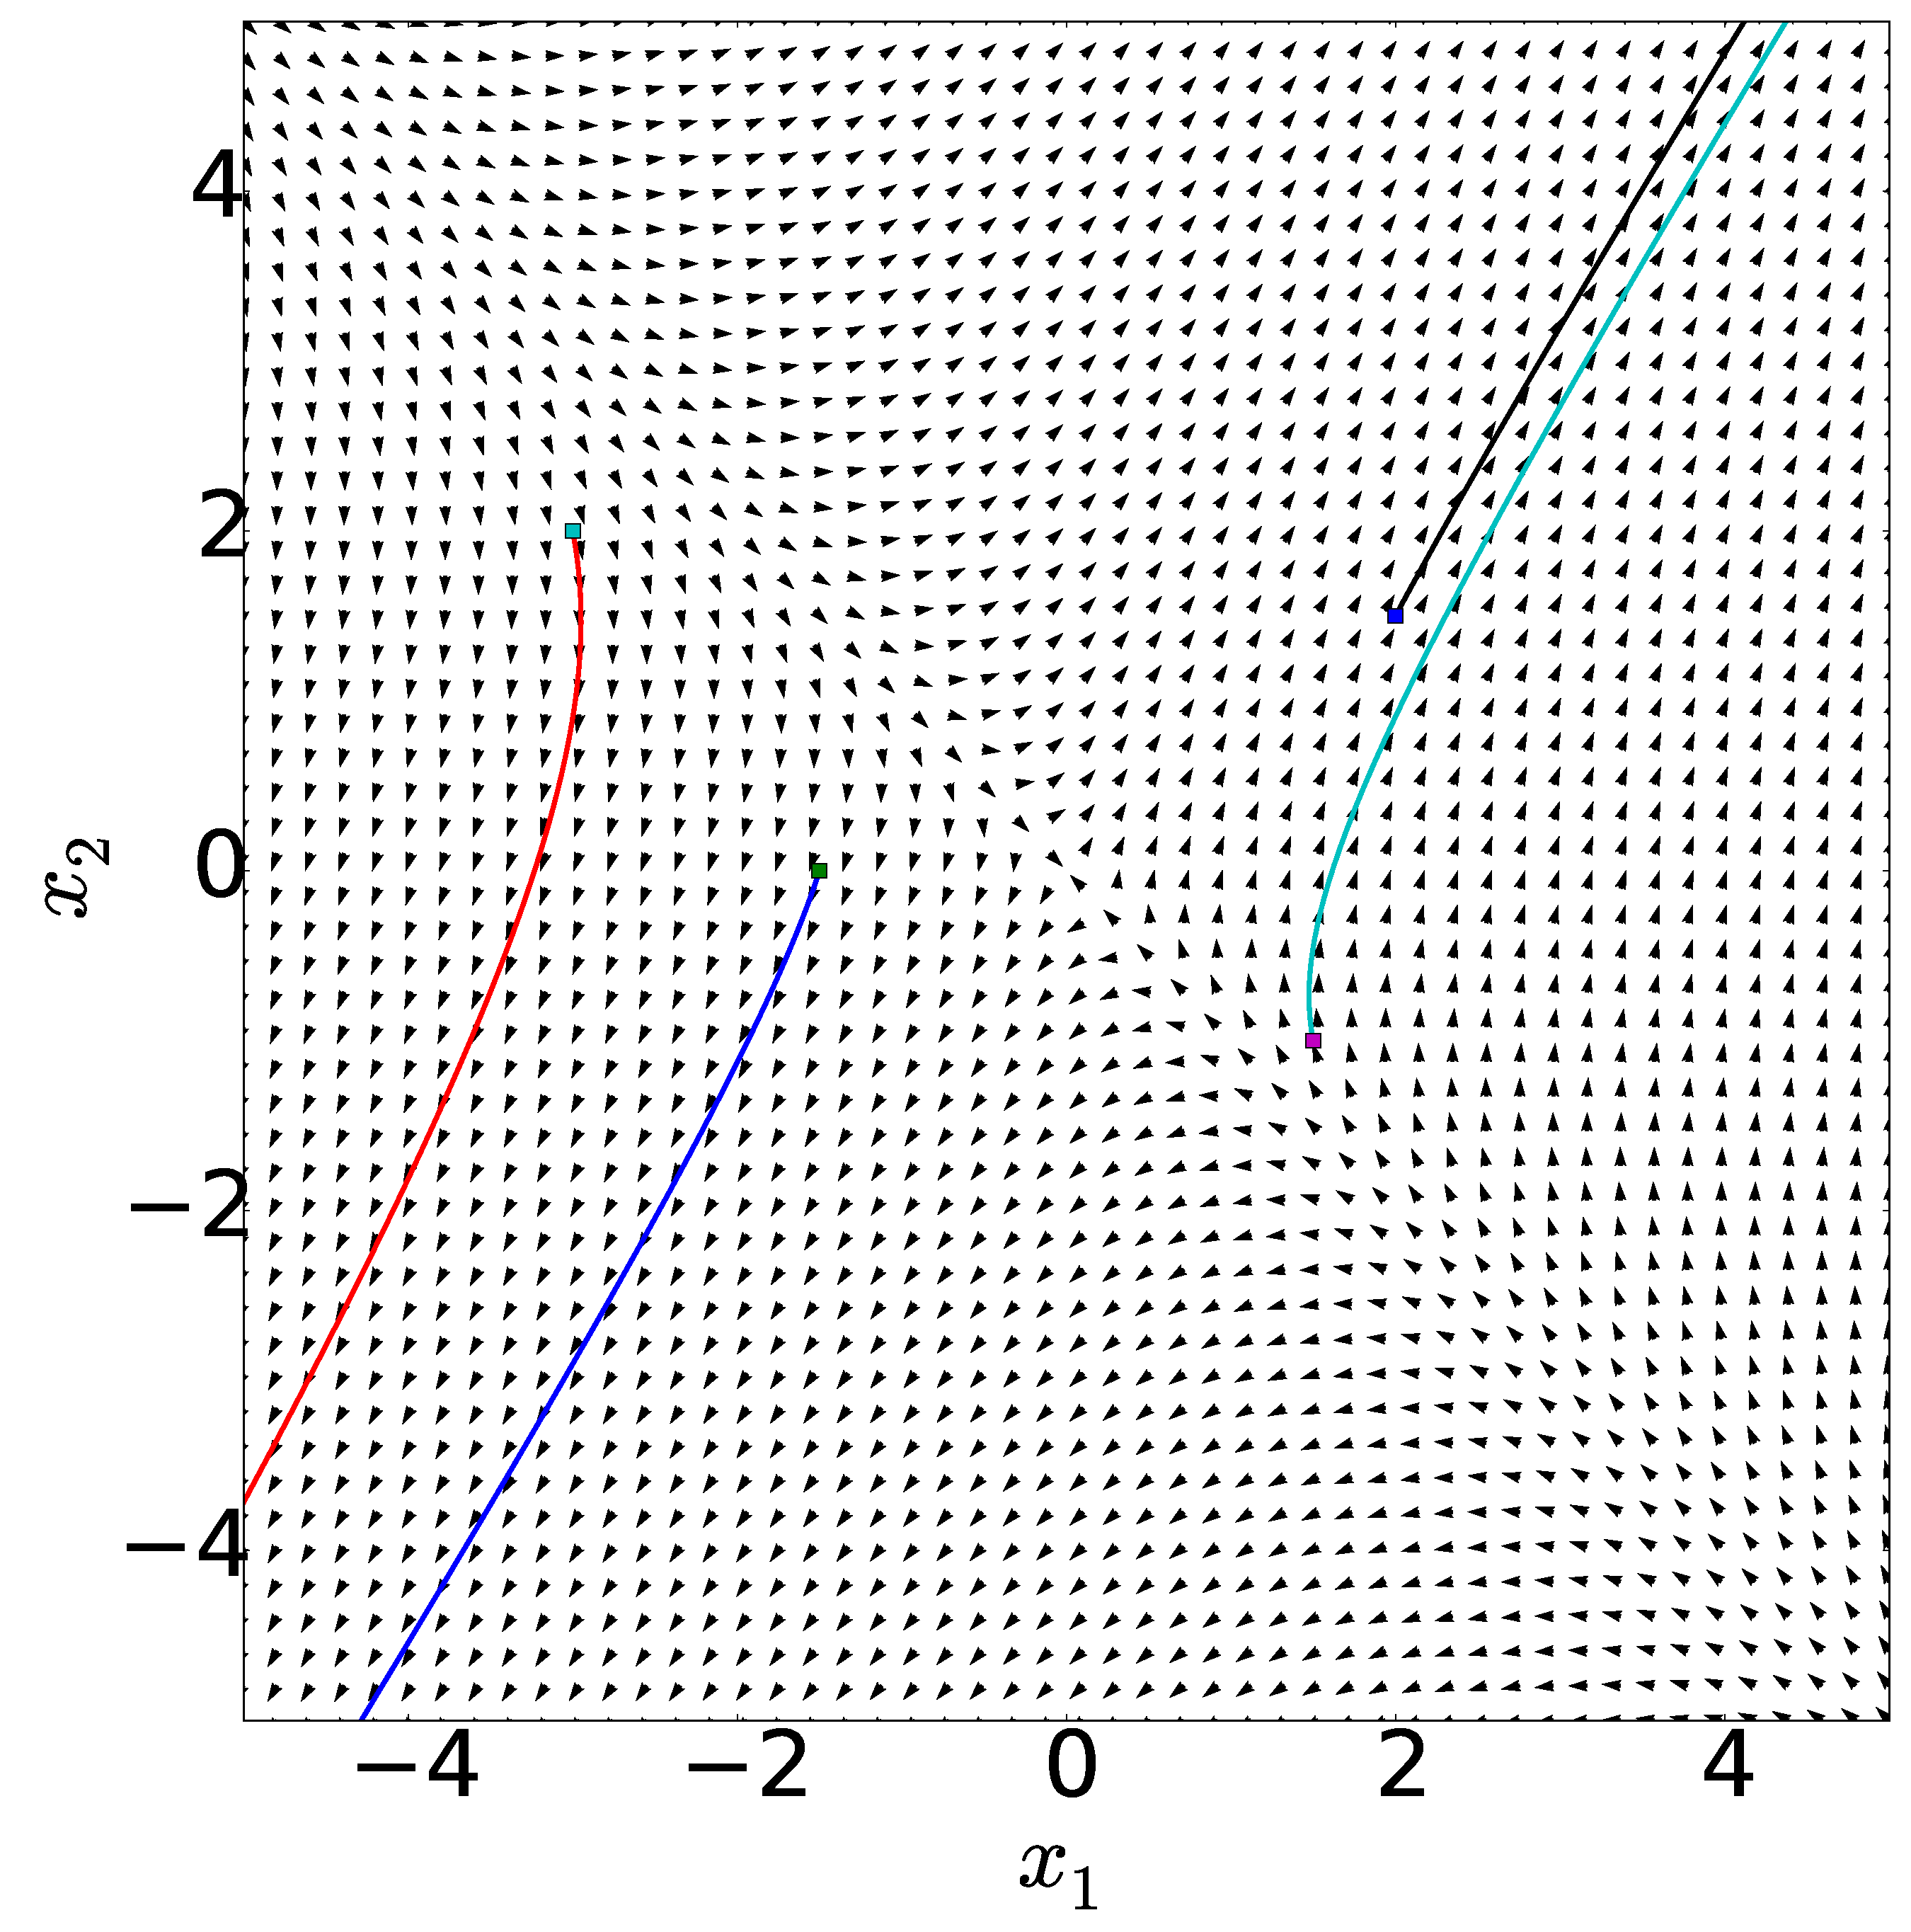
\includegraphics[width=8.0 cm]{figure/3.eps}
	\caption{Phase plot.}
\end{figure}


To check if the system is conservative we use the following equation

\begin{equation}\label{eq:divergence3}
	\left| \det D_{x_{k}} \mathbf{F} \right| = 4 > 1
\end{equation}

Therefore, the system is expanding.
\end{document}